\documentclass[12pt,a4paper,final]{book}
%paquetes por defecto
\usepackage{adjustbox}
\usepackage{amsmath}
\usepackage{amsfonts}
\usepackage{amssymb}
\usepackage{array}
\usepackage[spanish,es-tabla]{babel}

\usepackage{newunicodechar}
\newunicodechar{^^a0}{~}

\usepackage[T1]{fontenc}
\usepackage{graphicx}
%Ruta relativa en el formato de Windows:
\graphicspath{{images/}}
%Paquete para hipervinculos 

\usepackage{glossaries}

%%\usepackage[utf8]{inputenc}

%otros paquetes
\usepackage{booktabs}
%\usepackage{breakurl}
\usepackage{xurl}
\usepackage[font=small, labelfont=bf]{caption}
\usepackage{cite} % para contraer referencias
\usepackage{color}
\usepackage{fancyhdr}
\usepackage{float}
\usepackage[T1]{fontenc}
%\usepackage{fourier}
\usepackage[myheadings]{fullpage}
\usepackage{lastpage}
\usepackage{listings}
\usepackage{listingsutf8}
\usepackage{lmodern}
\usepackage{longtable}
\usepackage[protrusion=true, expansion=true]{microtype}
\usepackage{parskip} % Agrega este paquete para evitar la indentación después de tablas, imágenes, listas, etc.
\usepackage{pstricks,pst-node}
%\usepackage{pxfonts}
\usepackage{rotating}
\usepackage{setspace}
\usepackage{sectsty}
\usepackage{subcaption}
%\usepackage{tablefootnote}
\usepackage{tabularx}
\usepackage[most]{tcolorbox}
\usepackage{url, lipsum}
\usepackage{upquote}
\usepackage{xcolor}
%\usepackage[hidelinks]{hyperref}

\setcounter{topnumber}{8}
\setcounter{bottomnumber}{8}
\setcounter{totalnumber}{8}

% Definir los colores
\definecolor{codegreen}{rgb}{0,0.6,0}
\definecolor{codegray}{rgb}{0.5,0.5,0.5}
\definecolor{codepurple}{rgb}{0.58,0,0.82}
\definecolor{backcolour}{rgb}{0.95,0.95,0.92}
\definecolor{azulcielo}{RGB}{135,206,235}
\definecolor{lightblue}{rgb}{0.68, 0.85, 0.90}

%Espaciado de la indentación de los párrafos
\setlength{\parindent}{18pt}

% Estilo de fuente
\lstdefinestyle{mystyle}{
	backgroundcolor=\color{backcolour},
	basicstyle=\ttfamily\footnotesize,
	breakatwhitespace=false,
	breaklines=true,
	captionpos=b,
	commentstyle=\color{codegreen},
	keepspaces=true,
	keywordstyle=\color{magenta},
	numbers=left,
	numbersep=5pt,
	numberstyle=\tiny\color{codegray},
	escapechar=\\
	stringstyle=\color{codepurple},
	showspaces=false,
	showstringspaces=false,
	showtabs=false,
	tabsize=2
}

% Configuración del paquete listings
\lstset{style=mystyle}
\lstset{escapechar=\%}

\lstset{
	language=Java,
	basicstyle=\ttfamily\footnotesize,
	showstringspaces=false,
	keywordstyle=\bfseries\color{blue},
	commentstyle=\itshape\color{gray},
	stringstyle=\color{orange},
	numbers=left,
	numberstyle=\tiny,
	breaklines=true,
	breakatwhitespace=true,
	tabsize=4
}

\newtcolorbox{TextBox}[2]{
	colback=blue!10,
	colframe=azulcielo,
	coltext=black,
	arc=4pt,
	boxrule=1.2pt,
	leftrule=10pt,
	rightrule=0pt,
	toprule=2pt,
	bottomrule=0pt,
	enhanced,
	%fontupper=\sffamily\small,
	title=#1,
	coltitle=black,
	sharpish corners,
	drop shadow,
	sharp corners,
	#2
}

%%\DeclareUnicodeCharacter{00A0}{~}
%\setlength{\parindent}{0cm} esto sirve para quitar todas las sandrias de los parragos
\setlength{\parskip}{2.5mm} % separacion entre parrafos
\renewcommand{\lstlistingname}{Listado} %espaniol del listing

\newglossary[glg]{general}{gls}{glo}{Glosario}
\makeglossaries

%Tamaño de texto fijo para que el tamaño del papel no influya.
%\setlength{\textheight}{650pt}
%\setlength{\textwidth}{500pt}
\graphicspath{ {./images/} }
%NO por ser el último (casi) que se debe cargar
\usepackage{hyperref}
\hypersetup{
	colorlinks=true,
	linkcolor=black,
	filecolor=magenta,
	urlcolor=blue,
	citecolor=black,
}

\usepackage{footnotehyper}
\usepackage{tablefootnote}

\begin{document}
	%ajustar algunas longitudes para invocar el problema
	\baselineskip15pt
	
	\author{\textbf{\Large {Gleiston Cicerón Guerrero Ulloa}}}
	\title{Aplicaciones Distribuidas: Un enfoque desde la Ingeniería de Software}
	\date{}
	
	\maketitle
	\pagenumbering{Roman} % para comenzar la numeracion de paginas en numeros
	\chapter*{Prefacio}

\noindent
La era digital en la que vivimos ha sido testigo de un avance exponencial en la forma en que las tecnologías de la información transforman nuestras vidas cotidianas. Los sistemas de software, en particular, han evolucionado de aplicaciones independientes y aisladas a sistemas complejos y distribuidos que interactúan entre sí para ofrecer servicios innovadores y mejorar nuestras experiencias digitales. Es en este contexto donde las aplicaciones distribuidas se han convertido en un pilar fundamental para el desarrollo de software moderno.

Este libro se ha concebido como una guía completa para estudiantes de Ingeniería de Software que buscan profundizar su comprensión de las aplicaciones distribuidas. A través de sus páginas, exploraremos los fundamentos de las aplicaciones distribuidas, desde su arquitectura hasta los modelos de comunicación, así como los desafíos únicos que presentan en términos de seguridad, escalabilidad y consistencia de datos. También analizaremos las tecnologías de software que son fundamentales para el desarrollo de estas aplicaciones, incluidos los lenguajes de programación, frameworks, protocolos de comunicación, y herramientas de desarrollo.

Uno de los aspectos más críticos en el desarrollo de aplicaciones distribuidas es la gestión eficiente del almacenamiento de datos. Por esta razón, dedicaremos un capítulo completo a explorar las bases de datos distribuidas, los sistemas de archivos distribuidos, y las técnicas de replicación y particionamiento que son esenciales para garantizar la consistencia y disponibilidad de los datos en entornos distribuidos.

En el corazón de este libro, también encontrará un capítulo dedicado al proceso de desarrollo de aplicaciones distribuidas, desde el diseño y modelado hasta la implementación, pruebas, despliegue y mantenimiento. A través de casos de estudio, ilustraremos cómo las aplicaciones distribuidas están transformando industrias y sectores enteros, desde la computación en la nube hasta los sistemas de procesamiento de datos en tiempo real, y las aplicaciones de Internet de las cosas (IoT).

Concluiremos este libro explorando el futuro de las aplicaciones distribuidas, analizando las tendencias emergentes, los desafíos futuros, y las oportunidades de investigación y desarrollo que se presentan en este campo en constante evolución.

Esperamos que este libro le brinde una base sólida y un amplio conocimiento sobre las aplicaciones distribuidas, y que le inspire a explorar más a fondo este apasionante campo de la Ingeniería de Software.

Bienvenido a la fascinante travesía de las aplicaciones distribuidas.
	\tableofcontents
	\pagenumbering{arabic}
	\chapter*{Introducción}
Las aplicaciones distribuidas representan una respuesta integral a la necesidad emergente de sistemas capaces de gestionar procesos complejos, escalables y geográficamente dispersos en un mundo cada vez más globalizado y digitalizado. La dependencia de sistemas que operan efectiva y eficientemente a través de múltiples ubicaciones y zonas horarias se ha incrementado de manera significativa. En este contexto, se considera una realidad cotidiana la colaboración en tiempo real entre equipos de diferentes partes del mundo, un fenómeno facilitado en gran medida por las aplicaciones distribuidas.

Desde los inicios de las redes de computadoras, ha existido un deseo constante de compartir recursos, información y capacidades. A medida que la tecnología ha avanzado, las ambiciones en torno a la capacidad de procesar, analizar y actuar sobre los datos se han ampliado. Las aplicaciones distribuidas se erigen como el nexo entre estas ambiciones y la realidad tangible, permitiendo la colaboración entre múltiples sistemas y componentes, que operan como una entidad cohesiva, independientemente de las distancias físicas que los separan.

En este libro, se proporcionará una comprensión profunda de que las aplicaciones distribuidas no son simplemente una evolución de las aplicaciones monolíticas tradicionales. Por el contrario, representan una redefinición completa de cómo debe abordarse el diseño, desarrollo y mantenimiento del software en la actualidad. Se ha transitado de la centralización en un único servidor o sistema hacia un escenario en el que múltiples sistemas, a menudo distribuidos globalmente, cooperan armoniosamente.

El primer capítulo se dedicará a explorar la definición, características y relevancia actual de las aplicaciones distribuidas, proporcionando una visión integral que servirá como base para los capítulos subsiguientes. A través de ejemplos cotidianos, se ilustrará la omnipresencia de estas aplicaciones en diversos ámbitos de la vida diaria, desde las redes sociales hasta los sistemas bancarios que procesan transacciones en tiempo real.

Es importante señalar que, a pesar de las numerosas ventajas que ofrecen las aplicaciones distribuidas, también presentan desafíos únicos. La complejidad intrínseca de diseñar sistemas que operan en múltiples ubicaciones, junto con la necesidad de asegurar la confidencialidad y privacidad de los datos, así como gestionar la escalabilidad y el rendimiento, son algunos de los aspectos que se abordarán en detalle en este libro.

Por ende, este libro busca no solo proporcionar una comprensión teórica, sino también práctica, de cómo se conceptualizan, implementan y mantienen las aplicaciones distribuidas. A través de cada página, se aspira a acercar al lector un paso más hacia la conversión en un experto en el campo, capaz de comprender y contribuir al paisaje en constante evolución de la Ingeniería de Software.

Por consiguiente, se invita al lector a emprender este viaje hacia el fascinante universo de las aplicaciones distribuidas. Bienvenido a un mundo donde la colaboración, la innovación y la tecnología convergen para crear soluciones que transforman la realidad tal como la conocemos.
	\chapter{Introducción a las aplicaciones distribuidas}
\noindent
Las aplicaciones distribuidas representan un pilar fundamental en el desarrollo de software moderno, desempeñando un rol crucial en la manera en que los sistemas informáticos interactúan y colaboran en un entorno globalizado y digitalizado. En este capítulo, se abordarán los conceptos clave relacionados con las aplicaciones distribuidas, proporcionando un marco comprensivo para los estudiantes de Ingeniería de Software que buscan profundizar su entendimiento en esta temática vital.

\section{¿Qué son las aplicaciones distribuidas?}
\noindent
Para entender las aplicaciones distribuidas, es fundamental examinar sus características, estructura y modelos de comunicación \cite{Wang2017127}. En la Tabla \ref{tab:DistAppItems}, se presentan los elementos esenciales que conforman estas aplicaciones.

\noindent
\begin{table}[htbp]
	\centering
	\caption{Elementos fundamentales de las aplicaciones distribuidas}
	\label{tab:DistAppItems}
	\begin{tabularx}{\textwidth}{l X X}
		\toprule
		\textbf{Nombre} & \textbf{Descripción} & \textbf{Referencias} \\
		\midrule
		\Gls{arquitecturadistribuida} &
		Modelo de diseño en el que los \glspl{componente} del sistema se ejecutan en múltiples \glspl{nodo} \glspl{interconectado}, cooperando mediante comunicación en red para ofrecer \glspl{servicio} \glspl{escalable} y \glspl{tolerantefallos}. &
		\cite{Tanenbaum2023Distributed,Coulouris2011Distributed}\\
		
		\Gls{comunicacionprocesos} &
		Mecanismos que permiten el intercambio de mensajes y datos entre componentes distribuidos, incluyendo comunicación \gls{sincrona} y \gls{asincrona} mediante \glspl{protocoloestandarizado}. &
		\cite{Coulouris2011Distributed,Birman2012Guide} \\
		
		\Gls{escalabilidad} &
		Capacidad del \gls{sistemadistribuido} para incrementar su \gls{rendimiento} y \gls{disponibilidad} al añadir \glspl{recursocomputacional}, sin afectar negativamente su funcionamiento global. &
		\cite{Kleppmann2022Designing,Newman2021Microservices} \\
		
		\Gls{toleranciafallos} &
		Habilidad del \gls{sistema} para continuar operando correctamente ante fallos parciales de nodos, redes o \glspl{servicio}, mediante \gls{redundancia} y \glspl{mecanismorecuperacion}. &
		\cite{Tanenbaum2023Distributed,Birman2012Guide} \\
		
		\Gls{consistenciadatos} &
		Propiedad que garantiza que los datos compartidos entre nodos distribuidos mantengan coherencia, considerando modelos como consistencia fuerte, eventual o causal. &
		\cite{Kleppmann2022Designing,Coulouris2011Distributed} \\
		
		\Gls{seguridadistribuida} &
		Conjunto de mecanismos para proteger la comunicación, los datos y los servicios en entornos distribuidos, incluyendo autenticación, autorización y cifrado. &
		\cite{Stallings2022Network,Fernandes2021Security} \\
		
		\bottomrule
	\end{tabularx}
\end{table}

\subsection{Definición}
\noindent
Una aplicación distribuida se define como un sistema de software diseñado para dividir el trabajo entre múltiples componentes que pueden residir en diferentes ubicaciones geográficas, pero que colaboran y se comunican entre sí para lograr un objetivo común \cite{Zeng2012distributed,Urquhart2021flow}. Estas aplicaciones están diseñadas para mejorar la eficiencia, la escalabilidad y la disponibilidad de los servicios de software \cite{Litiu2001,Barcellos1994hetnos}.

Esta definición engloba varios elementos clave que se describen a continuación:

\begin{enumerate}
	\item \textbf{Sistema de software}: 
	Un conjunto de programas de computadora, procedimientos, reglas y documentación asociada que participan en las operaciones de procesamiento de datos de un sistema computacional \cite{Ekenstedt2023}.
	
	\item \textbf{Componentes}: 
	Unidades individuales de software que realizan funciones específicas dentro de una aplicación. En una aplicación distribuida, estos componentes pueden residir en diferentes ubicaciones geográficas y comunicarse entre sí a través de una red \cite{Zeng2012distributed}.
	
	\item \textbf{Ubicaciones geográficas}: 
	Las ubicaciones físicas en las que residen los componentes de una aplicación distribuida. Estas ubicaciones pueden variar desde diferentes servidores en un mismo centro de datos hasta servidores ubicados en diferentes partes del mundo \cite{Zeng2012distributed}.
	
	\item \textbf{Colaboración y se comunicación}: 
	Los componentes de una aplicación distribuida trabajan juntos, compartiendo datos e información a través de una red, para lograr un objetivo común \cite{Urquhart2021flow}.
	
	\item \textbf{Objetivo común}: 
	El propósito principal de una aplicación distribuida. Todos los componentes trabajan en conjunto para alcanzar este objetivo \cite{Kanjula2023distributed}.
	
	\item \textbf{Eficiencia}: 
	La capacidad de una aplicación distribuida para utilizar los recursos de manera óptima y realizar las tareas de manera más rápida y eficaz \cite{Cai2023distributed}.
	
	\item \textbf{Escalabilidad}: 
	La capacidad de una aplicación distribuida para manejar un crecimiento en la carga de trabajo, agregando más recursos o componentes sin afectar el rendimiento del sistema \cite{Priyeshkumar2019scalable}.
	
	\item \textbf{Disponibilidad}: 
	La capacidad de una aplicación distribuida para estar operativa y accesible durante el máximo tiempo posible, minimizando los tiempos de inactividad y maximizando la productividad \cite{Melo2021distributed}.
\end{enumerate}

			\subsection{Arquitectura}
				\noindent
				La arquitectura en las aplicaciones distribuidas constituye el eje estructural que define la organización, interacción y coordinación de los componentes de un sistema que opera sobre múltiples nodos interconectados \cite{Tanenbaum2023Distributed,Coulouris2011Distributed}. Su diseño no se limita a una disposición técnica de módulos, sino que establece los principios que gobiernan la distribución de responsabilidades, la comunicación entre procesos, la gestión de datos y la evolución del sistema a lo largo de su ciclo de vida \cite{Kleppmann2022Designing}. Una arquitectura bien definida permite que el sistema mantenga coherencia funcional y operativa aun cuando sus elementos se ejecutan en entornos heterogéneos y geográficamente dispersos.
				
				Desde una perspectiva estructural, la arquitectura distribuida promueve la descomposición del sistema en componentes relativamente autónomos, cada uno con responsabilidades claramente delimitadas \cite{Newman2021Microservices}. Esta descomposición favorece la modularidad, el desacoplamiento y la reutilización, facilitando la incorporación de nuevas funcionalidades o la sustitución de componentes sin comprometer el funcionamiento global. En este contexto, patrones arquitectónicos como cliente-servidor, arquitecturas multicapa, orientadas a servicios o basadas en microservicios proporcionan marcos conceptuales que permiten organizar el sistema de manera escalable y mantenible \cite{Coulouris2011Distributed}.
				
				La arquitectura también cumple un papel central en la materialización del sistema en entornos de ejecución reales. Las decisiones arquitectónicas influyen directamente en la forma en que los componentes son instanciados, configurados y distribuidos en infraestructuras físicas o virtuales \cite{Tanenbaum2023Distributed}. Aspectos como la asignación de servicios a nodos específicos, el balanceo de carga, la replicación de componentes y la gestión de dependencias son consecuencia directa del modelo arquitectónico adoptado. En este sentido, la arquitectura actúa como un puente entre el diseño conceptual del sistema y su puesta en operación efectiva.
				
				Asimismo, la arquitectura condiciona la manera en que el sistema se adapta a cambios en la demanda o en el entorno operativo. La capacidad de escalar horizontal o verticalmente, de aislar fallos y de recuperarse ante interrupciones parciales depende en gran medida de cómo se han definido las interacciones entre componentes y de qué mecanismos de coordinación y supervisión se han incorporado \cite{Kleppmann2022Designing}. Una arquitectura distribuida sólida permite que el sistema continúe prestando sus servicios de forma consistente, incluso ante condiciones adversas o incrementos significativos de carga.
				
				En términos de interacción con el sistema, la arquitectura influye de forma indirecta en la percepción de calidad, rendimiento y disponibilidad. Aunque estos aspectos se manifiestan en niveles superiores, su origen se encuentra en decisiones arquitectónicas relacionadas con la ubicación de los servicios, la latencia de las comunicaciones, la consistencia de los datos y la gestión de concurrencia \cite{Stallings2022Network}. Una arquitectura adecuada contribuye a que el sistema ofrezca respuestas oportunas, comportamiento predecible y continuidad operativa, independientemente de la complejidad interna de su implementación.
				
				La \gls{arquitectura} en las \glspl{aplicaciondistribuida} debe concebirse como una estructura flexible y evolutiva, capaz de adaptarse a cambios en los requisitos, en las \glspl{tecnologiasubyacente} y en las condiciones de operación \cite{Tanenbaum2023Distributed,Newman2021Microservices}. Un enfoque arquitectónico que contemple la modificación progresiva de \glspl{componente}, la incorporación de nuevos \glspl{servicio} y la reconfiguración de interacciones permite preservar la \gls{estabilidad} del \gls{sistema} sin comprometer su coherencia interna. Esta capacidad de adaptación controlada resulta esencial para sostener la \gls{operatividadsistema} a largo plazo y para asegurar su alineación permanente con las necesidades organizacionales y técnicas que motivaron su desarrollo.
				
				La diversidad de \glspl{enfoquearquitectonico} empleados en las aplicaciones distribuidas responde a distintos contextos de uso, restricciones técnicas y objetivos de diseño. Cada arquitectura adopta supuestos específicos respecto a la distribución de componentes, los mecanismos de comunicación, la gestión de datos y la tolerancia a fallos. En consecuencia, resulta necesario analizar las arquitecturas más representativas utilizadas en este dominio, con el fin de comprender sus características, alcances y condiciones de aplicación en sistemas distribuidos contemporáneos.
				
			\subsection{Arquitecturas de Sistemas Distribuidos}
			\noindent
			
				\subsubsection{Arquitectura Cliente-Servidor}
				\noindent
					En la arquitectura Cliente-Servidor, los componentes fundamentales son los clientes y los servidores. El cliente es el elemento que inicia la comunicación, solicitando servicios o recursos al servidor. El servidor, por su parte, es el componente que recibe y procesa las solicitudes del cliente, y envía una respuesta de vuelta al cliente \cite{Francisco2021}. Este tipo de arquitectura es prevalente en aplicaciones web, donde los navegadores web actúan como clientes que solicitan páginas y servicios a servidores web. La comunicación entre el cliente y el servidor se realiza a través de protocolos de red, siendo el HTTP uno de los más comunes \cite{Colaso2019accuracy,Francisco2021}.
					
					La arquitectura cliente–servidor constituye uno de los estilos fundamentales sobre los cuales se han construido históricamente los sistemas distribuidos. En este enfoque, la funcionalidad del sistema se organiza alrededor de componentes que solicitan servicios y componentes que los proporcionan, estableciendo una relación asimétrica claramente definida. La literatura clásica y contemporánea coincide en que este modelo simplifica la estructuración inicial de sistemas distribuidos al separar explícitamente la provisión de servicios del consumo de los mismos, lo que facilita su comprensión, diseño y evolución controlada \cite{Tanenbaum2023Distributed,Coulouris2011Distributed}.
					
					Desde el punto de vista estructural, esta arquitectura permite centralizar capacidades críticas, como el acceso a datos o la ejecución de lógica de negocio, en nodos especializados. Esta centralización favorece el control, la coherencia y la aplicación uniforme de políticas de seguridad y consistencia. No obstante, diversos estudios han señalado que dicha centralización introduce riesgos asociados a la escalabilidad y a la disponibilidad, particularmente cuando el servidor se convierte en un cuello de botella o en un punto único de fallo \cite{Bass2013Architecture,Stallings2022Network}.
					
					La evolución de la arquitectura cliente–servidor ha dado lugar a múltiples variantes que buscan mitigar estas limitaciones, tales como la replicación de servidores, el uso de balanceadores de carga y la distribución de responsabilidades en múltiples servidores especializados. Estas extensiones han sido ampliamente documentadas en la literatura de arquitectura de software como mecanismos para mejorar atributos de calidad como rendimiento, disponibilidad y tolerancia a fallos, sin abandonar el principio organizativo básico del modelo \cite{Coulouris2011Distributed,Ozkaya2020ASurvey}.
					
					En contextos contemporáneos, la arquitectura cliente–servidor se integra frecuentemente con infraestructuras virtualizadas y entornos en la nube, donde los servidores pueden instanciarse, escalarse o reemplazarse dinámicamente. Estudios recientes muestran que esta arquitectura sigue siendo relevante en aplicaciones web, sistemas empresariales y plataformas distribuidas, especialmente cuando se combina con prácticas modernas de despliegue y gestión automatizada \cite{ieeeaccess2025architecture,cloud2023distributed}.
					
					A nivel sistémico, la arquitectura cliente–servidor continúa siendo un punto de referencia conceptual para el análisis y la comparación de arquitecturas más avanzadas. Muchos estilos arquitectónicos actuales, como las arquitecturas multicapa o los microservicios, pueden entenderse como extensiones o refinamientos de este modelo básico. La literatura científica destaca que su valor no radica únicamente en su implementación directa, sino también en su papel formativo y estructurante dentro del cuerpo de conocimiento de los sistemas distribuidos \cite{Tanenbaum2023Distributed,Bass2013Architecture}.
					
			\subsubsection{Arquitectura Multicapas - N-Tiers}
			\noindent
				En la arquitectura de Tres Capas, se dividen las responsabilidades en tres componentes principales: la capa de presentación, la capa de lógica de negocio y la capa de datos. La capa de presentación es el interfaz de usuario, donde se recogen las interacciones del usuario final. La capa de lógica de negocio es el núcleo del sistema, donde se procesan las solicitudes, se ejecuta la lógica de negocio y se toman las decisiones. La capa de datos es el componente responsable de almacenar y recuperar la información, interactuando con bases de datos o sistemas de almacenamiento. La separación clara de responsabilidades facilita el mantenimiento y la escalabilidad del sistema \cite{Soltani2022,Xing2023research}.
				
				La arquitectura multicapa organiza un sistema distribuido mediante una separación explícita de responsabilidades en capas lógicas (p.\,ej., presentación, lógica de negocio y acceso a datos), usualmente materializadas en \textit{tiers} desplegables de forma independiente. Esta descomposición introduce una estructura estable para controlar dependencias, acotar el impacto de los cambios y facilitar la evolución del sistema sin comprometer su coherencia global \cite{Ozkaya2020ASurvey,ContrerasRivas2025Layered}.
				
				En términos de diseño, la multicapa favorece contratos claros entre capas y promueve el desacoplamiento, al restringir que cada capa conozca únicamente las abstracciones que requiere para cumplir su función. Esta disciplina reduce la propagación de cambios y habilita estrategias de reutilización y pruebas por niveles, especialmente cuando se aplican principios de modularidad y encapsulamiento a la lógica de negocio \cite{Ozkaya2020ASurvey}.
				
				En el plano operativo, la arquitectura multicapa permite decisiones de despliegue que asignan \textit{tiers} a nodos distintos, ajustando la topología al entorno de ejecución. Por ejemplo, la capa de presentación puede ubicarse cerca de los usuarios para reducir latencia, mientras que la capa de datos puede residir en infraestructuras especializadas para persistencia y resiliencia, manteniendo la consistencia del sistema como propiedad arquitectónica gobernada por la separación de capas \cite{ContrerasRivas2025Layered,Ozkaya2020ASurvey}.
				
				La multicapa también habilita mecanismos de escalado y control de carga diferenciados por \textit{tier}. El escalado horizontal de la presentación y parte de la lógica de negocio puede responder a picos de demanda, mientras que la persistencia y la gestión transaccional requieren estrategias complementarias, como replicación y particionado, que se integran al diseño mediante patrones de acceso a datos y control de concurrencia \cite{ContrerasRivas2025Layered}.
				
				En sistemas que integran múltiples aplicaciones y equipos, la multicapa ofrece una base de comprensión compartida que facilita la gobernanza técnica, la auditoría de decisiones y la comunicación entre roles. Esta cualidad resulta especialmente relevante cuando se requiere mantener trazabilidad de decisiones arquitectónicas y su correspondencia con vistas y preocupaciones del sistema, reduciendo ambigüedades en la documentación y en el mantenimiento \cite{Ozkaya2020ASurvey}.
				

			\subsubsection{Arquitectura Peer-to-Peer (P2P)}
				\noindent
				En una arquitectura Peer-to-Peer, los componentes principales son los nodos, que son entidades con las mismas capacidades y responsabilidades. No hay una distinción clara entre clientes y servidores; cada nodo puede actuar como cliente o servidor según sea necesario. Los nodos se comunican directamente entre sí, sin necesidad de un servidor centralizado, lo cual es común en sistemas de compartición de archivos y sistemas de comunicación descentralizados. Cada nodo tiene la responsabilidad de gestionar sus propios recursos y comunicarse con otros nodos de forma autónoma \cite{Yamunapeer}.
				
				La arquitectura \textit{peer-to-peer} distribuye responsabilidades entre nodos que actúan simultáneamente como clientes y servidores, evitando la dependencia estricta de un punto central. Este enfoque busca mejorar robustez y escalabilidad mediante participación cooperativa, a costa de desafíos en coordinación, búsqueda, seguridad y control de consistencia \cite{Masinde2020PeerToPeer}.
				
				En el diseño, P2P se materializa mediante superposición (\textit{overlay}) y protocolos de descubrimiento/encaminamiento que permiten localizar recursos en un conjunto dinámico de nodos. La literatura destaca que la dinámica de membresía y la heterogeneidad de los participantes obligan a incorporar mecanismos de tolerancia a \textit{churn}, reputación y protección contra ataques de enrutamiento o suplantación \cite{Masinde2020PeerToPeer}.
				
				En escenarios contemporáneos, P2P se combina con tecnologías descentralizadas como blockchain para reforzar propiedades de integridad y trazabilidad en la coordinación entre pares. En particular, revisiones de aplicaciones de blockchain en contextos distribuidos destacan el uso de redes P2P como sustrato de diseminación y consenso, aunque subrayan limitaciones de escalabilidad, latencia y costos computacionales \cite{LiuZhangHan2021P2ASurvey}.
				
				La operación de sistemas P2P requiere políticas explícitas para control de recursos, balanceo de carga y mitigación de comportamiento malicioso. La ausencia de control central intensifica la importancia de protocolos criptográficos, gestión de identidades y estrategias de auditoría distribuida cuando el sistema gestiona datos sensibles o requiere garantías de no repudio \cite{Masinde2020PeerToPeer,LiuZhangHan2021P2ASurvey}.
				
				En aplicaciones reales, P2P se utiliza para distribución de contenido, colaboración descentralizada y servicios resilientes a fallos de infraestructura. Su adecuación depende de la capacidad de mantener propiedades de seguridad y de desempeño bajo condiciones cambiantes, así como de la disciplina en el diseño del \textit{overlay} y de los mecanismos de coordinación \cite{Masinde2020PeerToPeer}.
				

			\subsubsection{Arquitectura Basada en Servicios}
				\noindent
				En una arquitectura Basada en Servicios, los componentes principales son los servicios, que son entidades independientes diseñadas para realizar tareas específicas. Los servicios se comunican entre sí para lograr un objetivo común, y pueden estar ubicados en diferentes servidores o incluso en diferentes ubicaciones geográficas \cite{Zeng2012distributed,Hogie2023}. La Arquitectura Orientada a Servicios (SOA) y las APIs basadas en REST son ejemplos de este tipo de arquitectura. Cada servicio es autónomo y puede ser reutilizado en diferentes aplicaciones, facilitando la integración y la interoperabilidad \cite{Devin2020,Ahmad2023,Hogie2023}.
				
				La arquitectura orientada a servicios (SOA) estructura aplicaciones distribuidas como un conjunto de servicios con fronteras funcionales definidas, expuestos mediante contratos y mecanismos de comunicación estandarizados. El propósito central consiste en lograr interoperabilidad y reutilización a través de servicios autónomos, de modo que procesos organizacionales y capacidades de negocio se articulen como composiciones de servicios \cite{Niknejad2020Understanding}.
				
				La adopción de SOA implica decisiones de diseño orientadas a contratos estables, descubrimiento y composición. En particular, la formalización del contrato (interfaces, políticas y semántica) se considera crítica para preservar compatibilidad en escenarios donde los consumidores del servicio evolucionan de manera independiente. Esta orientación refuerza la integración flexible y reduce el acoplamiento directo entre sistemas heterogéneos \cite{Niknejad2020Understanding}.
				
				En la materialización operacional, SOA suele apoyarse en infraestructuras de integración (p.\,ej., \textit{service buses}, orquestación y mediación) que gestionan enrutamiento, transformación y políticas transversales. Tales mecanismos aportan capacidades de control, monitoreo y gobernanza, aunque introducen costos de complejidad que deben ser controlados mediante prácticas de arquitectura y gestión de servicios \cite{Niknejad2020Understanding}.
				
				La calidad de servicio en SOA se vincula estrechamente con la gestión de dependencias y con la consistencia de las políticas de seguridad, versionado y acuerdos de nivel de servicio. En entornos con múltiples dominios, la consistencia de dichas políticas evita comportamientos divergentes y reduce riesgos de fallos sistémicos derivados de integraciones frágiles \cite{Niknejad2020Understanding}.
				
				En organizaciones con ecosistemas de sistemas preexistentes, SOA se utiliza para encapsular legados como servicios y habilitar la modernización incremental. La estabilidad del contrato permite que la renovación tecnológica se realice con menor fricción, al preservar la interfaz pública mientras se mejora la implementación interna, siempre que exista disciplina de gobernanza y gestión de cambios \cite{Niknejad2020Understanding}.
				

		\subsubsection{Arquitectura Basada en Microservicios}
		\noindent
			La arquitectura de microservicios es una variante de la arquitectura basada en servicios, donde la aplicación se divide en un conjunto de servicios pequeños e independientes llamados microservicios. Cada microservicio es responsable de una tarea específica y puede ser desarrollado, implementado y escalado de forma independiente. Los microservicios se comunican entre sí mediante APIs, y cada uno tiene su propio ciclo de vida, lo que facilita la gestión de la aplicación y permite una mayor flexibilidad y agilidad en el desarrollo y la operación del sistema \cite{Rusek2021}.
			
			La arquitectura de microservicios representa una especialización de la orientación a servicios, caracterizada por servicios de menor granularidad, despliegue independiente y alineación frecuente con capacidades de dominio. Su adopción persigue incrementar la agilidad evolutiva, permitiendo que componentes cambien y se desplieguen sin coordinación rígida a nivel de todo el sistema \cite{Aksakalli2021Deployment}.
			
			Desde el punto de vista estructural, microservicios enfatiza fronteras bien definidas y reduce dependencias internas mediante APIs y contratos explícitos. Esta organización favorece la sustitución y evolución incremental, aunque exige mayor disciplina en el diseño de interfaces, manejo de compatibilidad y control de acoplamiento a nivel de comunicación y datos \cite{Aksakalli2021Deployment}.
			
			En la puesta en operación, la independencia de despliegue conduce a topologías donde servicios se distribuyen en múltiples nodos y se coordinan mediante tecnologías de comunicación heterogéneas (p.\,ej., invocación remota, mensajería y pub/sub). La literatura evidencia que los patrones de despliegue y comunicación son determinantes para la calidad del sistema, afectando observabilidad, confiabilidad y desempeño \cite{Aksakalli2021Deployment}.
			
			Microservicios incrementa la necesidad de automatización operacional (CI/CD, observabilidad, gestión de configuración y fallos). La fragmentación funcional incrementa puntos potenciales de fallo y exige mecanismos de tolerancia a fallos, control de reintentos, \textit{circuit breakers} y monitoreo distribuido para sostener niveles aceptables de disponibilidad \cite{Aksakalli2021Deployment}.
			
			La escalabilidad se gestiona típicamente mediante replicación selectiva de servicios calientes y particionado de carga, lo que requiere coherencia entre el diseño del servicio, su modelo de datos y el patrón de comunicación. En particular, la revisión sistemática sobre patrones de despliegue y comunicación reporta la centralidad de decisiones como sincronía vs. asincronía, y su efecto sobre latencia y acoplamiento temporal \cite{Aksakalli2021Deployment}.
			
		\subsubsection{Arquitectura Basada en Componentes Distribuidos}
			\noindent
			La arquitectura basada en componentes distribuidos organiza el sistema como unidades reutilizables con interfaces explícitas, donde la composición y reconfiguración se ejecutan en un entorno distribuido. Este enfoque favorece modularidad y sustitución controlada, siempre que existan especificaciones precisas de contratos, dependencias y protocolos de interacción \cite{CoullonEtAl2023CSUR}.
			
			Un aspecto central es la capacidad de reconfiguración: añadir, retirar o reemplazar componentes mientras el sistema mantiene propiedades críticas. En ambientes distribuidos, la reconfiguración introduce riesgos de inconsistencias transitorias, condiciones de carrera y violación de invariantes, lo que impulsa el uso de técnicas de verificación y modelos formales para garantizar corrección \cite{CoullonEtAl2023CSUR}.
			
			Desde una perspectiva metodológica, la literatura sistematiza la reconfiguración distribuida como un problema de coordinación: asegurar que múltiples nodos converjan hacia una configuración válida, preservando seguridad y progreso. En particular, se destacan enfoques orientados a verificación para probar que ciertas reconfiguraciones preservan propiedades funcionales y no funcionales bajo supuestos operacionales \cite{CoullonEtAl2023CSUR}.
			
			En la implementación, la arquitectura por componentes distribuidos suele apoyarse en contenedores, \textit{middleware} o marcos de componentes que gestionan ciclo de vida, inyección de dependencias y comunicación. Sin embargo, el beneficio de reutilización se materializa plenamente cuando las interfaces se mantienen estables y se controlan versiones, de modo que la composición no dependa de detalles internos \cite{CoullonEtAl2023CSUR}.
			
			En operación, la observabilidad y el control de configuración resultan esenciales para sostener trazabilidad: el estado del sistema se interpreta como una composición activa de componentes y conectores. La verificación orientada a reconfiguración aporta un marco para razonar sobre cambios, disminuir riesgos de regresión y sostener mantenibilidad en ciclos evolutivos frecuentes \cite{CoullonEtAl2023CSUR}.
			
		\subsubsection{Arquitectura Dirigida por Eventos (Event-Driven)}
			\noindent
			La arquitectura dirigida por eventos (EDA) estructura la coordinación del sistema mediante la producción, transmisión y consumo de eventos, favoreciendo acoplamiento débil y reactividad ante cambios de estado. Su principio operativo consiste en que los componentes reaccionen a eventos observables, lo que habilita composición flexible y facilita la integración de múltiples productores y consumidores \cite{Cabane2024Impact}.
			
			En el diseño, EDA se apoya en modelos de publicación/suscripción y en el tratamiento de eventos como elementos de integración. Esta elección incrementa la autonomía de los componentes y reduce dependencias directas, aunque desplaza la complejidad hacia la definición de esquemas, garantías de entrega, ordenamiento y tratamiento de duplicados \cite{Cabane2024Impact}.
			
			En la implementación y operación, los \textit{brokers} de mensajería y plataformas de \textit{streaming} actúan como infraestructura central para desacoplar productores y consumidores. La observabilidad y el control de flujo se vuelven fundamentales, ya que el comportamiento global emerge de múltiples interacciones asíncronas y puede ser difícil de rastrear si no se diseñan trazas y correlaciones adecuadas \cite{Cabane2024Impact}.
			
			La evidencia empírica sobre desempeño sugiere que la adopción de EDA no debe asumirse como mejora automática: el impacto depende de patrones de carga, de la infraestructura de mensajería y del costo de serialización, enrutamiento y consumo. Un estudio exploratorio compara una aplicación monolítica con una implementación basada en eventos y reporta diferencias relevantes en consumo de recursos y tiempos de respuesta bajo ciertas condiciones \cite{Cabane2024Impact}.
			
			EDA resulta especialmente adecuada cuando el sistema exige integración extensible y procesamiento reactivo, siempre que se definan políticas explícitas para consistencia, idempotencia y manejo de fallos. Bajo estas condiciones, la arquitectura puede ofrecer una evolución más flexible del ecosistema, preservando independencia funcional y permitiendo incorporar nuevos consumidores sin alterar productores existentes \cite{Cabane2024Impact}.
			
			\subsubsection{Arquitectura Auto-Adaptativa}
			\noindent
			Las arquitecturas auto-adaptativas incorporan mecanismos de retroalimentación que permiten al sistema ajustar su comportamiento frente a variaciones del entorno y del propio estado interno. El principio consiste en cerrar el ciclo entre observación, análisis, decisión y ejecución de cambios, reduciendo intervención manual y aumentando resiliencia ante incertidumbre \cite{Ozkaya2020ASurvey}.
			
			En el diseño, la auto-adaptación exige separar el sistema gestionado de la lógica de gestión, definiendo objetivos y políticas de adaptación. La literatura de alta calidad enfatiza que estas decisiones deben estar conectadas con requisitos de calidad y con modelos que permitan razonar sobre compensaciones (p.\,ej., rendimiento vs. consumo) y sobre riesgos de adaptación incorrecta \cite{Ozkaya2020ASurvey}.
			
			En implementación, la adaptación se concreta mediante sensores, monitores, modelos de estado y actuadores, además de mecanismos para aplicar configuraciones o reconfigurar componentes. La evidencia industrial reporta motivaciones y dificultades recurrentes: complejidad de ingeniería, validación de decisiones de adaptación, y necesidad de observabilidad para justificar cambios automatizados \cite{Ozkaya2020ASurvey}.
			
			En entornos distribuidos, la auto-adaptación puede ser descentralizada para evitar cuellos de botella y puntos únicos de fallo. Un estudio de mapeo sobre auto-adaptación descentralizada analiza cómo distribuir funciones de monitoreo, análisis y planificación entre componentes coordinados, y resalta desafíos de coordinación y consistencia de decisiones entre nodos \cite{QuinEtAl2021Decentralized}.
			
			La operación de sistemas auto-adaptativos requiere garantías sobre estabilidad y seguridad de las adaptaciones, así como estrategias para auditar decisiones, revertir cambios y mantener disponibilidad. La literatura enfatiza que la auto-adaptación aporta valor cuando sus decisiones se justifican con evidencia (métricas, modelos y validación), preservando control y trazabilidad en el ciclo de vida \cite{Weyns2023CSUR,QuinEtAl2021Decentralized}.
			
		\subsubsection{Arquitectura Serverless}
			\noindent
			La arquitectura \textit{serverless} propone un modelo donde la ejecución se expresa como funciones o servicios administrados por el proveedor, abstraídos de la gestión directa de servidores. Su atractivo proviene de la elasticidad automatizada, pago por uso y reducción del esfuerzo de administración de infraestructura, desplazando responsabilidades hacia servicios gestionados \cite{ShafieiEtAl2022Serverless,WenEtAl2023CSUR}.
			
			En el diseño, \textit{serverless} favorece componentes pequeños y orientados a eventos, integrados mediante servicios gestionados (colas, \textit{streams}, almacenamiento, autenticación). Esta modularidad incrementa agilidad, aunque exige atención a limitaciones de ejecución (tiempos máximos, estado efímero), composición de funciones y definición de flujos que preserven consistencia y confiabilidad \cite{ShafieiEtAl2022Serverless}.
			
			Desde la perspectiva de rendimiento, el fenómeno de \textit{cold start} y la variabilidad de latencia se vuelven consideraciones arquitectónicas. La literatura sistematiza desafíos como observabilidad, depuración distribuida, control de costos y \textit{vendor lock-in}, destacando la necesidad de prácticas explícitas para instrumentación y pruebas en arquitecturas fuertemente gestionadas \cite{ShafieiEtAl2022Serverless,WenEtAl2023CSUR}.
			
			En operación, \textit{serverless} introduce un modelo de escalado guiado por eventos y carga, en el que la plataforma controla aprovisionamiento y concurrencia. Esto reduce tareas administrativas tradicionales, pero demanda gobernanza para evitar explosión de dependencias, configuraciones inconsistentes y exposición de superficie de ataque mediante integraciones numerosas \cite{ShafieiEtAl2022Serverless}.
			
			La adopción efectiva de \textit{serverless} requiere alinear diseño, pruebas y monitoreo con el modelo de ejecución gestionada. La literatura resalta que el valor se maximiza cuando se diseñan límites claros, estrategias de manejo de estado (p.\,ej., almacenamiento externo) y controles de observabilidad y costos que mantengan el sistema predecible en condiciones de operación reales \cite{WenEtAl2023CSUR}.
			
		\subsubsection{Arquitectura de Sistemas de Sistemas (SoS)}
			\noindent
			Los sistemas de sistemas (SoS) integran múltiples sistemas constituyentes con autonomía operacional y administrativa, coordinados para ofrecer capacidades emergentes que no están presentes en cada sistema por separado. Su arquitectura se ocupa de interoperabilidad, coordinación y gobernanza entre entidades que evolucionan de forma independiente \cite{SantosEtAl2022CSUR,Fang2022JSyst}.
			
			En el diseño, la heterogeneidad y la autonomía obligan a especificar interfaces, acuerdos de interoperabilidad y mecanismos de composición que toleren evolución asíncrona. La literatura indica que la evaluación arquitectónica en SoS debe considerar atributos de calidad a escala de ecosistema, incluyendo dependencias entre constituyentes, riesgos de integración y efectos de propagación de fallos \cite{SantosEtAl2022CSUR}.
			
			En la implementación, SoS se materializa como una federación de sistemas conectados mediante protocolos, adaptadores y, en ocasiones, infraestructuras comunes (p.\,ej., \textit{gateways}, buses o plataformas compartidas). La dificultad principal radica en que la arquitectura no controla totalmente las decisiones internas de cada constituyente, por lo que el diseño debe asumir cambios parciales y estados degradados como condiciones normales \cite{SantosEtAl2022CSUR,Fang2022JSyst}.
			
			La evaluación arquitectónica en SoS ha sido sistematizada como un área con desafíos particulares: selección de criterios, técnicas y evidencias para juzgar alternativas cuando los constituyentes y sus objetivos no están plenamente alineados. En este marco, se destacan métodos y perspectivas para analizar el estado del arte y las líneas de evolución, incluyendo cómo medir efectivamente atributos de calidad en escenarios con múltiples propietarios \cite{SantosEtAl2022CSUR}.
			
			La selección de arquitecturas en SoS se aborda como un problema de decisión bajo restricciones técnicas y organizacionales, donde la coordinación y la evolución a largo plazo son tan críticas como el rendimiento inmediato. Un estudio de encuesta en IEEE Systems Journal analiza cuestiones, métodos y oportunidades para la selección arquitectónica en SoS, enfatizando la necesidad de marcos que integren complejidad técnica y consideraciones de gobernanza \cite{Fang2022JSyst}.
			
			
			
Cada una de estas arquitecturas tiene sus propias ventajas y desventajas (ver tabla \ref{tabla:arquitecturas}), y la elección de una arquitectura específica depende de una variedad de factores, incluidos los requisitos de la aplicación, la complejidad del sistema, el presupuesto disponible y las habilidades del equipo de desarrollo. Los estudiantes de Ingeniería de Software deben ser capaces de evaluar los pros y los contras de cada arquitectura y seleccionar la que mejor se adapte a las necesidades de su aplicación.

\begin{table}[h!]
	\centering
	\caption{Comparativa de las características, ventajas y desventajas de diferentes arquitecturas de aplicaciones distribuidas.}
	\begin{tabular}{|p{2.8cm}|p{3.8cm}|p{3.8cm}|p{3.8cm}|}
		\hline
		\textbf{Arquitectura} & \textbf{Características} & \textbf{Ventajas} & \textbf{Desventajas} \\
		\hline
		\textbf{Cliente-Servidor} & División de tareas entre clientes que solicitan servicios y servidores que los proveen. & Simplicidad en diseño. & Punto único de falla en el servidor. \\
		\hline
		\textbf{Tres Capas} & Extensión de cliente-servidor con una capa intermedia para la lógica de negocio. & Separación clara de responsabilidades. & Mayor complejidad en la comunicación  \\
		\hline
		\textbf{Peer-to-Peer} & Todos los nodos tienen las mismas capacidades y responsabilidades. & Descentralización. & Dificultad en la gestión y seguridad . \\
		\hline
		\textbf{Basada en Servicios} & Utiliza servicios independientes que se comunican entre sí. & Reutilización de servicios en diferentes aplicaciones. & Posible latencia en la comunicación entre servicios\cite{Hogie2023}. \\
		\hline
		\textbf{Microservicios} & Descompone la aplicación en servicios pequeños e independientes. & Desarrollo, implementación y escalado independiente de cada microservicio. & Complejidad en la gestión de múltiples servicios independientes \cite{Rusek2021}. \\
		\hline
		\end{tabular}
		\label{tabla:arquitecturas}
	\end{table}

	\subsection{Modelos de Comunicación}
	\noindent
	Los modelos de comunicación en aplicaciones distribuidas describen cómo los distintos componentes del sistema interactúan y comparten información entre ellos \cite{Balador2017}. La elección del modelo de comunicación adecuado es fundamental para el diseño y funcionamiento eficiente de una aplicación distribuida \cite{Moll2021survey}.
	
	Entre los modelos de comunicación se pueden mencionar:
	
	\begin{itemize}
		\item \textbf{Comunicación síncrona:} el remitente envía un mensaje y se bloquea mientras espera una respuesta del receptor.
		\item \textbf{Comunicación Asíncrona:} el remitente envía un mensaje y continúa con sus tareas sin esperar una respuesta inmediata del receptor.
		\item \textbf{Comunicación en Grupo:} La comunicación en grupo implica el intercambio de mensajes entre varios remitentes y receptores, facilitando la coordinación y la colaboración entre múltiples componentes.
		\item \textbf{Comunicación Basada en Colas de Mensajes:} La comunicación basada en colas de mensajes utiliza colas para almacenar y gestionar los mensajes que se envían entre los componentes del sistema.
		\item \textbf{Comunicación Basada en Publicación y Suscripción}: La comunicación basada en publicación y suscripción es un modelo en el que los remitentes publican mensajes en temas específicos y los receptores se suscriben a los temas que les interesan.
	\end{itemize}

\section{Importancia en el mundo actual}
\noindent
Las aplicaciones distribuidas juegan un papel vital en la era digital, ofreciendo beneficios significativos en comparación con los sistemas monolíticos. A continuación, se analizan los roles, beneficios y desafíos de estas aplicaciones en el mundo actual \cite{Chauhan2023otp}.

\noindent
\begin{tabular}{|l|p{10cm}|}
	\hline
	Título & Descripción \\
	\hline
	Rol en la Era Digital & Discutir el papel crucial de las aplicaciones distribuidas en la actualidad. \\
	\hline
	Beneficios & Resaltar los beneficios y ventajas que ofrecen estas aplicaciones en comparación con los sistemas monolíticos. \\
	\hline
	Desafíos & Analizar los desafíos y dificultades asociados con el desarrollo y mantenimiento de aplicaciones distribuidas. \\
	\hline
\end{tabular}

\subsection{Rol en la Era Digital}
\noindent
Las aplicaciones distribuidas son fundamentales en la era digital debido a su capacidad para permitir la colaboración y la comunicación a través de diferentes ubicaciones geográficas, superando así las barreras físicas. Esto es esencial en un mundo globalizado donde las organizaciones y los individuos están dispersos geográficamente \cite{Zeng2012distributed}. Además, estas aplicaciones facilitan la integración de diferentes tecnologías y plataformas, lo que es crucial para aprovechar las ventajas de la diversidad tecnológica de hoy en día. En resumen, las aplicaciones distribuidas son clave para potenciar la colaboración, la integración tecnológica y la globalización en la era digital \cite{Sin2021digital}.

\subsection{Beneficios}
\noindent
Las aplicaciones distribuidas ofrecen una serie de beneficios que las hacen atractivas para las organizaciones y los desarrolladores. Entre ellos se incluyen la escalabilidad, ya que es más fácil añadir recursos o componentes a una aplicación distribuida en comparación con un sistema monolítico; la flexibilidad, ya que las aplicaciones distribuidas pueden ser desarrolladas y mantenidas por equipos independientes; y la redundancia, lo que mejora la fiabilidad del sistema, ya que si un componente falla, los otros pueden continuar funcionando \cite{SomoskHoi2019airline}. Además, las aplicaciones distribuidas suelen ser más eficientes desde el punto de vista de los recursos, ya que pueden distribuir la carga de trabajo entre varios servidores o nodos \cite{Francisco2021,Ghosh2020}.

\subsection{Desafíos}
\noindent
A pesar de sus beneficios, las aplicaciones distribuidas también presentan desafíos. Uno de los principales es la complejidad de gestionar y coordinar los diferentes componentes y servicios que forman parte de la aplicación. Esto puede dar lugar a problemas de sincronización y consistencia de los datos. Además, la seguridad es una preocupación importante, ya que los datos deben ser transmitidos a través de redes, lo que puede exponerlos a posibles ataques o interceptaciones. Otro desafío es garantizar la disponibilidad y el rendimiento de la aplicación, especialmente cuando los componentes están distribuidos en diferentes ubicaciones geográficas \cite{Zeng2012distributed}. Estos desafíos requieren un enfoque cuidadoso y una planificación meticulosa por parte de los desarrolladores y los equipos de operaciones para garantizar el éxito de una aplicación distribuida \cite{SomoskHoi2019airline}.

Para asegurar un correcto funcionamiento de las aplicaciones distribuidas, es crucial abordar varios aspectos fundamentales que garantizan la coherencia y la seguridad de los datos, así como la disponibilidad y el rendimiento óptimo del sistema. Estos conceptos, detallados a continuación, son pilares en el diseño, desarrollo y mantenimiento de aplicaciones distribuidas, y deben ser cuidadosamente considerados por los ingenieros de software y los equipos de operaciones.

\begin{itemize}
	\item \textbf{\textit{Sincronización: }}Proceso por el cual se coordinan los datos o actividades en diferentes componentes o sistemas para garantizar la consistencia y la corrección \cite{Francisco2021,Kumar2023}.
	\item \textbf{\textit{Consistencia de los datos: }}Propiedad que asegura que los datos son precisos, confiables y reflejan la realidad actual \cite{Sushant2023,Shivani2023,Baorong2023}.
	\item \textbf{\textit{Seguridad: }}Medidas y protocolos implementados para proteger los datos y los sistemas de posibles amenazas o ataques \cite{Alaba2024smart,Kumar2023,Shivani2023}.
	\item \textbf{\textit{Disponibilidad: }}Capacidad de un sistema para estar operativo y accesible cuando es necesario.
	\item \textbf{\textit{Rendimiento: }}Medida de la eficiencia y eficacia con la que un sistema realiza sus funciones \cite{Wang2017127,Kumar2023,Baorong2023}.
\end{itemize}

\section{Ejemplos de aplicaciones distribuidas en la vida cotidiana}
\noindent
Las aplicaciones distribuidas están presentes en muchos aspectos de nuestra vida diaria, desde las redes sociales hasta los sistemas bancarios \cite{You2023multi}. A continuación, se exploran algunos de estos ejemplos en detalle.

\noindent
\begin{tabular}{|l|p{10cm}|}
	\hline
	Título & Descripción \\
	\hline
	Redes Sociales & Examinar cómo las aplicaciones distribuidas facilitan la interacción social en línea. \\
	\hline
	Sistemas Bancarios & Analizar el uso de aplicaciones distribuidas en el procesamiento de transacciones bancarias. \\
	\hline
	Internet de las Cosas (IoT) & Explorar el papel de las aplicaciones distribuidas en el desarrollo de soluciones IoT. \\
	\hline
\end{tabular}

\subsection{Redes Sociales}
\noindent
Las redes sociales son un ejemplo paradigmático de aplicaciones distribuidas en la vida cotidiana, donde millones de usuarios interactúan en tiempo real, compartiendo información, imágenes y mensajes. En una red social, los datos de los usuarios están almacenados en diferentes servidores y centros de datos distribuidos geográficamente, lo cual es esencial para garantizar la disponibilidad y la rápida accesibilidad de la información \cite{Zeng2012distributed}.

Cuando un usuario sube una foto o un mensaje, este se almacena en un servidor y se distribuye a otros servidores para ser mostrado a los amigos o seguidores del usuario. Esto implica una compleja coordinación y sincronización entre diferentes componentes de software y hardware para asegurar que los datos sean consistentes y estén disponibles en tiempo real para todos los usuarios, independientemente de su ubicación geográfica \cite{Fischer2023}.

Las redes sociales también enfrentan desafíos significativos en términos de seguridad, ya que deben proteger los datos personales de los usuarios y asegurar que la información compartida sea accesible solo para las personas autorizadas. Esto requiere la implementación de medidas de seguridad robustas, incluida la encriptación de datos, la autenticación de usuarios y el control de acceso \cite{Almadani2023,Fischer2023}.

Además, las redes sociales deben garantizar un alto rendimiento para proporcionar una experiencia de usuario fluida y agradable, incluso durante los picos de tráfico. Esto implica optimizar los algoritmos de procesamiento de datos, utilizar técnicas de almacenamiento en caché y asegurar una infraestructura de red eficiente \cite{Fischer2023}.

\begin{tcolorbox}[colback=yellow!10!white, colframe=green!50!black, title=Resumiendo]
	Las redes sociales son un claro ejemplo de cómo las aplicaciones distribuidas están integradas en nuestra vida cotidiana, ofreciendo beneficios en términos de disponibilidad, accesibilidad y compartición de información, pero también enfrentando desafíos en áreas como la seguridad, la consistencia de los datos y el rendimiento.
\end{tcolorbox}

\subsection{Sistemas Bancarios}
\noindent
Las aplicaciones distribuidas son fundamentales en varios sistemas que impactan nuestra vida cotidiana, desde la banca y la salud hasta la logística y más allá. Estas aplicaciones garantizan la eficiencia, seguridad y disponibilidad de los servicios, y su implementación es vital para el funcionamiento óptimo de estos sistemas en el mundo digital actual \cite{Almadani2023}.

Los sistemas bancarios son un ejemplo destacado de la utilidad y eficacia de las aplicaciones distribuidas en la vida cotidiana. En estos sistemas, los servicios y operaciones bancarias se distribuyen a través de una red de servidores y componentes de software que trabajan de manera coordinada para gestionar millones de transacciones y datos de clientes de forma segura y eficiente \cite{Priya2023}.

En el ámbito de los sistemas bancarios, la distribución de las aplicaciones se realiza de la siguiente manera:

\begin{enumerate}
	\item \textbf{Distribución Geográfica:} Los bancos operan en múltiples ubicaciones geográficas, y sus sistemas informáticos están distribuidos en diferentes centros de datos y sucursales. Esto permite que los clientes accedan a sus cuentas y realicen transacciones desde cualquier lugar del mundo \cite{Zeng2012distributed}.
	
	\item \textbf{Distribución de Servicios:} Los servicios bancarios, como la gestión de cuentas, las transacciones y los pagos, se dividen en diferentes componentes de software que se comunican entre sí para proporcionar un servicio completo al cliente. Estos componentes pueden estar ubicados en diferentes servidores o incluso en diferentes centros de datos \cite{Ali2023Nav}.
	
	\item \textbf{Seguridad Distribuida:} La seguridad en los sistemas bancarios es de vital importancia, y se logra mediante la implementación de medidas de seguridad distribuidas, como la encriptación de datos, la autenticación multifactor y los protocolos de comunicación segura. Esto garantiza que la información del cliente esté protegida, incluso cuando se transmite a través de una red \cite{Almadani2023,Shivani2023}.
	
	\item \textbf{Redundancia y Respaldo:} Los sistemas bancarios distribuidos están diseñados para ser altamente disponibles y resistentes a fallos. Esto se logra mediante la implementación de redundancia en los servidores y en los centros de datos, así como mediante la creación de copias de respaldo de los datos en ubicaciones geográficamente dispersas. Esto asegura que el sistema esté operativo y los datos estén seguros, incluso en caso de fallos en el hardware o desastres naturales \cite{Ahmed2013,Siddiqui2023}.
\end{enumerate}

\noindent
Pero no son los únicos que se benefician de las aplicaciones distribuidas. Otros ejemplos prominentes incluyen los sistemas de gestión de cadenas de suministro, que utilizan aplicaciones distribuidas para rastrear y gestionar productos desde el fabricante hasta el consumidor final, garantizando la eficiencia en el proceso y la transparencia en la cadena de suministro. Los sistemas de salud también aprovechan las aplicaciones distribuidas para gestionar la información del paciente y proporcionar acceso a los datos médicos en tiempo real, mejorando la atención al paciente y la eficiencia operativa.

En la tabla \ref{tabla:aplicaciones-distribuidas}, se presentan diversos tipos de sistemas que emplean aplicaciones distribuidas, acompañados de ejemplos ilustrativos y una descripción de sus características fundamentales.

\begin{table}[h!]
	\centering
	\caption{Tipos de Aplicaciones Distribuidas, Ejemplos y Características Principales}	
	\begin{tabular}{|p{4cm}|p{3cm}|p{8cm}|}
		\hline
		\textbf{Tipo de Aplicación Distribuida} & \textbf{Ejemplos} & \textbf{Características Principales} \\
		\hline
		Sistemas de procesamiento de transacciones & Sistemas bancarios, PayPal & - Manejo de transacciones en tiempo real, Alta disponibilidad y seguridad, Sincronización y consistencia de datos \cite{Almadani2023}. \\
		\hline
		Sistemas de gestión de bases de datos distribuidas & MySQL Cluster, Oracle RAC & - Distribución de datos en varios nodos, Consultas y actualizaciones concurrentes, Tolerancia a fallos y escalabilidad. \\
		\hline
		Sistemas de gestión de cadenas de suministro & IBM Food Trust, VeChain & - Rastreo de productos en la cadena de suministro, Transparencia y trazabilidad, Mejora de la eficiencia operativa. \\
		\hline
		Sistemas de salud & Historias clínicas electrónicas, Telemedicina & - Gestión de información del paciente, Acceso en tiempo real a datos médicos, Mejora de la atención al paciente. \\
		\hline
		Sistemas de computación en la nube & AWS, Google Cloud Platform & - Escalabilidad y flexibilidad, Pago por uso, Acceso remoto a recursos computacionales. \\
		\hline
		Redes sociales & Facebook, Twitter & - Conexión de usuarios en todo el mundo, Compartir información en tiempo real, Publicidad y análisis de datos de usuarios. \\
		\hline
	\end{tabular}
	\label{tabla:aplicaciones-distribuidas}
\end{table}

\begin{tcolorbox}[colback=yellow!10!white, colframe=green!50!black, title=Resumiendo]
	Las aplicaciones distribuidas son fundamentales en la era digital y juegan un papel vital en la operatividad de los servicios financieros. Los sistemas bancarios, con su arquitectura distribuida, proporcionan servicios eficientes, seguros y disponibles en todo momento para los clientes, asegurando la consistencia y sincronización de los datos y protegiendo la información del cliente a través de medidas de seguridad como la encriptación y la autenticación.
\end{tcolorbox}

	\chapter{Generalidades de los sistemas distribuidos}

\section{Conceptos relacionados}
\noindent

El núcleo fundamental para entender los sistemas y aplicaciones distribuidas, esta formado por muchos conceptos, cada uno aportando a la eficiencia, seguridad y manejo efectivo de los recursos en entornos distribuidos. Entre los más importantes se pueden citar:

\begin{itemize}
	\item \textbf{Aplicación Distribuida:} Es un software diseñado para funcionar en un conjunto de computadoras interconectadas, pero independientes. Cada una de estas computadoras realiza una parte del trabajo, colaborando para alcanzar objetivos comunes. Las aplicaciones distribuidas son cruciales en entornos donde el procesamiento de datos y tareas requiere ser repartido entre varios nodos para mejorar el rendimiento, la escalabilidad y la disponibilidad.
	
	\item \textbf{Sistema Distribuido:} Consiste en un grupo de elementos independientes, como computadoras y dispositivos, que se comunican y coordinan sus acciones mediante el paso de mensajes a través de una red. La clave de estos sistemas es su transparencia: a pesar de estar distribuidos geográficamente y ser independientes, aparecen ante el usuario como un único sistema cohesivo.
	
	\item \textbf{Computación Distribuida:} Se refiere al uso de una red de computadoras independientes que trabajan juntas para resolver problemas complejos. En la computación distribuida, las tareas son divididas en subprocesos más pequeños, que luego son procesados en paralelo por diferentes computadoras en la red, lo que permite un procesamiento de datos más eficiente y rápido que en un solo sistema computacional.
	
	\item \textbf{Escalabilidad:} Refiere a la habilidad de un sistema para adaptarse y manejar un aumento en la carga de trabajo sin comprometer el rendimiento. En los sistemas distribuidos, la escalabilidad puede ser vertical (añadiendo más recursos a un nodo existente) o horizontal (añadiendo más nodos al sistema).
	
	\item \textbf{Tolerancia a Fallos:} Es la capacidad de un sistema para continuar operando correctamente en presencia de fallas de hardware o software. Esto se logra a través de la redundancia de componentes y la capacidad de reconfiguración automática para eludir componentes dañados.
	
	\item \textbf{Transparencia:} En sistemas distribuidos, la transparencia se refiere a ocultar los detalles de la distribución de los recursos y procesos del usuario. Incluye aspectos como la transparencia de ubicación, fallas, concurrencia y replicación.
	
	\item \textbf{Concurrencia:} Se refiere a la capacidad de un sistema para permitir que múltiples procesos o transacciones operen simultáneamente, lo cual es fundamental en entornos distribuidos para mejorar el rendimiento y la eficiencia.
	
	\item \textbf{Middleware:} Es una capa de software que proporciona servicios comunes y abstracciones de bajo nivel, facilitando el desarrollo de aplicaciones distribuidas al manejar detalles como la comunicación entre procesos, gestión de datos y la consistencia.
	
	\item \textbf{Replicación de Datos:} Es el proceso de duplicar datos en diferentes nodos de un sistema distribuido. Mejora la disponibilidad y accesibilidad de los datos, y puede ayudar a equilibrar la carga y mejorar el rendimiento del sistema.
	
	\item \textbf{Balanceo de Carga:} Implica la distribución inteligente de las tareas computacionales entre diferentes nodos para optimizar el uso de recursos, minimizar el tiempo de respuesta y evitar la sobrecarga de cualquier nodo individual.
	
	\item \textbf{Latencia de Red:} Es el tiempo de demora en la transmisión de datos a través de la red. En sistemas distribuidos, una baja latencia es crucial para asegurar que la comunicación entre los nodos sea rápida y eficiente.
	
	\item \textbf{Protocolo de Comunicación:} Conjunto de reglas y procedimientos para el intercambio de datos entre los nodos de un sistema distribuido. Estos protocolos aseguran que la comunicación sea efectiva, segura y eficiente.
	
	\item \textbf{Arquitectura Cliente-Servidor:} Modelo en el cual múltiples clientes solicitan servicios y recursos a uno o más servidores centrales. Este modelo es fundamental en muchas aplicaciones de Internet y redes internas.
	
	\item \textbf{Arquitectura Peer-to-Peer (P2P):} En este modelo, cada nodo o participante en la red actúa tanto como cliente como servidor, compartiendo recursos y comunicándose directamente entre sí, lo que facilita la descentralización de los servicios y recursos.
	
	\item \textbf{Arquitectura Orientada a Servicios (SOA):} es un enfoque de diseño de software donde las funcionalidades se encapsulan en servicios independientes, a menudo distribuidos a través de una red. Cada servicio en SOA es una unidad discreta de funcionalidad que puede ser accedida de forma remota, y que se comunica con otros servicios a través de protocolos de red estandarizados, como HTTP.
	
	\item \textbf{Arquitectura Orientada a Microservicios (AOM):} es un enfoque de diseño de software que estructura una aplicación como una colección de servicios pequeños y altamente desacoplados. Cada microservicio es independiente, ejecutándose en su propio proceso, y se comunica con otros microservicios a través de mecanismos ligeros, a menudo una API HTTP.
\end{itemize}

\section{Escalabilidad}
La escalabilidad es un concepto multifacético y esencial en el ámbito de las aplicaciones y sistemas distribuidos, así como en el desarrollo de software. Es crucial distinguir entre la escalabilidad en el sentido de expansión y adaptación de infraestructuras y sistemas, y las transformaciones que ocurren en el desarrollo de las aplicaciones, incluyendo la adición de nuevas funcionalidades.

Mientras que la escalabilidad en sistemas distribuidos implica la habilidad de un sistema para adaptarse y responder eficientemente a cargas de trabajo crecientes, ya sea a través de la expansión de recursos en un nodo existente (escalabilidad vertical) o añadiendo más nodos al sistema (escalabilidad horizontal), la agregación de funcionalidades se enfoca en el enriquecimiento y evolución de las capacidades de una aplicación. Este proceso de agregar nuevas características y funcionalidades es un aspecto vital del desarrollo continuo del software, impulsando su relevancia y utilidad en un entorno tecnológico en constante cambio. Al entender estas dos facetas, se puede apreciar cómo cada una contribuye a la robustez, eficiencia y sostenibilidad de las aplicaciones en el dinámico mundo de la tecnología de la información.

\subsection{Definición de Escalabilidad}
La escalabilidad es la capacidad de un sistema, red o proceso para manejar un volumen creciente de trabajo de manera efectiva o su potencial para ser ampliado para acomodar ese crecimiento. En el contexto de la tecnología de la información y el software, se refiere a la habilidad de un sistema para incrementar su capacidad de procesamiento, manejo de tráfico, o capacidad de almacenamiento en respuesta a un aumento en la demanda. Se puede hablar tanto de escalabilidad vertical y de escalabilidad horizontal. Es un aspecto crítico en el diseño de sistemas y aplicaciones, asegurando que puedan ajustarse y mantener un rendimiento óptimo a medida que cambian las necesidades y las condiciones operativas.

\subsubsection{Escalabilidad Horizontal}
Implica añadir más nodos al sistema (por ejemplo, más servidores en un cluster) para aumentar la capacidad de procesamiento o manejo de carga.

\subsubsection{Escalabilidad Vertical}
Se refiere a mejorar las capacidades de un nodo existente (como aumentar la memoria o la CPU de un servidor).

\subsection{Agregación de Funcionalidades}
La agregación de funcionalidades en el desarrollo de software se refiere al proceso de añadir nuevas características, servicios o capacidades a una aplicación o sistema existente. Esto implica expandir el conjunto de funcionalidades que el software puede ofrecer a sus usuarios, con el objetivo de mejorar la experiencia del usuario, satisfacer requisitos adicionales, incorporar nuevas tecnologías o responder a las demandas cambiantes del mercado. La agregación de funcionalidades puede variar desde pequeñas actualizaciones y mejoras hasta importantes revisiones que añaden capacidades completamente nuevas al sistema. Este proceso es un aspecto clave del ciclo de vida del desarrollo del software, contribuyendo al crecimiento y adaptación continuos de la aplicación a las necesidades emergentes y a las oportunidades de innovación.

\subsubsection{Desarrollo o Evolución de la Aplicación}
La adición de nuevas funcionalidades a una aplicación implica expandir o mejorar sus capacidades y características para satisfacer requisitos adicionales o proporcionar mayor valor a los usuarios. Esto podría incluir agregar nuevas características, mejorar la interfaz de usuario, integrar nuevos servicios, etc.

\subsubsection{Impacto en la Escalabilidad}
Aunque la adición de funcionalidades no es escalabilidad per se, puede tener implicaciones en la escalabilidad de la aplicación. Por ejemplo, las nuevas funcionalidades podrían aumentar la demanda de recursos, lo que a su vez podría requerir escalar la aplicación horizontal o verticalmente.

\begin{tcolorbox}[colback=yellow!10!white, colframe=blue!50!black, title=Resumiendo, coltitle=white]
	Mientras que la escalabilidad se enfoca específicamente en la capacidad del sistema para manejar cargas de trabajo crecientes, la agregación de funcionalidades se centra en el desarrollo del producto y en la expansión de sus capacidades. Ambos aspectos son cruciales para el éxito y la longevidad de una aplicación, pero atienden a necesidades diferentes dentro del ciclo de vida del desarrollo del software.
\end{tcolorbox}

\section{Características}
En el estudio de las aplicaciones distribuidas, es imperativo comprender a fondo sus características distintivas. Estas características no solo definen la naturaleza y el comportamiento de las aplicaciones distribuidas, sino que también establecen los cimientos sobre los cuales se construyen y operan. A continuación, se presentan detalladamente las características clave de las aplicaciones distribuidas. Esta exposición detallada tiene como objetivo proporcionar una comprensión clara y profunda de cada característica, incluyendo su definición, relevancia en el contexto de sistemas distribuidos, y ejemplos prácticos que ilustran su aplicación en escenarios reales. Este análisis es crucial para aquellos que buscan explorar o profundizar en el campo de las aplicaciones distribuidas, ya que estas características son fundamentales para el diseño, la implementación y la operación efectiva de tales sistemas.

\subsection{Concurrencia}

Definición: La concurrencia en aplicaciones distribuidas se refiere a la capacidad del sistema de ejecutar múltiples procesos o transacciones al mismo tiempo, en paralelo, aprovechando el hecho de que los componentes distribuidos pueden operar simultáneamente. Esto mejora el rendimiento global y la eficiencia del sistema, permitiendo el manejo de varias tareas y solicitudes de usuarios de manera simultánea sin conflictos.

La concurrencia es crucial en entornos donde el tiempo de respuesta y el manejo eficiente de múltiples tareas simultáneas son esenciales. Esto implica un diseño cuidadoso para evitar problemas como el bloqueo de datos y las condiciones de carrera.

Por ejemplo, se puede imaginar una oficina de correos con varios mostradores. Cada mostrador representa un nodo en una aplicación distribuida, y cada cliente siendo atendido en un mostrador es similar a un proceso en ejecución. Así como varios mostradores pueden atender a varios clientes a la vez, en las aplicaciones distribuidas, múltiples nodos pueden manejar diferentes tareas al mismo tiempo.

Para mejor comprensión, la concurrencia se puede asemejar a una orquesta donde cada músico (nodo) toca su parte de manera sincronizada con los demás, pero cada uno es responsable de su propio instrumento (proceso).

\subsection{Escalabilidad}

La escalabilidad en aplicaciones distribuidas es la capacidad del sistema para adaptarse y manejar un incremento en la carga de trabajo añadiendo recursos (como hardware o capacidad de procesamiento) de manera eficiente. La escalabilidad puede ser horizontal, donde se añaden más nodos al sistema, o vertical, donde se mejoran los recursos de los nodos existentes.

Un sistema escalable puede atender a un número creciente de usuarios o gestionar una mayor cantidad de datos sin degradar el rendimiento, lo que es especialmente importante en aplicaciones con demandas de uso fluctuantes.

Se puede considera un servicio de streaming de video que debe adaptarse a un número cada vez mayor de usuarios. Al igual que un servicio de streaming puede añadir más servidores para manejar más usuarios, una aplicación distribuida puede aumentar su capacidad añadiendo más nodos. Es como expandir una red de carreteras para acomodar más tráfico; a medida que aumenta el número de vehículos, se construyen más carriles o carreteras.

\subsection{Tolerancia a Fallos}

La tolerancia a fallos en un sistema distribuido se refiere a la capacidad del sistema para continuar funcionando correctamente y ofrecer sus servicios esperados, incluso cuando uno o varios de sus componentes fallan. Esto se logra mediante redundancia, donde múltiples instancias de componentes críticos garantizan que la falla de uno no paralice el sistema.

La implementación efectiva de la tolerancia a fallos implica estrategias como replicación de datos, conmutación por error y sistemas de recuperación para asegurar la continuidad del servicio en caso de fallos inesperados.

Por ejemplo, en un sistema de reservas de vuelo, si uno de los servidores falla, otro servidor puede tomar su lugar para asegurar que el sistema siga funcionando. La tolerancia a fallos es como un equipo de remo en el que si uno de los remeros se cansa o se detiene, los demás remeros mantienen el bote en movimiento.

\subsection{Transparencia}

La transparencia en sistemas distribuidos implica ocultar la complejidad y las características de distribución del sistema a los usuarios y programadores. Esto incluye transparencia de ubicación (ocultar dónde están ubicados los recursos), transparencia de fallos (ocultar fallos y recuperaciones de componentes), y transparencia de replicación (ocultar que los recursos están replicados).

La transparencia es esencial para simplificar el diseño, el desarrollo y la interacción del usuario con el sistema, haciendo que la compleja red de componentes distribuidos parezca un único sistema unificado y coherente.

Un ejemplo claro de la transparencia, es cuando se usa un motor de búsqueda como Google, no se necesita saber en qué servidor específico se está procesando tu consulta. Es como ver una película en el cine; se disfruta de la película sin necesidad de entender la complejidad técnica detrás de la proyección.

\subsection{Independencia de Recursos}

La independencia de recursos en un sistema distribuido significa que cada componente opera de forma autónoma con sus propios recursos. Aunque los componentes trabajan juntos para lograr un objetivo común, cada uno realiza sus operaciones utilizando sus propios recursos computacionales y de almacenamiento.

Esta independencia facilita la modularidad y flexibilidad del sistema, permitiendo que cada componente sea desarrollado, mantenido, y escalado independientemente de los demás.

Por ejemplo, en una red de sensores para el monitoreo del clima, cada sensor opera independientemente recogiendo datos, pero contribuye a un entendimiento global del clima. Análogo a una colmena donde cada abeja realiza su tarea, pero todas juntas contribuyen al bienestar de la colmena.

\subsection{Comunicación a través de la Red}

En aplicaciones distribuidas, la comunicación entre los diferentes componentes y nodos del sistema se realiza a través de una red. Esto involucra el intercambio de datos y mensajes utilizando protocolos de red estandarizados y mecanismos de comunicación eficientes para coordinar las operaciones y procesos entre los nodos distribuidos.

La eficacia de la comunicación en red es crucial para el rendimiento y la fiabilidad del sistema distribuido, y debe gestionarse cuidadosamente para manejar aspectos como la latencia, el ancho de banda y la seguridad de los datos transmitidos.

Un ejemplo claro son los cajeros automáticos de un banco que se comunican con el servidor central del banco a través de una red para validar transacciones. Similar a lo que sucede con el servicio postal, donde diferentes oficinas de correos (nodos) se comunican enviando cartas (mensajes) a través de la red de servicios postales.

\begin{tcolorbox}[colback=yellow!10!white, colframe=blue!50!black, title=Resumiendo, coltitle=white]
	Cada una de estas características aporta a la robustez, eficiencia y flexibilidad de las aplicaciones distribuidas, permitiendo que se adapten a una variedad de necesidades y escenarios en el mundo real. Entender estas características es esencial para cualquier persona interesada en el campo de las aplicaciones distribuidas.
\end{tcolorbox}

\section{Clasificación y tipos}

La clasificación de las aplicaciones distribuidas puede realizarse desde diversos puntos de vista, cada uno centrado en aspectos distintos de su estructura, funcionamiento y propósito. A continuación, se presenta una clasificación desde varios puntos de vista relevantes:

\subsection{Según la Arquitectura de Aplicación}

\subsubsection{Cliente-Servidor}
Donde los clientes hacen solicitudes a servidores centralizados que procesan y devuelven la información.

Este modelo se basa en la relación entre clientes que solicitan recursos o servicios y servidores que los proveen. Los servidores pueden contener recursos como bases de datos, archivos, o programas que procesan las solicitudes de los clientes.

Un ejemplo común es una aplicación web donde el navegador (cliente) solicita páginas web a un servidor web, que las procesa y devuelve los resultados.

\subsubsection{Peer-to-Peer (P2P)}
Cada nodo en la red actúa tanto como cliente como servidor, compartiendo recursos y comunicación de manera directa. En P2P, cada nodo de la red funciona tanto como cliente como servidor. Este modelo es eficaz para compartir recursos y datos de manera descentralizada.

Las redes de intercambio de archivos, donde los usuarios comparten y descargan archivos directamente entre sí, sin la necesidad de un servidor central, son un ejemplo claro de aplicaciones P2P.

\subsubsection{Basadas en Microservicios}
Aplicaciones compuestas por servicios pequeños, independientes y acoplados de manera flexible. Los microservicios son pequeñas, independientes y modularmente desplegadas. Facilitan el desarrollo ágil, permitiendo actualizaciones y mejoras rápidas en componentes específicos sin afectar el sistema en su conjunto.

Un ejemplo de este tipo de aplicaciones son las aplicaciones de comercio electrónico donde diferentes servicios gestionan el inventario, el procesamiento de pedidos y la interfaz de usuario.

\subsubsection{Multicapa o N-Tier}
Aplicaciones divididas en capas (presentación, lógica de negocio, datos), cada una potencialmente distribuida en diferentes servidores o nodos.

\subsection{Según el Tipo de Tarea Realizada}

\subsubsection{Procesamiento de Transacciones}
Como sistemas bancarios y comercio electrónico, que manejan transacciones de datos en tiempo real. Estos sistemas están diseñados para manejar transacciones en tiempo real, asegurando la integridad y la confiabilidad de los datos en entornos donde se realizan múltiples operaciones simultáneamente.

Por Ejemplo, los sistemas de gestión de reservas en aerolíneas, donde las reservas, cancelaciones y cambios se procesan en tiempo real.

\subsubsection{Sistemas de Bases de Datos Distribuidas} 
Donde la gestión y almacenamiento de datos se distribuye entre varios nodos. Estos sistemas distribuyen el almacenamiento y procesamiento de datos entre múltiples nodos, mejorando la accesibilidad, el rendimiento y la redundancia.

Por ejemplo las bases de datos en sistemas bancarios que permiten transacciones simultáneas y consistentes en múltiples ubicaciones, son bases de datos distribuidas.

\subsubsection{Sistemas de Archivos Distribuidos}
Permiten el acceso y manejo de archivos distribuidos a través de una red. Proporcionan acceso unificado a archivos que están distribuidos en varios servidores. Estos sistemas garantizan la consistencia y la eficiencia en el acceso a los datos. Ejemplo: Google Drive, donde los usuarios pueden acceder y editar archivos almacenados en múltiples servidores a través de Internet.

\subsubsection{Computación en la Nube}
La computación en la nube proporciona una variedad de servicios esenciales, como cómputo, almacenamiento y acceso a aplicaciones, todos accesibles a través de Internet. Este modelo permite a los usuarios acceder a recursos extensivos según sus necesidades específicas y pagar únicamente por los servicios que utilizan. Un ejemplo destacado de proveedor de estos servicios es Amazon Web Services (AWS), que ofrece desde alojamiento de sitios web hasta soluciones avanzadas de análisis de big data. AWS se ha establecido como un líder en el ámbito de la computación en la nube, ofreciendo una diversidad de herramientas y plataformas que abarcan una amplia gama de aplicaciones y necesidades empresariales.

\subsubsection{Sistemas de telemedicina}
Utilizan aplicaciones distribuidas para conectar a pacientes con profesionales médicos a distancia, permitiendo diagnósticos, consultas y seguimientos a través de redes. Ejemplo: Plataformas de teleconsultas médicas, donde los pacientes pueden recibir asesoramiento médico desde la comodidad de su hogar.

\subsection{Según la Escala de Distribución}
En la clasificación de aplicaciones distribuidas según su escala de distribución, se distinguen dos categorías fundamentales: los sistemas distribuidos locales y los sistemas distribuidos globales o descentralizados. Esta distinción se basa en la amplitud geográfica sobre la que los sistemas operan y cómo esta influencia afecta su diseño, funcionamiento y objetivos. Mientras que los sistemas locales se concentran en áreas restringidas, los globales abarcan una red extensa, a menudo internacional, proporcionando una perspectiva única sobre la escalabilidad y la gestión de recursos.

\subsubsection{Sistemas Distribuidos Locales}
Estos sistemas funcionan dentro de una red local o un área geográfica limitada. Son ideales para aplicaciones que requieren una rápida interacción y coordinación de componentes dentro de un entorno cerrado, como un edificio corporativo o un campus universitario.

\subsubsection{Sistemas Distribuidos Globales o Descentralizados}
Operan a través de distancias más extensas, aprovechando redes mundiales como Internet. Estos sistemas son eficientes para conectar usuarios y recursos distribuidos globalmente, ofreciendo soluciones a gran escala, como los servicios de comercio electrónico o redes sociales.

\subsection{Según el Nivel de Acoplamiento}
La categorización de los sistemas distribuidos según su nivel de acoplamiento se centra en cómo los componentes individuales del sistema interactúan y dependen unos de otros. El acoplamiento fuerte implica una interdependencia significativa entre componentes, mientras que el acoplamiento débil o desacoplamiento destaca la independencia y la modularidad. Esta clasificación es crucial para comprender cómo los cambios en un componente pueden afectar al resto del sistema y cómo se maneja la integración y la flexibilidad en diferentes arquitecturas de aplicaciones.

\subsubsection{Acoplamiento Fuerte}
En estos sistemas, los componentes están estrechamente interconectados y dependen significativamente unos de otros. A menudo, los cambios en un componente pueden requerir cambios en otros, lo que los hace ideales para aplicaciones donde la integración y la coherencia son críticas.

\subsubsection{Acoplamiento Débil o Desacoplamiento}
Caracterizados por componentes más independientes que interactúan a través de interfaces bien definidas y estandarizadas. Esta independencia facilita la flexibilidad y la escalabilidad, permitiendo que los componentes se desarrollen y mantengan de manera más autónoma.

\subsection{Según el Modelo de Consistencia de Datos}
El modelo de consistencia de datos en aplicaciones distribuidas es un aspecto fundamental que afecta la forma en que los datos son accesibles y manejados a través de múltiples nodos. La consistencia estricta asegura que todos los nodos vean los mismos datos simultáneamente, mientras que la consistencia eventual permite cierta latencia en la sincronización de datos entre nodos. La elección entre estos modelos tiene implicaciones profundas en términos de rendimiento, tolerancia a fallos y experiencia del usuario final.

\subsubsection{Consistencia Estricta}
En este modelo, todos los nodos del sistema ven los mismos datos al mismo tiempo. Es crucial para aplicaciones que requieren una visión unificada y precisa de los datos, como los sistemas de procesamiento de transacciones en tiempo real.

\subsubsection{Consistencia Eventual}
Permite desviaciones temporales en la consistencia de los datos entre los nodos. Aunque los nodos pueden no estar sincronizados en todo momento, eventualmente alcanzarán un estado consistente. Es útil en aplicaciones donde la disponibilidad y la tolerancia a fallos son más importantes que la coherencia inmediata de los datos.

\subsection{Según la Naturaleza del Uso}
La clasificación de aplicaciones distribuidas según la naturaleza de su uso divide los sistemas en dos categorías principales: de propósito general y específicos del dominio. Los sistemas de propósito general, como los sistemas operativos distribuidos y middleware, ofrecen una amplia gama de funcionalidades aplicables a una variedad de aplicaciones. Por otro lado, los sistemas específicos del dominio están diseñados para satisfacer requisitos particulares en áreas especializadas, como las telecomunicaciones o el monitoreo ambiental.

\subsubsection{De Propósito General}
Incluyen sistemas operativos distribuidos y middleware que proporcionan funcionalidades generales para una amplia gama de aplicaciones. Estos sistemas son la base para el desarrollo de aplicaciones distribuidas más específicas, ofreciendo una amplia gama de servicios y recursos.

\subsubsection{Específicos del Dominio}
Diseñados para satisfacer las necesidades específicas de ciertos dominios, como sistemas de telecomunicaciones, redes de sensores o sistemas de monitoreo ambiental. Estos sistemas están optimizados para tareas y entornos particulares, proporcionando soluciones especializadas.

\subsection{Según el Modelo de Comunicación}
El modelo de comunicación es un criterio esencial en la clasificación de sistemas distribuidos, diferenciando entre comunicación síncrona y asíncrona. La comunicación síncrona se basa en un intercambio de mensajes en tiempo real, lo que es esencial para tareas que requieren una sincronización y coordinación inmediatas. La comunicación asíncrona, por otro lado, permite una mayor flexibilidad y eficiencia en el manejo de tareas independientes y es fundamental en aplicaciones donde los procesos no necesitan una respuesta instantánea.

\subsubsection{Comunicación Síncrona}
Los nodos en este modelo se comunican mediante un intercambio de mensajes en tiempo real, con una espera activa de respuestas inmediatas. Es esencial en situaciones donde la coordinación y la sincronización instantánea son cruciales.

\subsubsection{Comunicación Asíncrona}
En este enfoque, los nodos se comunican sin esperar respuestas inmediatas, lo que permite a los procesos continuar su ejecución mientras esperan la comunicación. Esta modalidad es clave para aplicaciones donde la eficiencia y la independencia de los procesos son prioritarias.

Cada uno de estos puntos de vista ofrece una perspectiva única sobre las aplicaciones distribuidas, destacando la diversidad y la amplitud de este campo. Entender estas clasificaciones ayuda a los ingenieros de software y a los arquitectos de sistemas a diseñar soluciones que mejor se adapten a las necesidades específicas de cada situación.

\section{Diferencias entre Paradigmas y Arquitecturas de Sistemas Distribuidos}
Los paradigmas y las arquitecturas de los sistemas distribuidos son dos aspectos fundamentales en el diseño y la implementación de estos sistemas. Aunque están estrechamente relacionados, tienen diferencias clave y también comparten ciertas similitudes.

\subsection{Enfoque y Alcance}
En la exploración de las aplicaciones distribuidas, la distinción entre paradigma y arquitectura, particularmente en lo que respecta a su enfoque y alcance, es de suma importancia. Mientras que el paradigma proporciona una base para el modelo operativo y los patrones de interacción, delineando cómo se comunican y colaboran los elementos del sistema, la arquitectura ofrece una perspectiva de la disposición y estructura del sistema. Esta sección se adentra en cómo el enfoque y alcance de cada uno de estos aspectos desempeñan un papel vital en la definición de las capacidades y el funcionamiento general de las aplicaciones distribuidas, resaltando su importancia en el diseño integral del sistema.

\subsubsection{Paradigmas}
Se enfocan en el modelo de comunicación y la interacción entre los componentes del sistema. Los paradigmas abordan cómo los diferentes nodos del sistema se conectan y cooperan para realizar tareas, como en los modelos Cliente-Servidor o Peer-to-Peer.

\subsubsection{Arquitecturas}
Tratan la estructura y organización del sistema. Las arquitecturas definen la disposición de los componentes del sistema, cómo se dividen las responsabilidades y cómo se estructura el software, como en las arquitecturas basadas en microservicios o sistemas multicapa.

\subsection{Orientación}
La diferenciación entre el paradigma y la arquitectura en aplicaciones distribuidas, especialmente en términos de su orientación, es un aspecto crucial que incide profundamente en su desarrollo y rendimiento. El paradigma, enfocado en las técnicas de interacción y comunicación, establece el marco para cómo los componentes del sistema interactúan y procesan información. En contraste, la arquitectura se enfoca en cómo estos componentes están organizados y se relacionan entre sí dentro del sistema. Esta distinción es esencial para entender la eficacia con la que un sistema puede ser organizado, mantenido y evolucionado, y las siguientes páginas explorarán estas diferencias para arrojar luz sobre su impacto en la funcionalidad y eficiencia de las aplicaciones distribuidas.

\subsubsection{Paradigmas}
Son más orientados a la metodología de interacción y comunicación en el sistema.

\subsubsection{Arquitecturas}
Están más orientadas a la disposición física y lógica de los componentes del sistema y su organización.

\subsection{Flexibilidad y Cambio}
Al considerar las aplicaciones distribuidas, es imperativo comprender cómo los paradigmas y las arquitecturas influyen en la flexibilidad del sistema y su capacidad para adaptarse a los cambios. Mientras que el paradigma determina la flexibilidad operativa y la capacidad de adaptación a nuevas formas de interacción y procesamiento, la arquitectura dicta cómo los cambios estructurales pueden ser incorporados dentro del sistema. Esta sección se dedicará a examinar cómo cada uno de estos componentes críticos facilita o restringe la capacidad del sistema para evolucionar y responder a nuevos requerimientos o tecnologías, subrayando su relevancia en el mantenimiento y la actualización efectiva de los sistemas distribuidos.

\subsubsection{Paradigmas}
Cambiar el paradigma de un sistema distribuido a menudo implica una reorganización fundamental de cómo los nodos interactúan.

\subsubsection{Arquitecturas}
La arquitectura puede ser más flexible y permitir ajustes y cambios sin alterar completamente la metodología subyacente de comunicación del sistema.

\section{Semejanzas entre Paradigmas y Arquitecturas de Sistemas Distribuidos}
Al abordar el complejo mundo de las aplicaciones distribuidas, es esencial reconocer no solo las diferencias, sino también las semejanzas fundamentales entre los paradigmas y las arquitecturas que rigen estos sistemas. Aunque cada uno desempeña un papel distinto en la estructuración y operación de las aplicaciones, existen puntos de convergencia clave que subyacen a su éxito y eficacia. Estas semejanzas, a menudo pasadas por alto, proporcionan una visión integral de cómo los sistemas distribuidos pueden ser diseñados y optimizados para funcionar de manera cohesiva y eficiente. En la siguiente sección, se explorarán estas similitudes, destacando cómo la combinación de enfoques estratégicos y estructurales contribuye al desarrollo robusto y al funcionamiento armónico de las aplicaciones distribuidas, desempeñando un papel crucial en la consecución de objetivos comunes como la escalabilidad, la flexibilidad y la tolerancia a fallos.

\subsection{Objetivo de Diseño Eficiente}
Ambos buscan diseñar sistemas distribuidos eficientes y efectivos, aunque desde diferentes perspectivas (comunicación vs. estructura).

\subsection{Necesidad de Escalabilidad y Tolerancia a Fallos}
Tanto los paradigmas como las arquitecturas se centran en crear sistemas que sean escalables y tolerantes a fallos, aspectos clave en los sistemas distribuidos.

\subsection{Uso en Ambientes Distribuidos}
Ambos se aplican en entornos donde los recursos y procesos están distribuidos física o lógicamente.

\subsection{Influencia en el Rendimiento y Mantenibilidad}
La elección tanto del paradigma como de la arquitectura tiene un impacto significativo en el rendimiento global del sistema y en su mantenibilidad.

\begin{tcolorbox}[colback=yellow!10!white, colframe=blue!50!black, title=Resumiendo, coltitle=white]
	Mientras que los paradigmas de los sistemas distribuidos se centran en cómo los componentes del sistema interactúan y comunican, las arquitecturas tratan sobre la estructura organizativa y la disposición de estos componentes. Sin embargo, ambos son cruciales para el diseño efectivo de sistemas distribuidos y a menudo deben considerarse en conjunto para lograr un sistema cohesivo y funcional.
\end{tcolorbox}

\section{Paradigmas de los sistemas distribuidos}
Los paradigmas de los sistemas distribuidos representan los enfoques fundamentales o modelos sobre los cuales se construyen y operan estos sistemas. Cada paradigma aborda cómo los componentes del sistema interactúan, se coordinan y gestionan los recursos y los datos. Aquí se presentan algunos de los paradigmas clave en los sistemas distribuidos.

\subsection{Paradigma Cliente-Servidor}

Este es uno de los paradigmas más comunes y tradicionales en los sistemas distribuidos. En este modelo, los clientes solicitan servicios o recursos a los servidores, que luego procesan estas solicitudes y devuelven los resultados. Es un modelo de comunicación unidireccional donde los servidores son proveedores pasivos de recursos o servicios.

En sus aplicaciones se pueden mencionar: Aplicaciones web, servicios de correo electrónico, bases de datos en línea.

\subsection{Paradigma Peer-to-Peer (P2P)}
En el paradigma P2P, cada nodo en la red actúa tanto como cliente como servidor. Este modelo promueve una arquitectura descentralizada donde los nodos comparten recursos entre sí directamente, sin la necesidad de un servidor central.

Las principales aplicaciones de P2P se encuentran: Redes de compartición de archivos, criptomonedas, comunicaciones descentralizadas.

\subsection{Paradigma Basado en Espacios de Tuplas}
Este paradigma utiliza un espacio de tuplas como medio para la comunicación entre los procesos. Los procesos pueden escribir, leer y tomar tuplas (conjuntos de datos ordenados) en un espacio compartido que es accesible por todos los nodos en la red.

Las aplicaciones basado en espacios de tuplas se encuentran los sistemas de coordinación, aplicaciones de procesamiento de datos distribuidos.

\subsection{Paradigma de Publicación/Suscripción}
Este modelo se centra en la difusión de información a múltiples receptores. Los productores de datos publican mensajes en temas, y los consumidores se suscriben a los temas de su interés. Cuando se publica un mensaje en un tema, todos los suscriptores de ese tema lo reciben.

En Java se pueden implementar utilizando la API JMS (Java Message Service). Las principales aplicaciones de este paradigma son: Sistemas de mensajería, notificaciones en tiempo real, feeds de noticias.

\subsection{Modelo de Colas de Mensajes}

Este paradigma utiliza colas para la gestión de mensajes entre productores y consumidores. Los mensajes se almacenan en colas hasta que pueden ser procesados, lo que ayuda a desacoplar los procesos productores y consumidores.

Entre las aplicaciones de este paradigma se pueden citar a los sistemas de procesamiento de transacciones, sistemas de gestión de colas, middleware orientado a mensajes. En java se pueden implementar usando la misma API que se utiliza para implementar el paradigma \textit{Publicación/Suscripción}.

\subsection{Modelo de Solicitud de Servicio}

El paradigma modelo de solicitud de servicio, los clientes emiten solicitudes de servicios a través de la red y esperan respuestas. Es similar al cliente-servidor, pero con énfasis en la solicitud y prestación de servicios específicos, a menudo a través de interfaces de programación de aplicaciones (APIs).

Entre los modelos de solicitud de servicio se pueden citar a: Servicios web RESTful, microservicios, APIs de software.

\subsection{Computación en la Nube}
Aunque más un modelo de entrega que un paradigma de comunicación, la computación en la nube es central en los sistemas distribuidos modernos. Ofrece recursos de computación, almacenamiento y aplicaciones como servicios a través de Internet, basados en la demanda y el pago por uso.

Entre los servicios de computación en la nube se pueden citar: Software como servicio (SaaS), Infraestructura como servicio (IaaS) y Plataforma como servicio (PaaS).

Cada uno de estos paradigmas ofrece una metodología distinta para abordar los desafíos inherentes a los sistemas distribuidos, como la coordinación, la comunicación y la gestión de datos. La elección del paradigma adecuado depende de los requisitos específicos del sistema, su escala, y el entorno operativo.



	\chapter{Desafíos en las aplicaciones distribuidas}
Las aplicaciones distribuidas son fundamentales en la arquitectura de sistemas modernos, ofreciendo ventajas significativas en términos de escalabilidad, flexibilidad y disponibilidad. Sin embargo, estas ventajas vienen acompañadas de desafíos complejos derivados de la naturaleza intrínseca de la distribución de componentes a lo largo de redes, posiblemente extendidas a través de vastas geografías. Uno de los retos más significativos es asegurar la consistencia de los datos y el estado del sistema a través de múltiples nodos, lo cual es crítico para mantener la integridad y la precisión operacional. Además, las aplicaciones distribuidas deben gestionar la latencia de la red y las potenciales particiones de red, que pueden afectar negativamente la experiencia del usuario y la eficacia del sistema.

Otro aspecto desafiante es la tolerancia a fallos y la recuperación ante errores en entornos distribuidos. A medida que el número de componentes en un sistema distribuido aumenta, también lo hace la probabilidad de fallos en algún punto del sistema. Implementar estrategias efectivas de detección de fallos, recuperación y redundancia es esencial para asegurar la alta disponibilidad y la continuidad del servicio. Estos desafíos requieren un diseño meticuloso y consideraciones operativas que abarquen desde la elección de la tecnología hasta la implementación de políticas de seguridad robustas para proteger los datos transmitidos a través de redes potencialmente inseguras. Así, el desarrollo y mantenimiento de aplicaciones distribuidas exige un enfoque holístico y detallado que equilibre eficazmente la funcionalidad, el rendimiento y la seguridad.

	\chapter{Arquitecturas de aplicaciones distribuidas}

La arquitectura de aplicaciones distribuidas es un enfoque de diseño de software que busca crear sistemas informáticos donde los componentes y servicios se ejecutan en diferentes máquinas físicas o virtuales interconectadas a través de una red. En esta arquitectura, el arquitecto de software juega un papel fundamental en el diseño, planificación y desarrollo del sistema distribuido.

\section{Arquitecto de Software}
El arquitecto de software tiene la responsabilidad de definir la estructura global de la aplicación, asegurándose de que los diferentes componentes puedan comunicarse entre sí de manera eficiente y confiable. Sus principales funciones incluyen:

\begin{enumerate}
	\item \textbf{Análisis de requerimientos:} Trabaja en estrecha colaboración con los stakeholders para comprender y analizar los requerimientos del sistema, identificando objetivos, funcionalidades, restricciones y expectativas del sistema.
	\item \textbf{Diseño de la arquitectura:} Define la estructura y el diseño general del sistema, seleccionando patrones de diseño, identificando componentes clave, definiendo interfaces y distribuyendo responsabilidades entre los diferentes módulos y capas del sistema.
	\item \textbf{Toma de decisiones técnicas:} Selecciona tecnologías, plataformas y herramientas adecuadas para el desarrollo del sistema, evaluando las mejores opciones para cumplir con los requerimientos y objetivos del proyecto.
	\item \textbf{Coordinación del equipo de desarrollo:} Colabora con el equipo de desarrollo, brindando orientación y dirección técnica, asegurándose de que se sigan las pautas de diseño y arquitectura establecidas.
	\item \textbf{Resolución de problemas y mitigación de riesgos:} Anticipa posibles problemas y riesgos técnicos, proponiendo soluciones y estrategias para mitigarlos, y considerando la tolerancia a fallos y medidas de seguridad.
	\item \textbf{Evaluación y mejora continua:} Realiza revisiones y evaluaciones periódicas de la arquitectura y el diseño del sistema, buscando oportunidades de mejora y realizando ajustes para mantener una arquitectura robusta y adaptable.
	\item \textbf{Colaboración con otros roles:} Trabaja en conjunto con otros roles como analistas, testers, gerentes de proyecto y otros arquitectos para asegurar una visión global y alineada del proyecto.
\end{enumerate}

	\section{Principales arquitecturas de aplicaciones distribuidas}
	Existen varias arquitecturas de aplicaciones informáticas utilizadas en el desarrollo de software. A continuación, se mencionan algunas arquitecturas comunes:
	
	\subsection{Arquitectura cliente-servidor}
	Este enfoque se basa en la separación de responsabilidades entre clientes y servidores. Los clientes solicitan y consumen servicios o recursos proporcionados por los servidores, que los procesan y devuelven respuestas. Ejemplos de clientes incluyen navegadores web y aplicaciones móviles, mientras que ejemplos de servidores incluyen servidores web como Apache o Nginx y servidores de bases de datos como MySQL o PostgreSQL.
	
	\subsubsection{Ejemplo: Sistema de Gestión Académica}
	El Sistema de Gestión Académica (SGA) es un ejemplo que abarca la gestión de estudiantes, profesores, asignaturas, matrículas, registros y calificaciones. La estructura del proyecto desarrollado en Java sigue una arquitectura por capas, facilitando la organización y modularidad del código:
	
	\begin{verbatim}
		ProyectoGestionAcademica
		|-- src
		|   `-- main
		|       `-- java
		|           `-- com
		|               `-- gestionacademica
		|                   |-- presentacion
		|                   |   |-- MainApp.java
		|                   |   `-- ...
		|                   |-- logicanegocio
		|                   |   |-- EstudianteService.java
		|                   |   |-- ProfesorService.java
		|                   |   |-- AsignaturaService.java
		|                   |   |-- MatriculaService.java
		|                   |   |-- RegistroService.java
		|                   |   `-- CalificacionService.java
		|                   |-- persistencia
		|                   |   |-- EstudianteRepository.java
		|                   |   |-- ProfesorRepository.java
		|                   |   |-- AsignaturaRepository.java
		|                   |   |-- MatriculaRepository.java
		|                   |   |-- RegistroRepository.java
		|                   |   `-- CalificacionRepository.java
		|                   |-- modelos
		|                   |   |-- Estudiante.java
		|                   |   |-- Profesor.java
		|                   |   |-- Asignatura.java
		|                   |   |-- Matricula.java
		|                   |   |-- Registro.java
		|                   |   `-- Calificacion.java
		|                   `-- GestionAcademicaApplication.java
		|-- resources
		|   |-- application.properties
		|   `-- ...
		|-- test
		|   `-- java
		|       `-- com
		|           `-- gestionacademica
		|               |-- presentacion
		|               |   `-- ...
		|               |-- logicanegocio
		|               |   |-- EstudianteServiceTest.java
		|               |   |-- ProfesorServiceTest.java
		|               |   |-- AsignaturaServiceTest.java
		|               |   |-- MatriculaServiceTest.java
		|               |   |-- RegistroServiceTest.java
		|               |   `-- CalificacionServiceTest.java
		|               |-- persistencia
		|               |   |-- EstudianteRepositoryTest.java
		|               |   |-- ProfesorRepositoryTest.java
		|               |   |-- AsignaturaRepositoryTest.java
		|               |   |-- MatriculaRepositoryTest.java
		|               |   |-- RegistroRepositoryTest.java
		|               |   `-- CalificacionRepositoryTest.java
		|           `-- ...
		|-- target
		|   `-- ...
		|-- .gitignore
		|-- pom.xml
		`-- README.md
	\end{verbatim}
	
	\subsubsection{Comunicación Cliente-Servidor}
	La comunicación entre clientes y servidores se realiza a través de protocolos de red como HTTP/HTTPS, TCP/IP y protocolos específicos de bases de datos como JDBC u ODBC.
	
	\subsubsection{Ventajas de la Arquitectura Cliente-Servidor en Aplicaciones Distribuidas}
	\begin{itemize}
		\item \textbf{Escalabilidad:} Permite la escalabilidad vertical y horizontal.
		\item \textbf{Facilidad de Mantenimiento:} La separación de responsabilidades facilita la actualización y el mantenimiento de componentes individuales.
		\item \textbf{Seguridad:} Implementa medidas de seguridad centralizadas.
		\item \textbf{Interoperabilidad:} Los clientes pueden desarrollarse en diferentes plataformas y tecnologías.
		\item \textbf{Distribución Geográfica:} Permite la distribución geográfica de los servidores.
	\end{itemize}
	
	\begin{tcolorbox}[colback=yellow!10!white, colframe=blue!50!black, title=Concluyendo, coltitle=white]
		Aunque la arquitectura cliente-servidor es ampliamente utilizada y ofrece muchas ventajas, también tiene sus limitaciones, como la dependencia de la disponibilidad del servidor y la necesidad de una red confiable para la comunicación entre clientes y servidores. Además, en aplicaciones modernas, se pueden adoptar enfoques más avanzados, como la arquitectura de microservicios, para abordar desafíos específicos y lograr una mayor flexibilidad y escalabilidad.
	\end{tcolorbox}
	
	\subsection{Arquitectura de 3 capas}
	La arquitectura de 3 capas divide una aplicación en tres capas distintas: presentación, lógica de aplicación y datos. Esta división facilita la modularidad, escalabilidad y mantenimiento del software distribuido.
	
	\subsubsection{Capa de Presentación (Interfaz de Usuario)}
	Gestiona las interacciones del usuario, la presentación de datos y la recopilación de entradas del usuario.
	
	\subsubsection{Capa de Lógica de Aplicación (Lógica de Negocio)}
	Contiene la lógica central de la aplicación, procesando las solicitudes del usuario y aplicando reglas de negocio.
	
	\subsubsection{Capa de Datos (Acceso a Datos)}
	Encargada del acceso, manipulación y almacenamiento de los datos utilizados por la aplicación.
	
	\subsubsection{Ventajas de la Arquitectura de 3 Capas para Aplicaciones Distribuidas}
	\begin{itemize}
		\item \textbf{Modularidad:} Facilita la gestión de módulos y la reutilización de código.
		\item \textbf{Escalabilidad:} Cada capa puede escalar de forma independiente.
		\item \textbf{Mantenimiento y Evolución:} Facilita las actualizaciones y el mantenimiento continuo del software.
		\item \textbf{Integración de Tecnologías:} Permite la integración de diferentes tecnologías y herramientas en cada capa.
		\item \textbf{Seguridad:} Ayuda a proteger los datos sensibles y controlar el acceso a ellos.
	\end{itemize}
	
	\subsection{Arquitecturas basadas en servicios (SOA) y en microservicios}
	La arquitectura basada en servicios (SOA) y la arquitectura basada en microservicios buscan abordar la complejidad y escalabilidad de las aplicaciones distribuidas al descomponerlas en componentes más pequeños y autónomos.
	
	\subsubsection{Arquitectura Basada en Servicios (SOA)}
	SOA se centra en la creación y el uso de servicios reutilizables y modulares en una aplicación, accesibles a través de una interfaz estandarizada como servicios web o API.
	
	\subsubsection{Arquitectura Basada en Microservicios}
	Los microservicios son unidades de funcionalidad completa que se ejecutan de forma independiente y se comunican con otros microservicios a través de protocolos ligeros como HTTP o gRPC.
	
	\subsubsection{Comparación entre SOA y Microservicios}
	\begin{itemize}
		\item \textbf{Tamaño y Enfoque:} Los microservicios son más pequeños y específicos que los servicios en SOA.
		\item \textbf{Independencia:} Los microservicios son más independientes entre sí en comparación con los servicios en SOA.
		\item \textbf{Gestión y Complejidad:} La arquitectura de microservicios puede ser más compleja de gestionar debido a su número y diversidad.
	\end{itemize}
	
	\begin{tcolorbox}[colback=yellow!10!white, colframe=blue!50!black, title=Resumiendo, coltitle=white]
		Tanto SOA como la arquitectura basada en microservicios son enfoques efectivos para el diseño de aplicaciones distribuidas. La elección entre ellos depende de la naturaleza y los requisitos específicos del proyecto.
	\end{tcolorbox}
	
	\subsection{Arquitectura sin servidor (Serverless)}
	La arquitectura sin servidor permite a los desarrolladores centrarse en escribir código y funciones sin preocuparse por la infraestructura subyacente. Los proveedores de servicios en la nube gestionan la infraestructura y la escalabilidad automática.
	
	\subsubsection{Características Principales}
	\begin{itemize}
		\item \textbf{Modelo de Pago por Uso:} Los desarrolladores solo pagan por el tiempo de ejecución real de sus funciones.
		\item \textbf{Escalabilidad Automática:} La infraestructura escala automáticamente para manejar cargas variables.
		\item \textbf{Event-Driven:} Las funciones se desencadenan en respuesta a eventos.
	\end{itemize}
	
	\subsubsection{Beneficios}
	\begin{itemize}
		\item \textbf{Agilidad:} Desarrollo y despliegue rápidos de funciones.
		\item \textbf{Eficiencia de Costos:} El modelo de pago por uso es más eficiente en costos.
		\item \textbf{Elasticidad:} Manejo eficiente de picos de tráfico.
	\end{itemize}
	
	\subsubsection{Desafíos}
	\begin{itemize}
		\item \textbf{Gestión de Estado:} La gestión del estado y la persistencia de datos pueden ser más complicadas.
		\item \textbf{Límites de Tiempo de Ejecución:} Las funciones suelen tener límites de tiempo de ejecución.
		\item \textbf{Rendimiento:} El tiempo de inicio de una función puede introducir latencia.
	\end{itemize}
	
	\begin{tcolorbox}[colback=yellow!10!white, colframe=blue!50!black, title=Resumiendo, coltitle=white]
		La arquitectura sin servidor es una forma poderosa de diseñar aplicaciones distribuidas sin preocuparse por la gestión de servidores. Permite a los desarrolladores enfocarse en la lógica de la aplicación y aprovechar la escalabilidad automática y el modelo de pago por uso proporcionados por los servicios en la nube.
	\end{tcolorbox}
	
	\section{Modelos de Comunicación}
		Los modelos de comunicación en sistemas distribuidos incluyen:
		
		\subsection{Comunicación Síncrona}
			La comunicación síncrona es un modelo en el que el remitente se bloquea mientras espera una respuesta del receptor. Este bloqueo significa que el remitente no puede realizar ninguna otra tarea hasta que reciba una respuesta. Este tipo de comunicación es útil en situaciones donde es crucial completar una acción antes de proceder con la siguiente, garantizando que ambas partes estén sincronizadas.
			
			En términos técnicos, la comunicación síncrona se utiliza frecuentemente en protocolos de red como HTTP, donde un cliente (remitente) realiza una solicitud a un servidor (receptor) y espera hasta recibir una respuesta antes de continuar. Esta espera puede ser problemática en sistemas con alta latencia, ya que el tiempo de respuesta puede ser considerablemente largo \cite{Cai2023distributed,RamonCortes2021}.
			
			Algunas de las aplicaciones en el mundo real se pueden citar:
			
			\begin{itemize}
				\item \textbf{Sistemas Bancarios:} En transacciones financieras, es vital confirmar que una operación se haya completado exitosamente antes de proceder a la siguiente. Aquí, la comunicación síncrona asegura la integridad y consistencia de las transacciones.
				\item \textbf{Procesos de Autenticación:} En aplicaciones que requieren autenticación de usuario, como el inicio de sesión en un sistema, es necesario que el sistema espere la validación del usuario antes de permitir el acceso a otros recursos.
				\item \textbf{Aplicaciones de transferencia de archivos:} En la transferencia de archivos, especialmente en protocolos como FTP, la comunicación es síncrona, ya que el cliente espera a que el archivo se haya transferido completamente antes de proceder con otra operación. Este enfoque garantiza que el archivo se haya recibido correctamente antes de continuar con otras tareas.
			\end{itemize}
			
		\subsection{Comunicación Asíncrona}
			La comunicación asíncrona es un modelo en el que el remitente envía un mensaje y puede continuar con otras tareas sin esperar una respuesta inmediata del receptor. Este modelo es ideal para sistemas con altas latencias o donde la carga de trabajo es impredecible, ya que permite una mayor flexibilidad y eficiencia en la gestión de tareas.
			\cite{RamonCortes2021}.
			
			En la comunicación asíncrona, se utilizan mecanismos como callbacks, promesas o mensajes en cola para manejar la respuesta cuando esté disponible. Este modelo es fundamental en la programación basada en eventos y es común en tecnologías web modernas como JavaScript con AJAX o Fetch API.
			
			La comunicación asíncrona como la síncrona tiene sus aplicaciones en el mundo real, entre ellas se tienen:
			
			\begin{itemize}
				\item \textbf{Aplicaciones Web:} En el desarrollo web, las solicitudes AJAX permiten que las aplicaciones web actualicen datos de forma asíncrona sin recargar la página completa, mejorando la experiencia del usuario.
				\item \textbf{Procesamiento de Grandes Volúmenes de Datos:} En sistemas de procesamiento de datos masivos, como Hadoop, las tareas de procesamiento pueden ser ejecutadas de manera asíncrona, permitiendo que el sistema continúe operando mientras se procesan los datos.
				\item \textbf{Aplicaciones de Mensajería:} Servicios de mensajería instantánea como WhatsApp o Slack utilizan comunicación asíncrona para enviar y recibir mensajes, lo que permite a los usuarios seguir interactuando con la aplicación mientras esperan respuestas.
			\end{itemize}
		
		\subsection{Comunicación en Grupo}
			La comunicación en grupo implica el intercambio de mensajes entre varios remitentes y receptores, facilitando la coordinación y colaboración. Este modelo es esencial en aplicaciones donde múltiples participantes necesitan compartir información simultáneamente.
			 \cite{Hogie2023,Donta2022}.
		
			Este tipo de comunicación puede implementarse mediante multicast o broadcast. Multicast permite que los mensajes se envíen a un grupo específico de receptores interesados, mientras que broadcast envía los mensajes a todos los nodos de una red.
			
			Así mismo la comunicación en grupo tiene sus aplicaciones, entre ellas se pueden mencionar:
			
			\begin{itemize}
				\item \textbf{Aplicaciones de Conferencia:} En videoconferencias, webinars y clases en línea, la comunicación en grupo permite a múltiples participantes interactuar y colaborar en tiempo real.
				\item \textbf{Juegos Multijugador:} En juegos en línea, la comunicación en grupo es crucial para la coordinación entre jugadores, donde las actualizaciones sobre el estado del juego se envían a todos los participantes simultáneamente.
				\item \textbf{Sistemas de Control de Tráfico Aéreo:} Los sistemas de control de tráfico aéreo utilizan la comunicación en grupo para coordinar las operaciones entre múltiples aviones y controladores en diferentes ubicaciones.
			\end{itemize}
			
		\subsection{Comunicación Basada en Colas de Mensajes}
			La comunicación basada en colas de mensajes utiliza colas para almacenar y gestionar los mensajes enviados entre componentes del sistema. Este modelo garantiza que los mensajes no se pierdan y permite a los receptores procesar los mensajes a su propio ritmo \cite{Urquhart2021flow,Hogie2023,Donta2022}..
			
			Las colas de mensajes permiten la comunicación asíncrona y desacoplada entre los componentes del sistema. Tecnologías como RabbitMQ, Apache Kafka y Amazon SQS son populares para implementar este modelo. Las colas pueden ser persistentes, asegurando que los mensajes se almacenen hasta que sean procesados exitosamente \cite{Pilyai2024Implementation}.
			
			Este modelo de comunicaciones ha tenido su empuje en los últimos años, siendo aplicado en sistemas de tecnologías emergentes o de cambios constantes, tales como: 
			
			\begin{itemize}
				\item \textbf{Sistemas de Comercio Electrónico:} En plataformas de comercio electrónico, las colas de mensajes pueden gestionar el procesamiento de pedidos, asegurando que cada orden se procese independientemente y sin pérdida de datos.
				\item \textbf{Procesamiento de Datos en Tiempo Real:} En sistemas de análisis de datos en tiempo real, las colas de mensajes pueden manejar flujos de datos continuos, permitiendo que los datos se procesen a medida que llegan.
				\item \textbf{Microservicios:} En arquitecturas de microservicios, las colas de mensajes permiten la comunicación entre servicios de manera eficiente y desacoplada, facilitando la escalabilidad y la resiliencia del sistema.
			\end{itemize}
			
		\subsection{Comunicación Basada en Publicación y Suscripción}
			En la comunicación basada en publicación y suscripción, los remitentes publican mensajes en temas específicos y los receptores se suscriben a los temas que les interesan. Este enfoque permite una comunicación eficiente y dirigida \cite{Urquhart2021flow,Shang2019}.
			
			La implementación de la comunicación basada en publicación y suscripción es común en sistemas distribuidos y arquitecturas orientadas a eventos. Tecnologías como MQTT \cite{Sharma2024Efficient}, Apache Kafka \cite{Raptis2023Survey} y Redis \cite{Maharjan2023Benchmarking} Pub/Sub son utilizadas para implementar este modelo. Los mensajes se publican en canales específicos, y solo los suscriptores de esos canales reciben los mensajes.
			
			Entre las aplicaciones en las que se puede encontrar la implementación del modelo de comunicación basado en publicación y suscripción, se pueden mencionar algunos, entre ellos:
			
			\begin{itemize}
				\item \textbf{Aplicaciones IoT:} En el Internet de las Cosas (IoT), los dispositivos pueden publicar datos en temas específicos y otros dispositivos o sistemas pueden suscribirse para recibir estos datos y actuar en consecuencia.
				\item \textbf{Sistemas de Notificación:} En sistemas de notificación, como los utilizados en redes sociales y aplicaciones móviles, las notificaciones se publican en temas a los que los usuarios están suscritos.
				\item \textbf{Sistemas de Monitorización:} En sistemas de monitorización y alerta, los eventos críticos se publican y los sistemas de monitorización se suscriben para recibir notificaciones y tomar medidas inmediatas.
			\end{itemize}
			
		\begin{tcolorbox}[colback=yellow!10!white, colframe=lightblue!50!white, title=Concluyendo, coltitle=blue]
			Cada uno de estos modelos tiene sus ventajas y desventajas, y la elección depende de las necesidades específicas de la aplicación y los requisitos del sistema. Los estudiantes de Ingeniería de Software deben comprender estos modelos de comunicación y ser capaces de seleccionar y aplicar el modelo más adecuado para su aplicación distribuida.
		\end{tcolorbox}

	\chapter{Bases de datos distribuidas}
\noindent
En el mundo actual, donde la información y los datos son fundamentales para las organizaciones, las bases de datos desempeñan un papel vital en el almacenamiento, gestión y recuperación de la información \cite{Vats2023BigData}. Sin embargo, a medida que las organizaciones crecen y se expanden, surge la necesidad de gestionar grandes volúmenes de datos y garantizar su disponibilidad y acceso rápido y confiable \cite{Ali2023Designing}. Es aquí donde entran en juego las bases de datos distribuidas.

Las bases de datos distribuidas son sistemas que almacenan datos en varios nodos interconectados y permiten la gestión y recuperación de información en un entorno distribuido. A diferencia de las bases de datos centralizadas tradicionales, donde todos los datos se almacenan en un único servidor, las bases de datos distribuidas permiten la distribución de datos en diferentes ubicaciones geográficas o servidores, lo que facilita el acceso rápido y la escalabilidad del sistema \cite{Pavithran2023Distributed}.

En este contexto, se explora en detalle las bases de datos distribuidas. Se analiza su definición, características, ventajas y desventajas, así como los distintos tipos de arquitecturas y tecnologías utilizadas en su implementación. También se examina los conceptos de almacenamiento, recuperación, procesamiento de consultas y niveles de transparencia en las bases de datos distribuidas.

Además de examinar los protocolos y estándares utilizados en la comunicación y sincronización de datos en entornos distribuidos, se examina como los desafíos y consideraciones clave en el diseño e implementación de bases de datos distribuidas.

A través de este estudio, el lector comprenderá la importancia de las bases de datos distribuidas en entornos empresariales y cómo pueden mejorar la disponibilidad, escalabilidad y rendimiento de los sistemas de información.

\section{Conceptos relacionados con Bases de datos distribuidas}
\noindent
En el ámbito de la gestión de datos moderna, las bases de datos distribuidas se han establecido como una solución fundamental para enfrentar los desafíos de alta disponibilidad, escalabilidad y eficiencia en el procesamiento de datos \cite{Liu2017BigData}. Esta sección está dedicada a describir los principios subyacentes de las bases de datos distribuidas, enfocándose inicialmente en la distribución de datos entre múltiples nodos o servidores. Este enfoque distribuido es esencial para maximizar el rendimiento y la seguridad, al tiempo que se mejora la accesibilidad de los datos en entornos complejos y distribuidos. Se examinarán dos estrategias principales para la distribución de datos: la distribución basada en el hash de la clave y la distribución por ubicación geográfica. Ambas metodologías serán analizadas en detalle, proporcionando una comprensión profunda de cómo cada enfoque se adapta a diferentes necesidades y escenarios operativos, y subrayando la versatilidad de las bases de datos distribuidas en el contexto de la gestión de datos contemporánea.

\subsection{Distribución de datos}
\noindent
La distribución de datos implica almacenar los datos en múltiples nodos o servidores en lugar de un solo servidor centralizado \cite{Venugopal2006ATaxonomy}. Cada nodo almacena una parte del conjunto de datos total y la distribución puede basarse en diferentes criterios, como el hash de la clave o la ubicación geográfica \cite{Ratnasamy2002GHT,Ratnasamy2003DataCentric}.

\subsubsection{Distribución por Hash de la Clave}
\noindent
En este enfoque, se utiliza una función hash para asignar cada registro de datos a un nodo de almacenamiento. La función hash toma la clave de un registro como entrada y genera un valor hash único \cite{Camenisch2019Oblivious,Carter1977Universal,Taranov2022Data}. A continuación, se muestra un ejemplo:

Si se tuviese una base de datos distribuida que almacena información de usuarios. La clave primaria de cada usuario es su número de identificación único. Utilizando la distribución por hash de la clave, se podría calcular el valor hash para cada número de identificación y asignar el usuario al nodo correspondiente. Por ejemplo, a continuación se asignan a los diferentes nodos (A, B o C) de acuerdo a su identificador:

\begin{itemize}
	\item Usuario con número de identificación 123456: Valor hash = 3421 (Nodo A)
	\item Usuario con número de identificación 789012: Valor hash = 5678 (Nodo B)
	\item Usuario con número de identificación 456789: Valor hash = 1234 (Nodo C)
\end{itemize}
Esto permite una distribución uniforme de los datos en los nodos y facilita la búsqueda eficiente de registros cuando se conoce su clave primaria.

\subsubsection{Distribución por Ubicación Geográfica}
\noindent
En este enfoque, los datos se distribuyen en función de su ubicación geográfica o de acuerdo con ciertos criterios geoespaciales. Esto es especialmente útil en aplicaciones que requieren acceso rápido a datos según su ubicación física. Por ejemplo:

Si se estuviese gestionando una base de datos distribuida para una red de tiendas minoristas en todo el país. Se podría distribuir los datos de ventas de cada tienda en función de su ubicación geográfica. En este caso:
\begin{itemize}
	\item Datos de ventas de la tienda A (ubicada en Nueva York): Asignados al Nodo X en el centro de datos de Nueva York.
	\item Datos de ventas de la tienda B (ubicada en Los Ángeles): Asignados al Nodo Y en el centro de datos de Los Ángeles.
	\item Datos de ventas de la tienda C (ubicada en Chicago): Asignados al Nodo Z en el centro de datos de Chicago.
\end{itemize}
Esta distribución geográfica facilita el acceso rápido a los datos de cada tienda desde su ubicación física y minimiza la latencia en las consultas relacionadas con la geolocalización.

\subsection{Transparencia de la distribución}
\noindent
Se refiere a la capacidad de ocultar la complejidad de la distribución de datos a los usuarios y las aplicaciones. Los usuarios interactúan con la base de datos distribuida como si fuera una base de datos centralizada, sin tener que preocuparse por la ubicación física de los datos o los detalles de la distribución.

\subsection{Replicación y tolerancia a fallos}
\noindent
La replicación implica tener copias idénticas de los datos en múltiples nodos distribuidos. Esto mejora la disponibilidad y la tolerancia a fallos, ya que, si un nodo falla, los datos aún estarán disponibles en otros nodos. La replicación puede ser síncrona o asíncrona, dependiendo de cuándo se actualicen las copias replicadas.

La replicación de datos es una estrategia que se utiliza en bases de datos distribuidas para mejorar la disponibilidad y la tolerancia a fallos. Al tener múltiples copias de los datos en diferentes nodos, si un nodo falla, los datos aún estarán accesibles a través de las réplicas. Además, la replicación puede ayudar a mitigar el impacto de fallos de red o de hardware al proporcionar redundancia. Por lo tanto, la replicación es una medida efectiva para aumentar la tolerancia a fallos y garantizar la continuidad del servicio en un entorno distribuido.

Por su parte la tolerancia a fallos se refiere a la capacidad de una base de datos distribuida para mantener la disponibilidad y el funcionamiento correcto incluso en caso de fallos de hardware, software o red. Esto se logra mediante técnicas como la replicación de datos y la detección y recuperación de fallos.

Si se estuviese gestionando una base de datos distribuida para un sistema de reservas de vuelos en línea. Dado que la disponibilidad y la confiabilidad son esenciales en este escenario, se implementa un enfoque de replicación de datos en múltiples nodos geográficamente dispersos.

\subsubsection{Replicación de Datos}
\noindent
Los datos críticos, como la información de vuelos, disponibilidad de asientos y detalles de reservas, se replican en tres nodos de datos separados ubicados en diferentes centros de datos:

\begin{itemize}
	\item Nodo de Datos A (Centro de Datos en Nueva York)
	\item Nodo de Datos B (Centro de Datos en Los Ángeles)
	\item Nodo de Datos C (Centro de Datos en Chicago)
\end{itemize}
Cada uno de estos nodos contiene una copia completa y actualizada de la base de datos. Cuando un usuario realiza una reserva de vuelo o consulta la disponibilidad, la solicitud se enruta al nodo de datos más cercano geográficamente. Esto permite una distribución de carga eficiente y minimiza la latencia para los usuarios.

La configuración de la replicación de bases de datos en sistemas de gestión de bases de datos (DBMS) varía según el motor de bases de datos que se esté utilizando. A continuación, se muestra un ejemplo generalizado de los pasos y las sentencias necesarias para configurar la replicación en una base de datos SQL Server:

\begin{enumerate}
	\item \textbf{Habilitar la Replicación.} Antes de configurar la replicación, asegúrese de que la funcionalidad de replicación esté habilitada en su instancia de SQL Server. Esto se hace generalmente durante la instalación del servidor.
	\item \textbf{Crear una Publicación.} Una publicación es la fuente de datos que se va a replicar. Puede ser una base de datos completa o una parte de ella. Para crear una publicación, puede utilizar SQL Server Management Studio (SSMS) o ejecutar la sentencia SQL mostrada en \ref{lst:RepDBOption}.
	
	\begin{lstlisting}[language=SQL, caption={Habilitar base de datos para publicación} \label{lst:RepDBOption}]
USE master;
	EXEC sp_replicationdboption 'NombreDeLaBaseDeDatos', 'publish', 'true';
	\end{lstlisting}
	
	\item \textbf{Configurar los Artículos.} Los artículos son las tablas, vistas o procedimientos almacenados que desea replicar. Puede configurarlos utilizando SSMS o ejecutando sentencias que se muestran en el listado \ref{lst:AddArtPub}.
	
	\begin{lstlisting}[language=SQL, caption={Agregar un artículo a una publicación en SQL Server} \label{lst:AddArtPub}]
USE [NombreDeLaBaseDeDatos];
	EXEC sp_addarticle 
		@publication = 'NombreDeLaPublicacion', 
		@article = 'NombreDelArticulo', 
		@source_object = 'NombreDeLaTabla', 
		@type = 'table';
	\end{lstlisting}
	
	\item \textbf{Configurar la Suscripción.} Una suscripción define dónde se replicarán los datos. Puede configurar suscripciones utilizando SSMS o ejecutando sentencias como el cEodigo del listado \ref{lst:AgregarSusSQLServer}.
	
	\begin{lstlisting}[language=SQL, caption={Agregar una suscripción en SQL Server} \label{lst:AgregarSusSQLServer}]
USE [NombreDeLaBaseDeDatos];
	EXEC sp_addsubscription 
	  @publication = 'NombreDeLaPublicacion', 
	  @subscriber = 'NombreDelSuscriptor';
	\end{lstlisting}
	
	\item \textbf{Configurar el Agente de Distribución.} El Agente de Distribución se encarga de copiar y aplicar los cambios a los suscriptores. Configure el Agente de Distribución a través de SSMS o usando sentencias como en el listadoi de código \ref{lst:ConfigAgentDistSQLServer}.
	
	\begin{lstlisting}[language=SQL, caption={Configuración del Agente de Distribución en SQL Server}\label{lst:ConfigAgentDistSQLServer}]
-- Para configurar el Agente de Distribuci%ó%n
USE [NombreDeLaBaseDeDatos];
	EXEC sp_adddistributiondb @database = 'NombreDeLaBaseDeDatos';
	
-- Para iniciar el Agente de Distribuci%ó%n
	EXEC sp_startpublication_snapshot @publication = 'NombreDeLaPublicacion';
	\end{lstlisting}

	\item \textbf{Iniciar la Sincronización Inicial.} Antes de que la replicación comience, debe realizar una sincronización inicial para que los datos se copien por primera vez a los suscriptores.
	
	\item \textbf{Monitorear y Mantener la Replicación.} Monitoree y mantenga regularmente la replicación para asegurarse de que esté funcionando sin problemas.
\end{enumerate}
Estos son pasos \textit{generales} y las \textit{sentencias específicas} pueden variar según la configuración deseada y el motor de bases de datos utilizado. Para otros DBMS, como \textit{PostgreSQL}, \textit{DB2} o \textit{Oracle}, se utilizarán herramientas y comandos específicos para configurar la replicación, pero el enfoque general será similar: definir la fuente de datos, los objetos a replicar, los suscriptores y configurar la sincronización.

\subsubsection{Replicación bidireccional entre PostgreSQL y SQL Server}
\noindent
Con el objetivo de implementar y conocer de mejor manera lo que es la replicación en una base de datos distribuida, se realizo una práctica donde se buscara replicar los datos que poseemos en el gestor de base de datos PostgreSQL en el gestor Microsoft SQL Server.

Herramientas utilizadas:

\begin{itemize}
	\item \textbf{SymmetricDS:} Esta potente herramienta facilita la sincronización bidireccional entre gestores de bases de datos, permitiendo la replicación de datos de manera eficiente y confiable. SymmetricDS asegura la coherencia de la información entre los sistemas conectados. Para la descarga de esta herramienta se puede acceder al link \url{https://www.symmetricds.org/}.
	
	Para poder utilizar SymmetricDS se debe instalar como versión de prueba al menos, de esta manera obtener la licenciqa necesaria para su uso. Para lo cual debemos llenar los datos solicitados en el respectivo formulario que el asistente muestra antes de iniciar la descarga.
	
	\item \textbf{PostgreSQL:} Designado como el gestor de base de datos principal, PostgreSQL actúa como el origen central de los datos que deseamos replicar. Desde este gestor, se inicia el proceso de replicación hacia otras bases de datos conectadas, manteniendo la integridad de la información.
	
	\item \textbf{SQL Server:} Cumpliendo el papel de base de datos secundaria, SQL Server actúa como destino para la replicación de datos. Es importante destacar que las operaciones realizadas en SQL Server también se replican de vuelta a PostgreSQL, ya que la replicación es bidireccional, garantizando una consistencia completa en ambos extremos.
\end{itemize}

El software de menos frecuencia de uso es SymmetricDS, y aunque su instalación no es diferente a otros softwares, ya que consta de un asistente que va mostrando paso a paso las opciones requeridas de confirmación por parte de los usuarios, en la figura \ref{fig:SymmetricDS1} se presenta la ventana con las opciones de sistemas de gestión de bases de datos con los que el usuario desea trabajar.

\begin{figure}[hbt!]
	\centering
	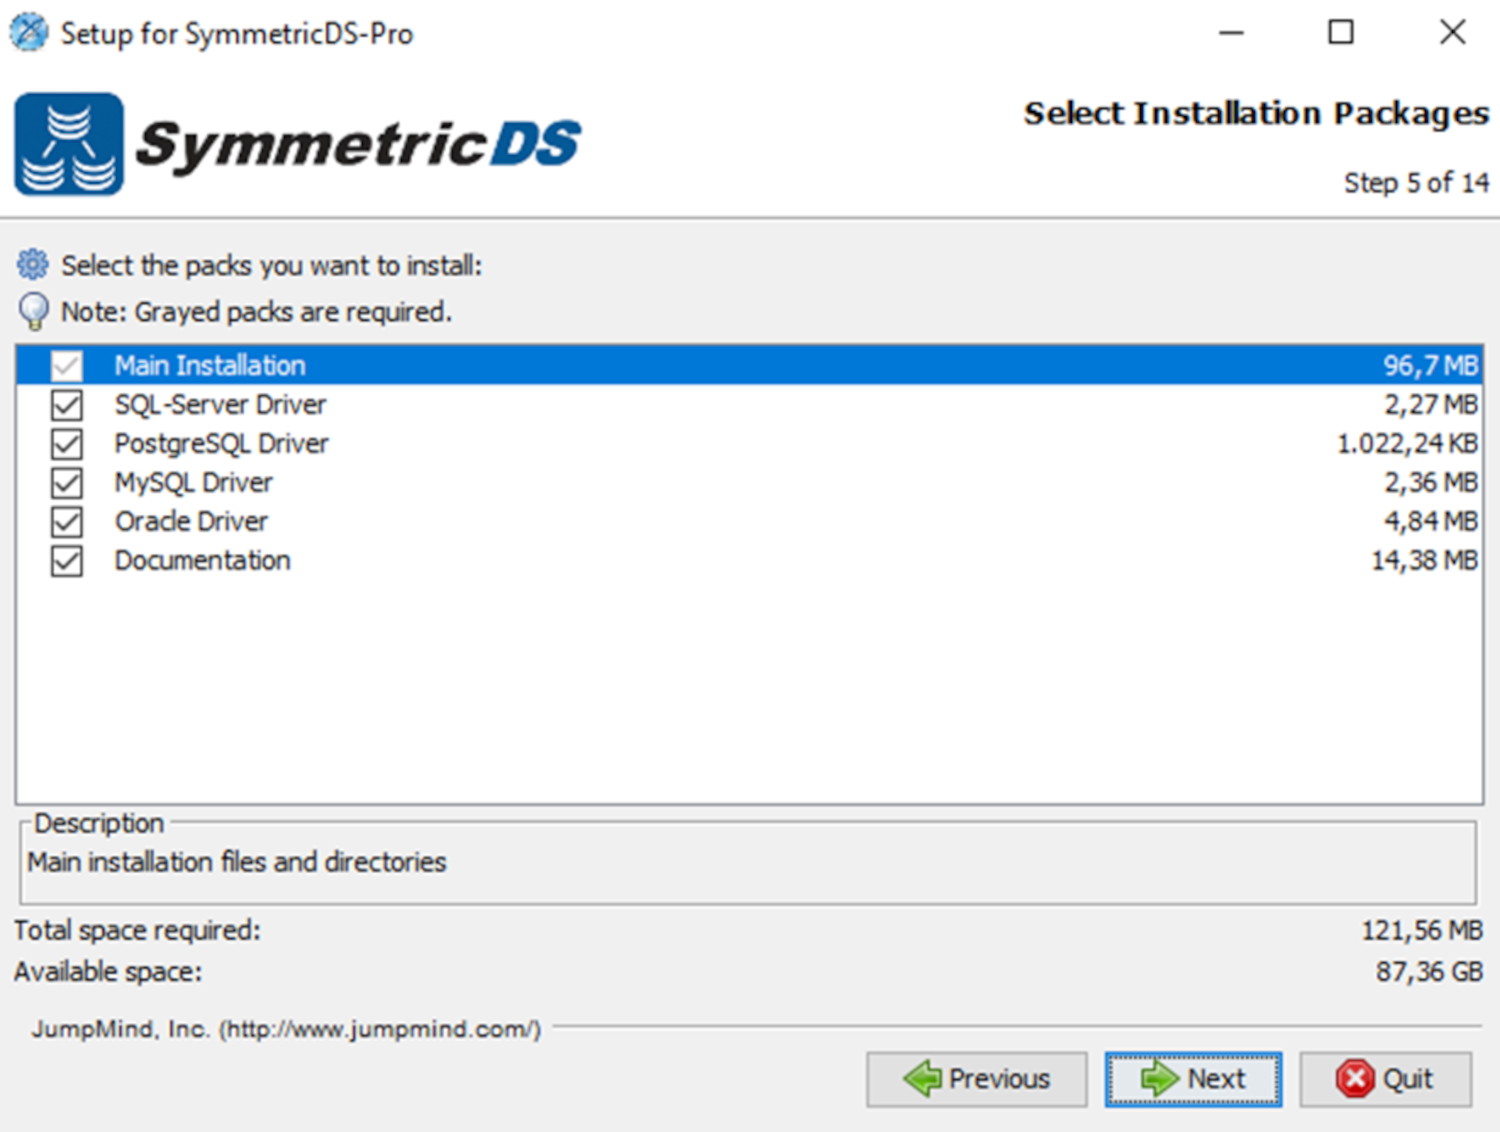
\includegraphics[width=0.5\textwidth]{SymmetricDS1.png}
	\caption{Selección de los sistemas de gestión de bases de datos con los que va a trabajar.}
	\label{fig:SymmetricDS1}
\end{figure}

SymmetricDS es un software que utiliza Internet para replicar bases de datos, por lo que requiere que se especifique el tipo de conexión y el puerto que va a utilizar. La figura \ref{fig:SymmetricDS2} muestra la ventana en la cual el usuario selecciona e ingresa estos datos.

\begin{figure}[hbt!]
	\centering
	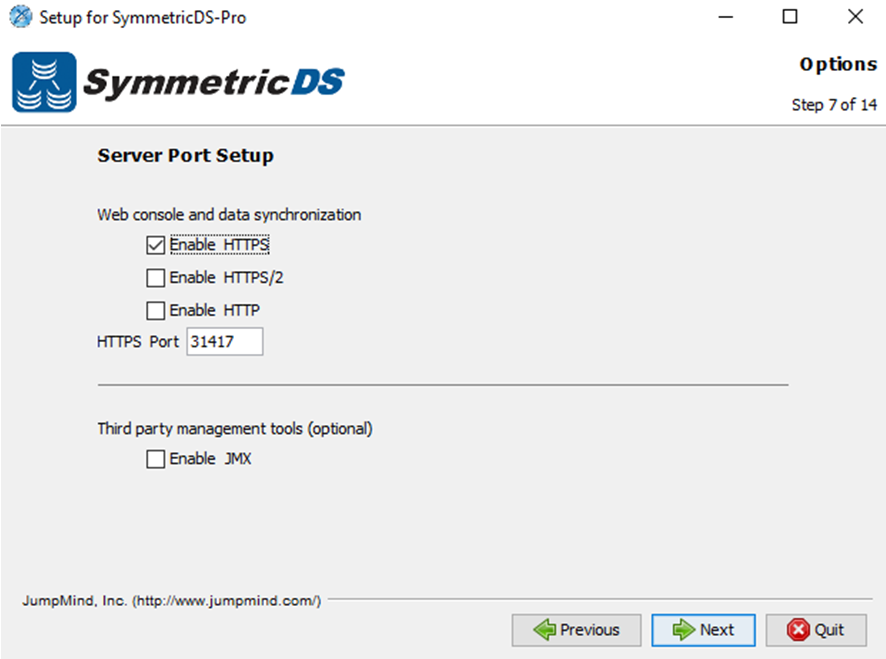
\includegraphics[width=0.5\textwidth]{SymmetricDS2.png}
	\caption{Selección del tipo de conexión y el puerto a utilizar.}
	\label{fig:SymmetricDS2}
\end{figure}
En la figura \ref{fig:SymmetricDS3}, se presenta la ventana del asistente en la cual el usuario tiene la opción de especificar la cantidad de memoria destinada para el servidor.

\begin{figure}[hbt!]
	\centering
	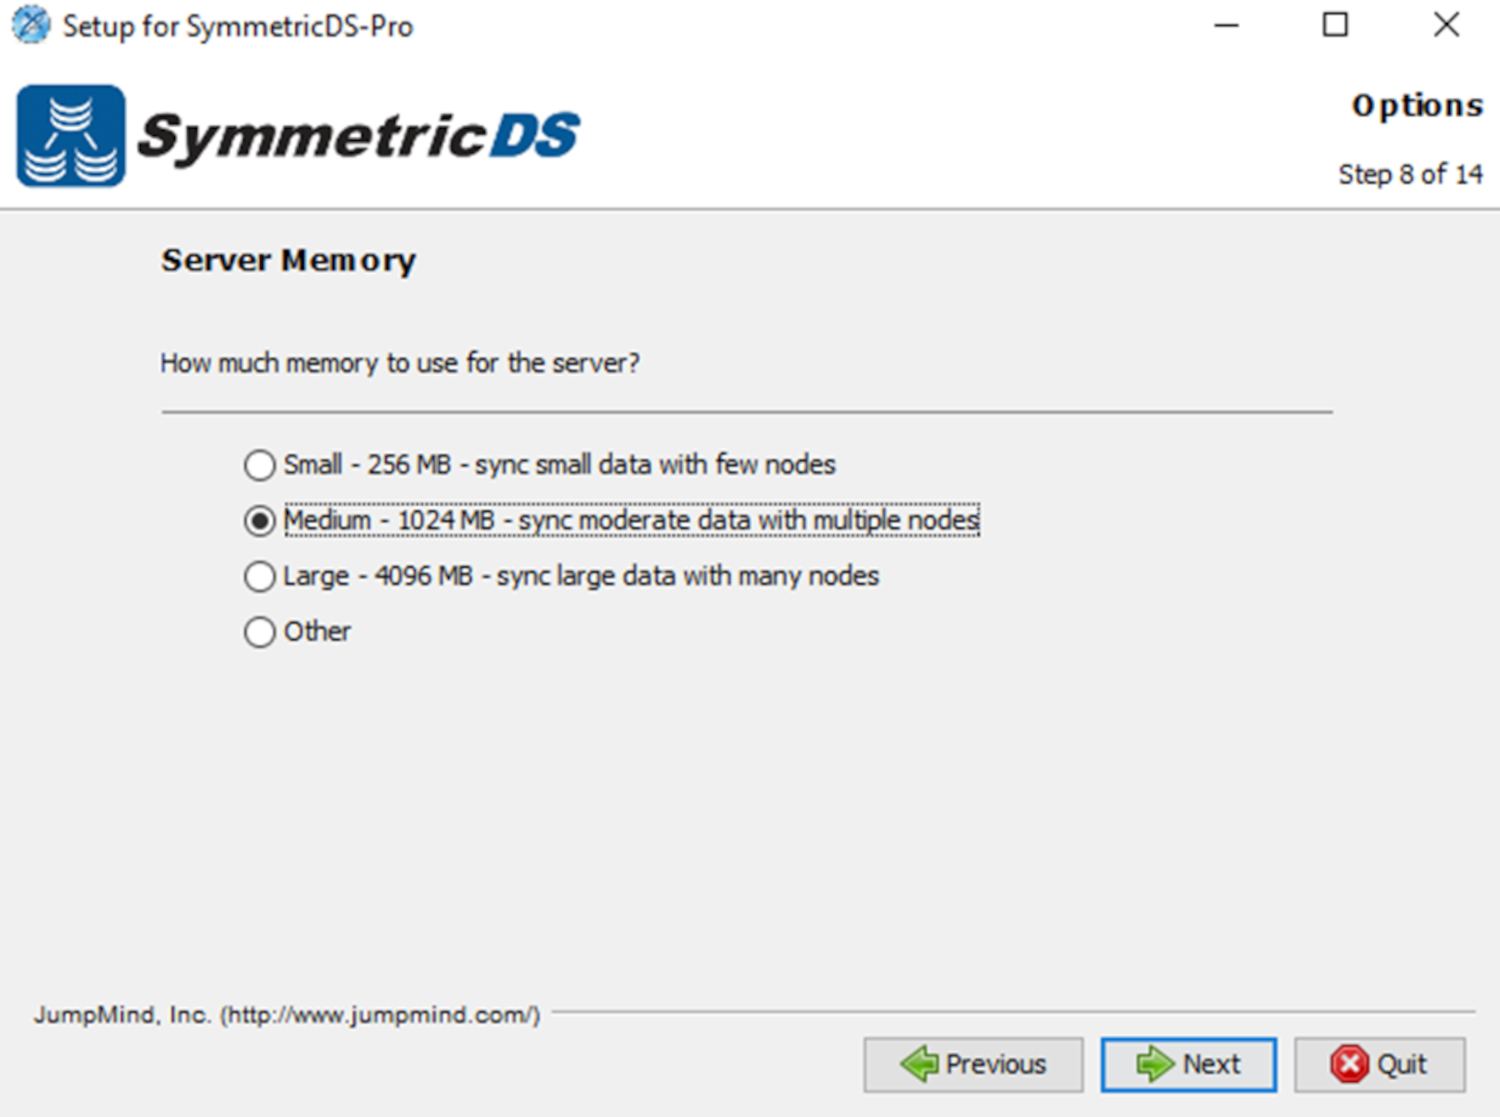
\includegraphics[width=0.5\textwidth]{SymmetricDS3.png}
	\caption{Cantidad de memoria destinada para el servidor.}
	\label{fig:SymmetricDS3}
\end{figure}

Una vez instaladas las herramientas esenciales para la replicación de bases de datos, procedemos a llevar a cabo la práctica, utilizando PostgreSQL y SQL Server. La explicación detallada de los pasos de instalación para estos gestores de bases de datos se considera innecesaria, ya que se asume que el lector tiene conocimientos previos sobre su instalación. Para involucrarse en el tema de bases de datos distribuidas, se espera que los gestores de bases de datos mencionados estén dentro del dominio del lector.

\begin{itemize}
	\item \textbf{Usando Symmetric.} Abrir SymmetricDS, y dar click en Start Server, como se muestra en la figura \ref{fig:SymmetricDS4}.
	\begin{figure}[hbt!]
		\centering
		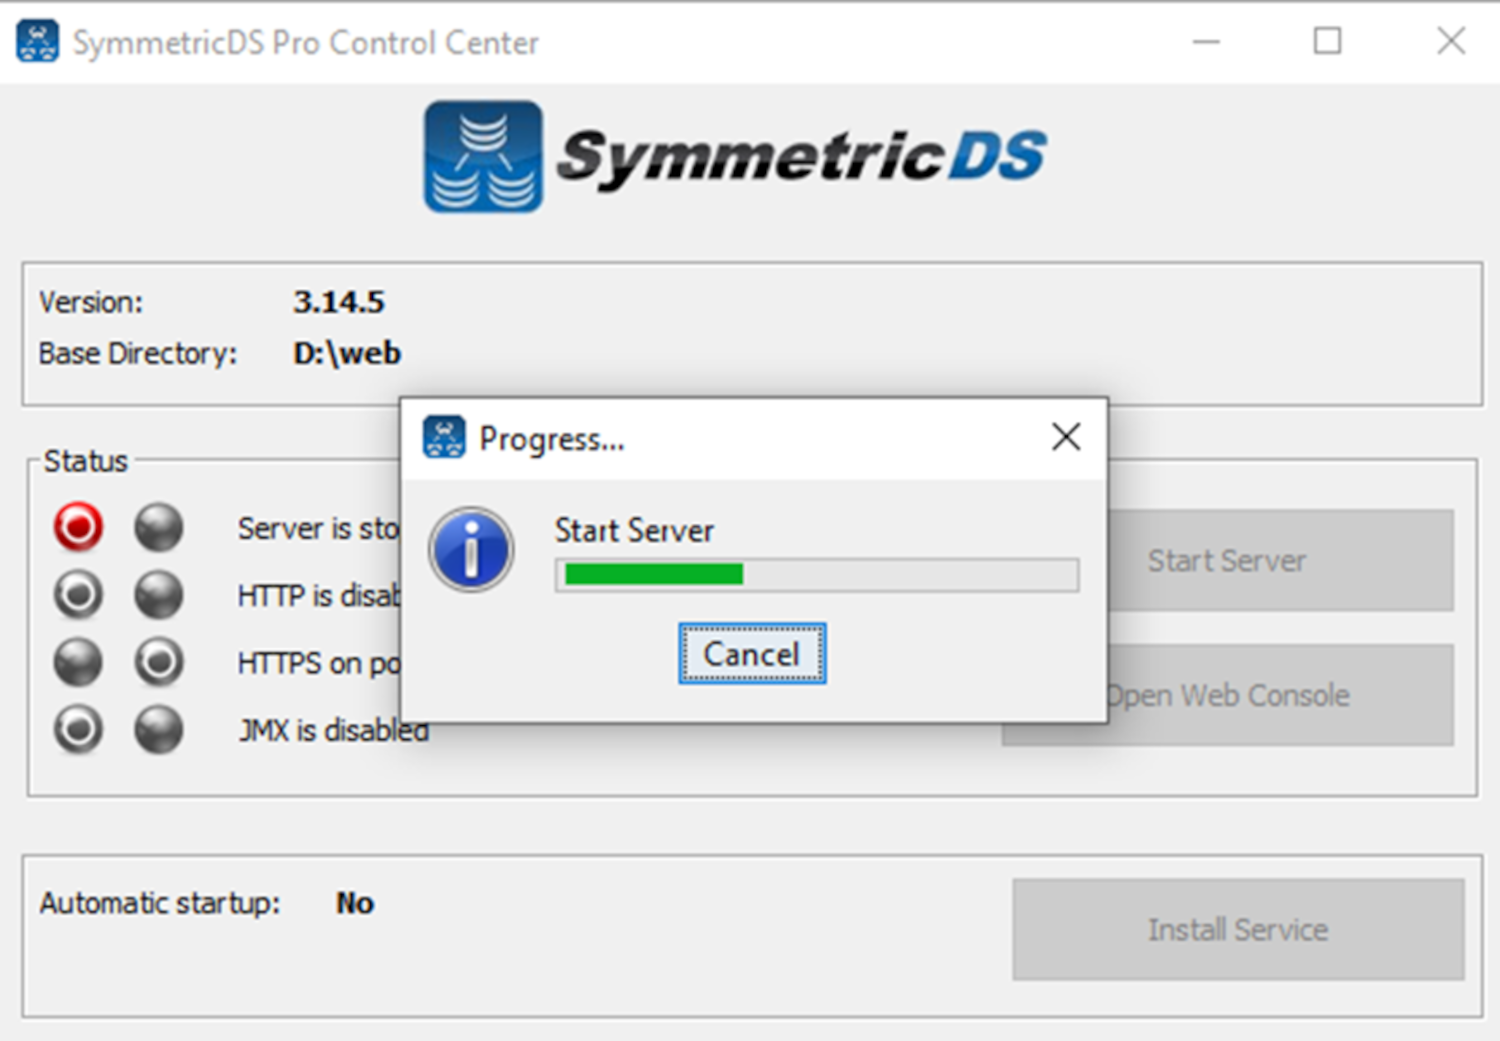
\includegraphics[width=0.5\textwidth]{SymmetricDS4.png}
		\caption{Cantidad de memoria destinada para el servidor.}
		\label{fig:SymmetricDS4}
	\end{figure}
	\item \textbf{Configuración para usar PostgreSQL:} Una vez inicializado el servidor debemos dar clic en “Open Web Console”, lo cual nos redirigirá al navegador y mostrará la pantalla que se muestra en la figura \ref{fig:SymmetricDS5}. En esa pantalla se debe seleccionar la opción de \textit{“Setup new Replication”}.
	\begin{figure}[hbt!]
		\centering
		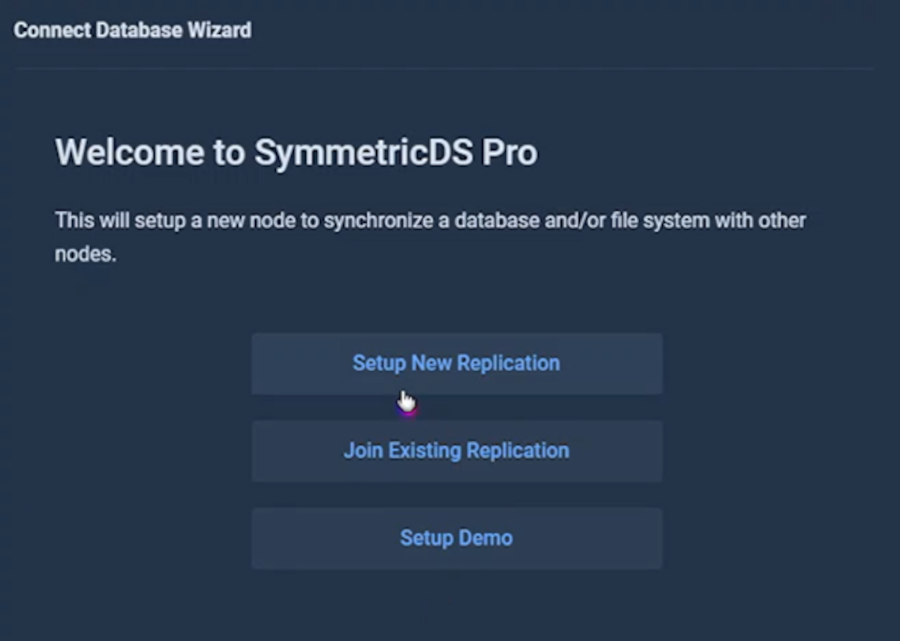
\includegraphics[width=0.5\textwidth]{SymmetricDS5.png}
		\caption{Cantidad de memoria destinada para el servidor.}
		\label{fig:SymmetricDS5}
	\end{figure}
	\item \textbf{Conexión a PostgreSQL}. En la pantalla de la figura \ref{fig:SymmetricDS6} se muestra la pestaña en la que se debe rellenar los campos con los parámetros necesarios para realizar la conexión a PostgreSQL. Para esta práctica, la base de datos se llamará “bb1”, el modo de replicación se utilizará el captura basado en Trigger (\textit{trigger-ased capture}), el user id se usará el supèr usuario “postgres\footnote{Por cuestiones de seguridad la práctica profesional hay que analizar si usar este usuario u otro.}” y la respectiva contraseña. Además de la cadena de conexión vía JBDC\footnote{Java Data Base Connectivity}, y con esto, está listo para dar clic en siguiente.
	\begin{figure}[hbt!]
		\centering
		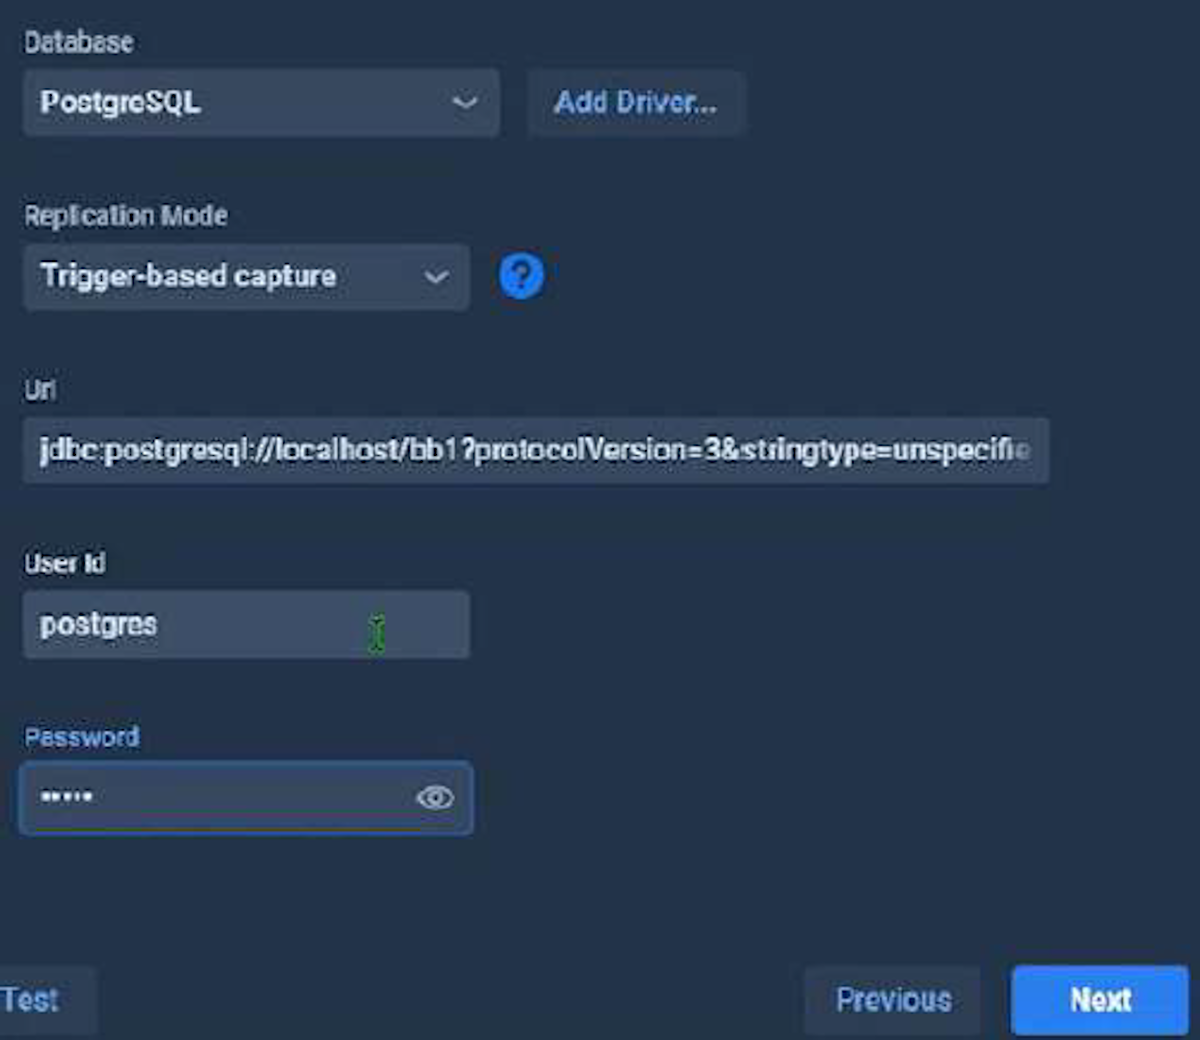
\includegraphics[width=0.5\textwidth]{images/SymmetricDS6.png}
		\caption{Parámetros para la conexión a PostgreSQL.}
		\label{fig:SymmetricDS6}
	\end{figure}
	Si los datos son correctos, la siguiente ventana mostrará el status todo yes y un visto indicando que todo se dió satisfactoriamente, a lo que debemos dar en \textit{next}, o caso contrario corregir los errores cometidos.
	\item \textbf{Tipo de replicación.} En este momento, está listo para seleccionar como será la replicación, esta ocasión como se quiere que sea de manera bidireccional, seleccionamos a la opción de “Secundary” y
	damos clic a \textit{next}.
	\item \textbf{Tipo de nodo.} Ahora se debe crear un nuevo nodo. Este nodo debe ser creado como primario. Al dar \textit{next}
	\item \textbf{Nombre del nodo.} En este paso se le debe asignar un nombre al nodo que se está creando. No es un nombre en particular, en este caso se le ha asignado el nombre de \textit{ndpg4}. Una vez asignado el nombre se da clic en \textit{next}.
	\item \textbf{Clave de la licencia.} En este momento se ingresa la licencia que debe haber llegado al correo
	electrónico, que generalmente es en un archivo de texto. El asistente muestra dos ocpiones para proporcionar la licencia como se muestra en la figura \ref{fig:SymmetricDS7}.
	
	\begin{figure}[hbt!]
		\centering
		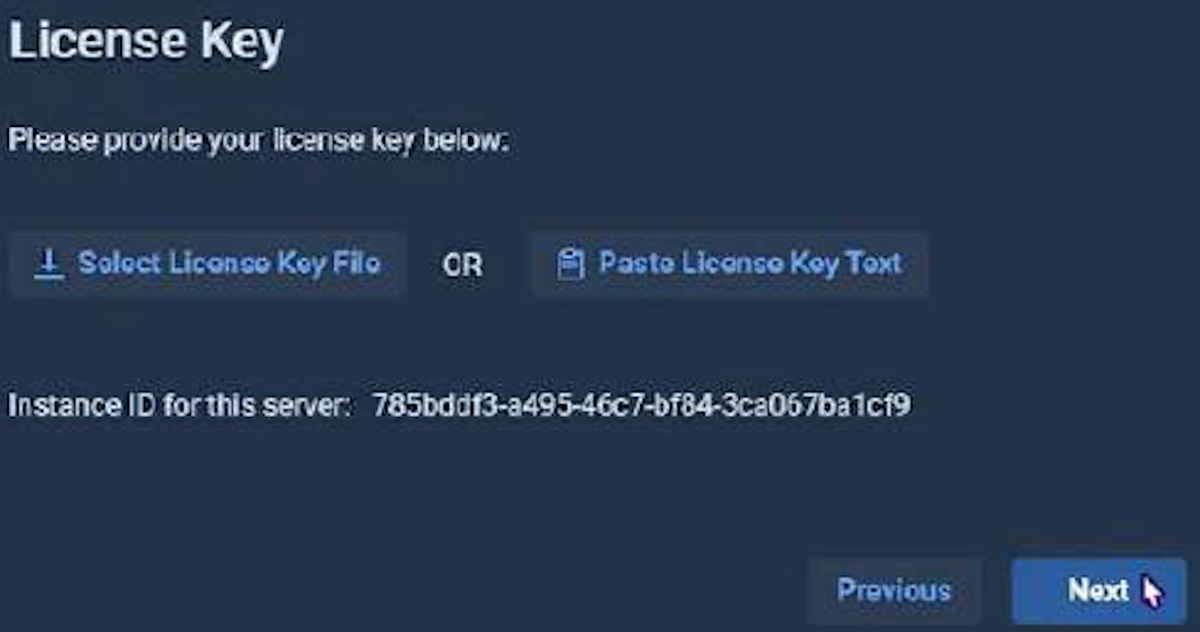
\includegraphics[width=0.5\textwidth]{images/SymmetricDS7.png}
		\caption{Proporcionar la licencia de SymmetricDS.}
		\label{fig:SymmetricDS7}
	\end{figure}
	\item \textbf{Credenciales para acceso al nodo.} Al dar clic en \textit{next}, nos mostrará la pantalla donde deberemos asignar una contraseña al user, que por defecto es admin, este nos permitirá acceder al nodo (desde consola).
	El asistente permite conocer la fortaleza de las credenciales que se está configurando, somo se muestra en la figura \ref{fig:SymmetricDS8}.
	\begin{figure}[hbt!]
		\centering
		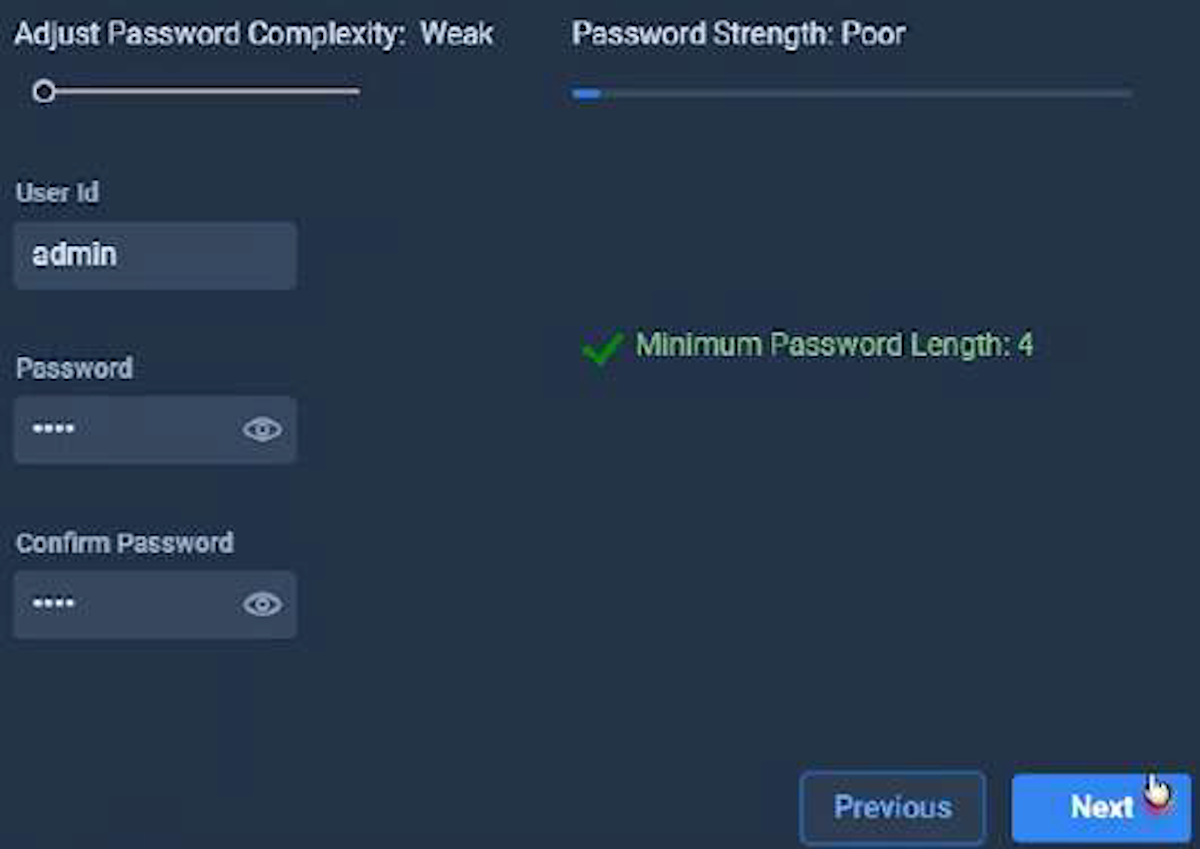
\includegraphics[width=0.5\textwidth]{images/SymmetricDS8.png}
		\caption{Credenciales de acceso al nodo.}
		\label{fig:SymmetricDS8}
	\end{figure}
	\item \textbf{Fin.} Al dar clic en \textit{next}, el asistente ha terminado de solicitar los datos para la instalación de SymmetricDS.
\end{itemize}
Una vez instalado el nodo, solicitará que se inicie sesión con las credenciales que se especificaron anteriormente (ver figura \ref{fig:SymmetricDS9}).

\begin{figure}[hbt!]
	\centering
	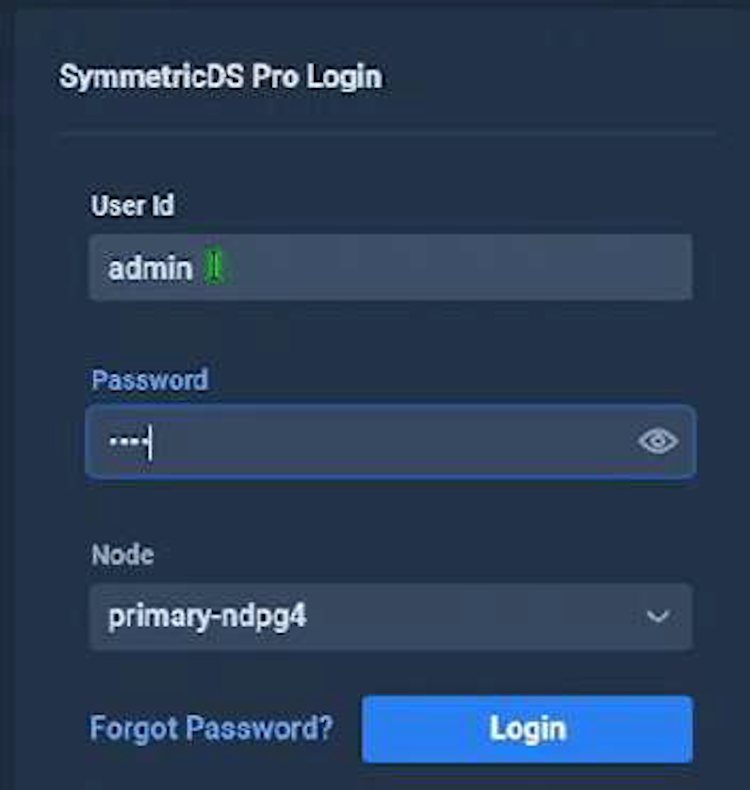
\includegraphics[width=0.35\textwidth]{images/SymmetricDS9.png}
	\caption{Inicio de sesión.}
	\label{fig:SymmetricDS9}
\end{figure}
Una vez que se inicia sesión, la misma aplicación mostrará que no existe una base de datos secundaria. Por lo tanto, se debe agregar una. En este caso se ha planeado trabajar con SQL Server. Se inicia su configuración dando clic en \textit{next}.

La configuración del nodo secundario, en este caso un servidor SQL Server, es muy similar a como se configuró en nodo primario o PostgreSQL (ver figura \ref{fig:SymmetricDS10}). Lo que se debe tener en cuenta que se seleccione el DBMS como SQL Server, la cadena de conexión, las credenciales de acceso (ver figure \ref{fig:SymmetricDS10a}), el tipo de nodo como nodo \textit{Secundary} (ver figura \ref{fig:SymmetricDS10b}), y finalmente está listo para configurar el nodo \ref{fig:SymmetricDS10c}.

\begin{figure}[htb!]
	\centering
	\begin{subfigure}{0.32\textwidth}
		\centering
		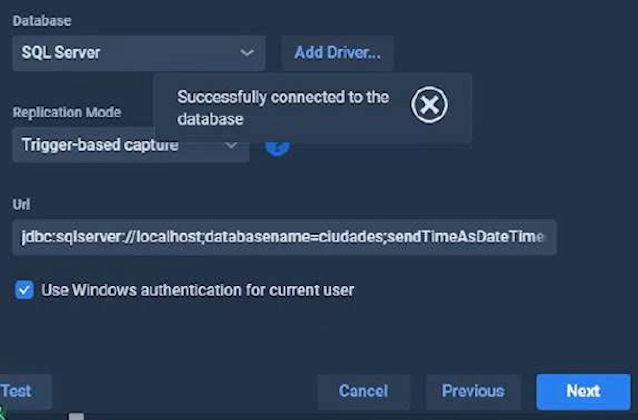
\includegraphics[height=1.45in]{SymmetricDS10a.png}
		\caption{Configurar SQL Server}
		\label{fig:SymmetricDS10a}
	\end{subfigure}
	\hfill
	\begin{subfigure}{0.32\textwidth}
		\centering
		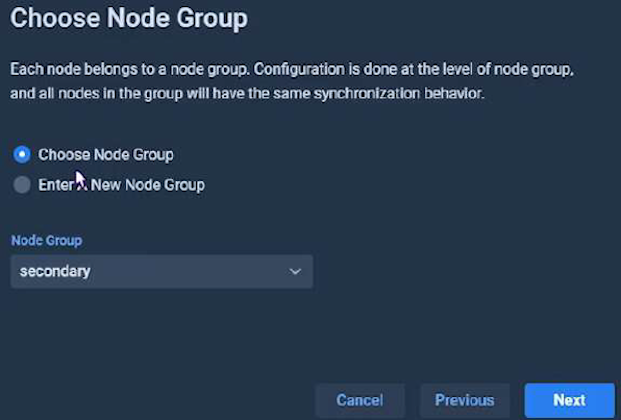
\includegraphics[height=1.45in]{SymmetricDS10b.png}
		\caption{Selección del tipo de nodo}
		\label{fig:SymmetricDS10b}
	\end{subfigure}
	\hfill
	\begin{subfigure}{0.32\textwidth}
		\centering
		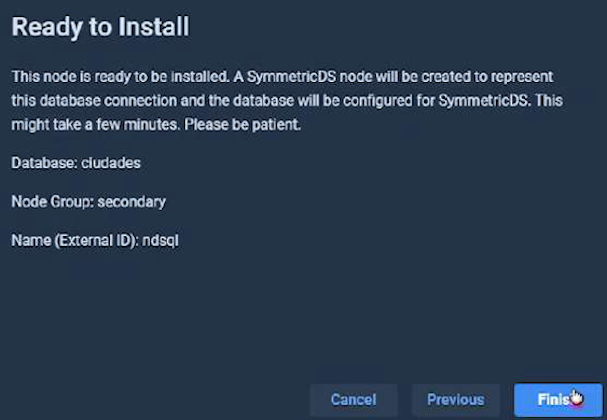
\includegraphics[height=1.45in]{SymmetricDS10c.png}
		\caption{Todo listo para instalar}
		\label{fig:SymmetricDS10c}
	\end{subfigure}
	
	\caption{Configuración de SQL Server como nodo secundario}
	\label{fig:SymmetricDS10}
\end{figure}

En el caso que se está ilustrando, el asistente informa al usuario que no ha configurado ninguna tabla para la replicación, mostrando el número de tablas existentes en las bases de datos en los dos DBMS configurados (primario y secundario). En el siguiente paso aún no se seleccionará la(s) tabla(s) con la(s) que se va a trabajar. Sin embargo, el asistente permitirá seleccionare la dirección de la replicación, es decir de nodo principal a secundario, o de secundario a principal como se muestra en la figura \ref{fig:SymmetricDS11a}. Dando clic en \textit{next}, entonces el asistente le mostrará la interfaz de la figura \ref{fig:SymmetricDS11b} para que el usuario seleccione las diferentes tablas para la replicación de datos.

\begin{figure}[htb!]
	\centering
	\begin{subfigure}{0.48\textwidth}
		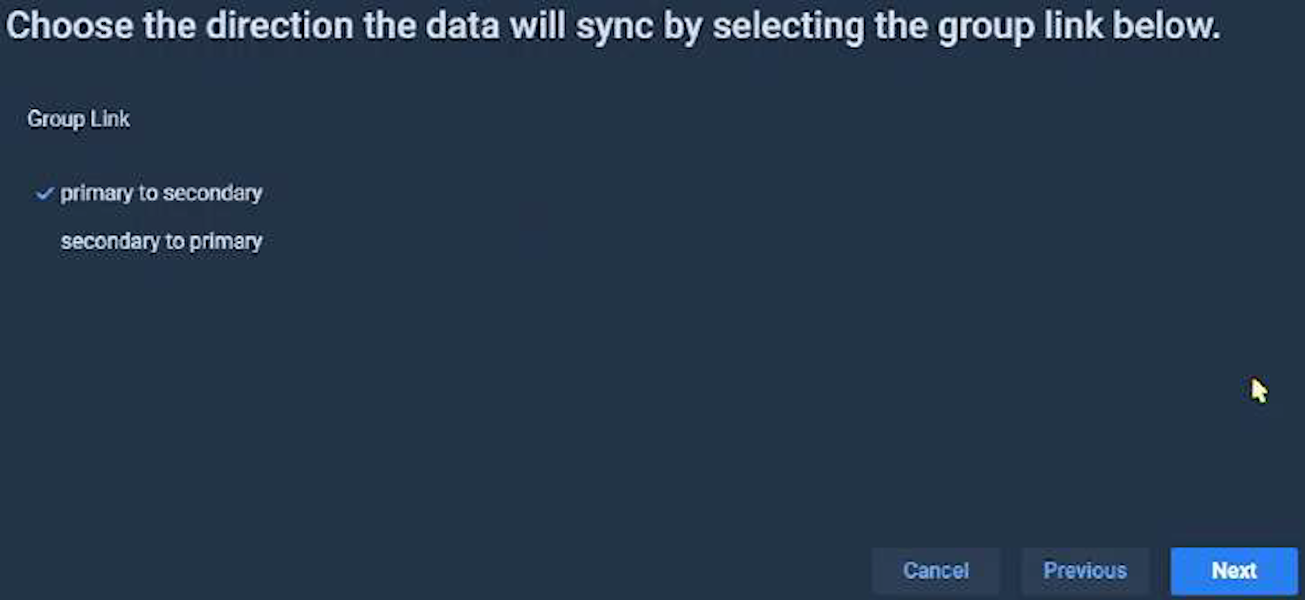
\includegraphics[height=1.5in]{SymmetricDS11a.png}
		\caption{Dirección de la replicación}
		\label{fig:SymmetricDS11a}
	\end{subfigure}
	\hfill
	\begin{subfigure}{0.48\textwidth}
		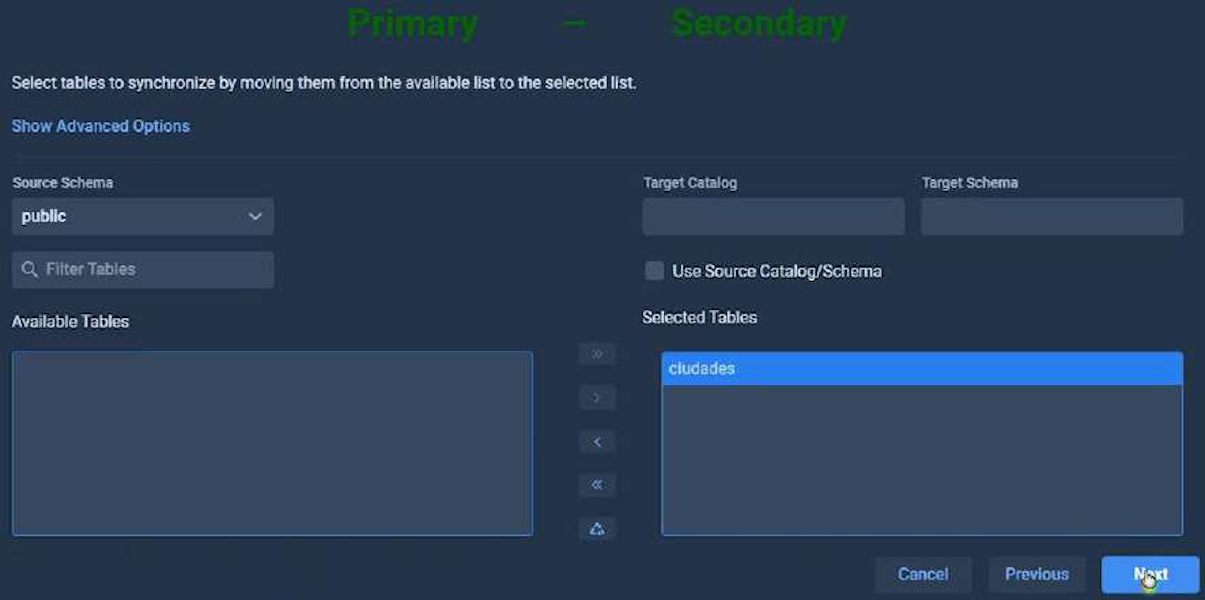
\includegraphics[height=1.5in]{SymmetricDS11b.png}
		\caption{Selección del tipo de nodo}
		\label{fig:SymmetricDS11b}
	\end{subfigure}
	\hfill
	\caption{Selección de las tablas}
	\label{fig:SymmetricDS11}
\end{figure}

Ahora bien, el asistente permitirá seleccionar la(s) base(s) de datos que recibirá(n) los datos (ver \ref{fig:SymmetricDS12}). Primero el asistente preguntará la dirección de la replicación, en una dirección o en ambas direcciones como se muestra en la figura \ref{fig:SymmetricDS12a}, para el caso práctico que se intenta ilustrar se seleccionará bidireccional. El siguiente paso cuya interfaz se muestra en la figura \ref{fig:SymmetricDS12b}, que sirve para seleccionar los nodos y bases de datos que recibirán los datos replicados.

\begin{figure}[htb!]
	\centering
	\begin{subfigure}{0.35\textwidth}
		\centering
		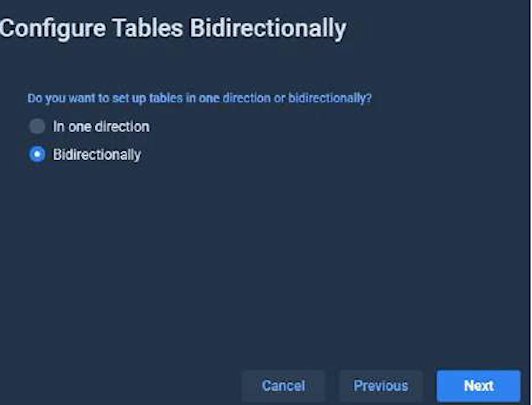
\includegraphics[height=1.65in]{SymmetricDS12a.png}
		\caption{Dirección de la replicación}
		\label{fig:SymmetricDS12a}
	\end{subfigure}
	\hfill
	\begin{subfigure}{0.63\textwidth}
		\centering
		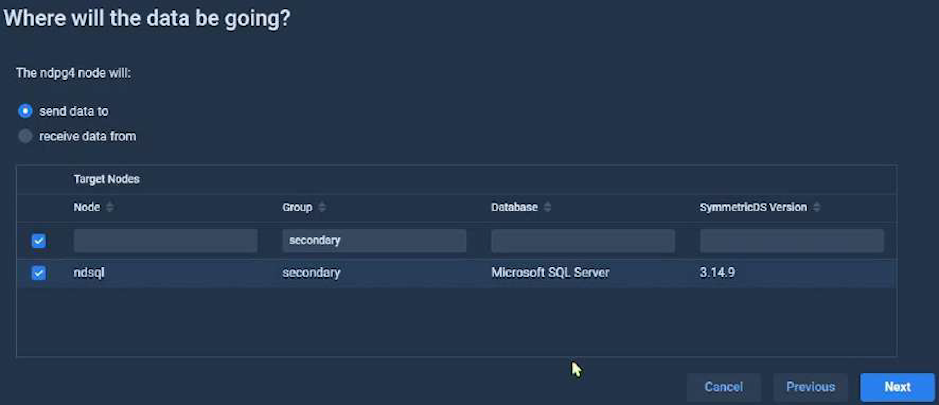
\includegraphics[height=1.65in]{SymmetricDS12b.png}
		\caption{Selección del tipo de nodo}
		\label{fig:SymmetricDS12b}
	\end{subfigure}
	\hfill
	\caption{Selección de las bases de datos de los nodos}
	\label{fig:SymmetricDS12}
\end{figure}

Una vez que se han configurado todos los parámetros de la replicación de datos, se procede a realizar las acciones que se ejecutarán inicialmente en la réplica de datos. En la figura \ref{fig:SymmetricDS13a} muestra la interfaz para seleccionar el criterio para la carga de datos de está replicación. Entre esas acciones se pueden establecer: Que tablas se cargarán (todas, especificar ciertas tablas, o según el canal). Mientras que en la figura \ref{fig:SymmetricDS13b} muestra un resumen de la carga de datos que se va a realizar.

\begin{figure}[htb!]
	\centering
	\begin{subfigure}{0.48\textwidth}
		\centering
		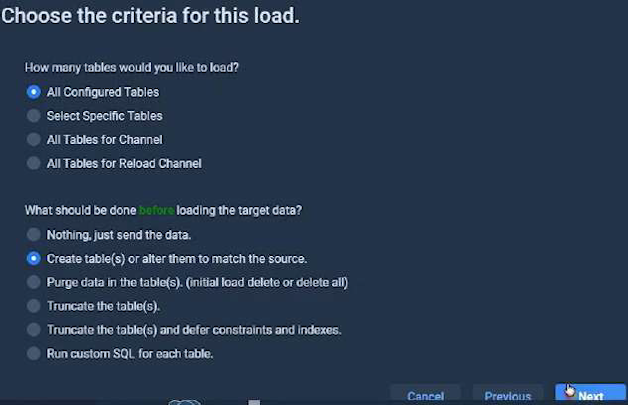
\includegraphics[height=2in]{SymmetricDS13a.png}
		\caption{Resumen de acciones de carga}
		\label{fig:SymmetricDS13a}
	\end{subfigure}
	\hfill
	\begin{subfigure}{0.48\textwidth}
		\centering
		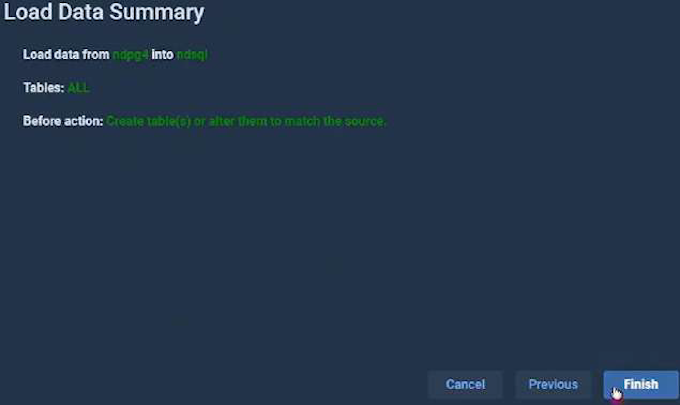
\includegraphics[height=2in]{SymmetricDS13b.png}
		\caption{Resumen de carga de datos}
		\label{fig:SymmetricDS13b}
	\end{subfigure}
	\hfill
	\caption{Carga de inicial de datos}
	\label{fig:SymmetricDS13}
\end{figure}
\noindent
Los resultados de la carga se muestran en la figura \ref{fig:SymmetricDS14}.

\begin{figure}[htb!]
	\centering
	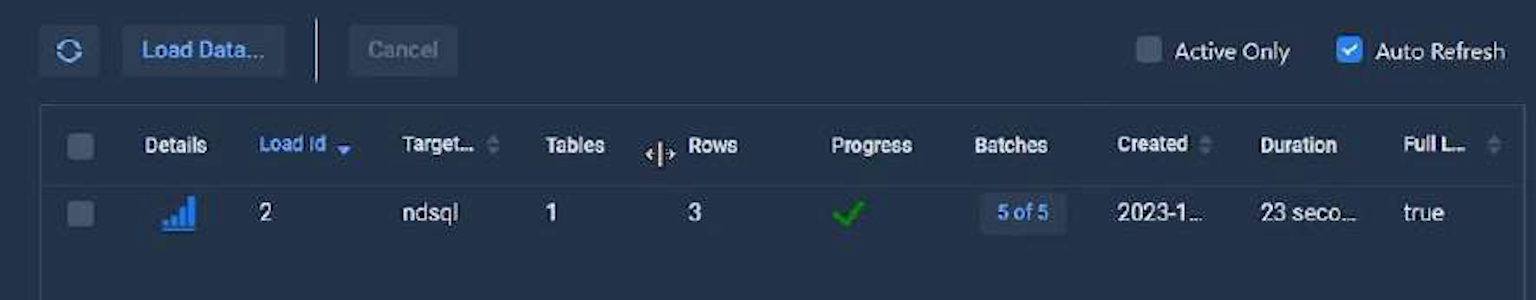
\includegraphics[width=\textwidth]{SymmetricDS14.png}
	\caption{Resultados de la carga inicial de datos}
	\label{fig:SymmetricDS14}
\end{figure}

A continuación se muestra como los datos se actualizan tanto en SQL Server como en PostgreSQL. Primero desde SQL Server se va a insertar 3 registros en la tabla de ciudades (ver listado \ref{lst:InsertInto}).

\begin{lstlisting}[language=SQL, caption={Insertar varias ciudades} \label{lst:InsertInto}]
INSERT INTO ciudades (nombre)
	VALUES ('Quito'),
	('Guayaquil'),
	('El Empalme');
\end{lstlisting}

Ahora se insertarán tres ciudades más en la misma tabla, así mismo desde SQL Server (ver listado \ref{lst:InsertIntoMas}).

\begin{lstlisting}[language=SQL, caption={Insertar múltiples ciudades}\label{lst:InsertIntoMas}]
INSERT INTO ciudades (nombre)
	VALUES ('Quioto'),
	('Guajayaquil'),
	('El Empallme');
\end{lstlisting}

\noindent
En la figura \ref{fig:SymmetricDS15} se muestra los dos momentos de la inserción de datos. Es decir después de la ejecución de las dos sentencias.

\begin{figure}[htb!]
	\centering
	\begin{subfigure}{0.48\textwidth}
		\centering
		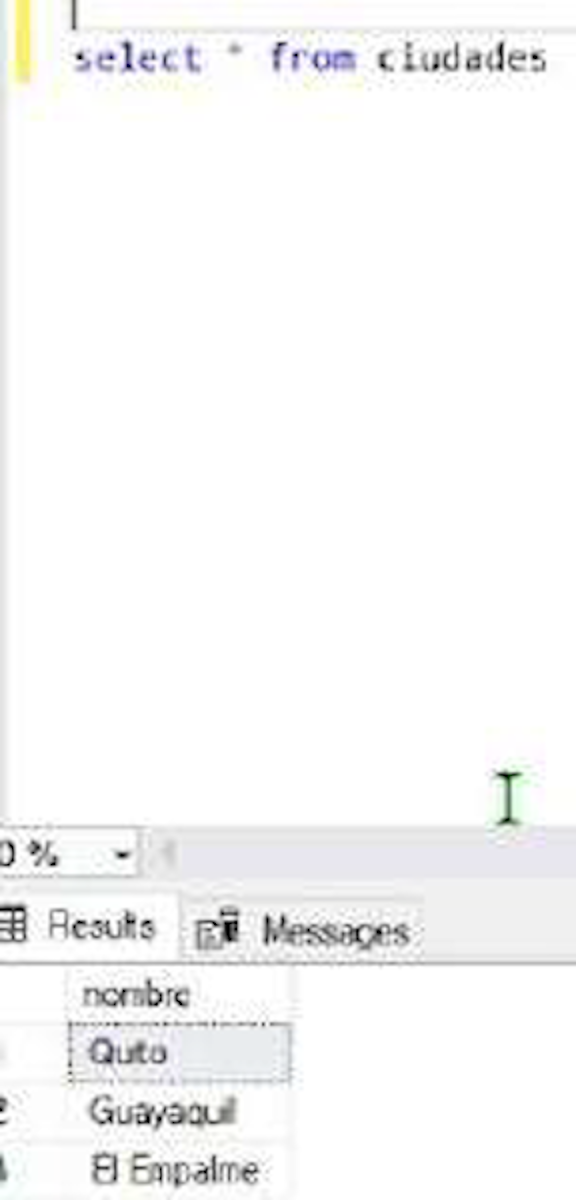
\includegraphics[height=2in]{SymmetricDS15a.png}
		\caption{Al insertar los 3 registros.}
		\label{fig:SymmetricDS15a}
	\end{subfigure}
	\hfill
	\begin{subfigure}{0.48\textwidth}
		\centering
		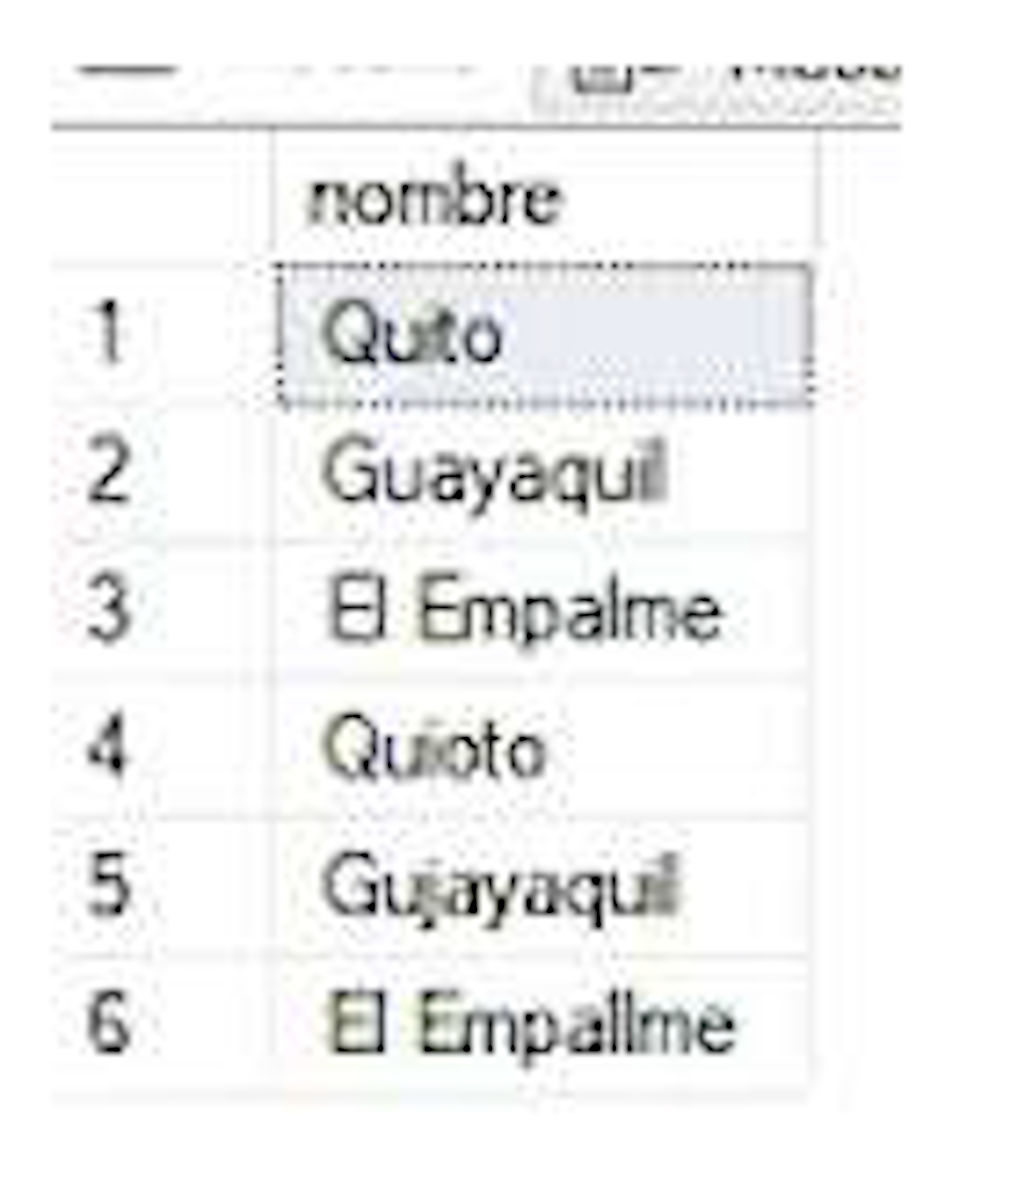
\includegraphics[height=2in]{SymmetricDS15b.png}
		\caption{Al insertar los otros 3 registros.}
		\label{fig:SymmetricDS15b}
	\end{subfigure}
	\hfill
	\caption{Resultados al Insertar datos desde SQL Server}
	\label{fig:SymmetricDS15}
\end{figure}
Si todo se realizó de manera correcta, en la pestaña del Dashboard en la consola se mostrará una pantalla como en la figure \ref{fig:SymmetricDS16}. En la cual se muestra la información de las estadísticas sobre la ejecución de los procesos (inserciones). Se debe considerar que, este proceso puede llegar a tardar algún tiempo según la cantidad de información que se ingrese.

\begin{figure}[htb!]
	\centering
	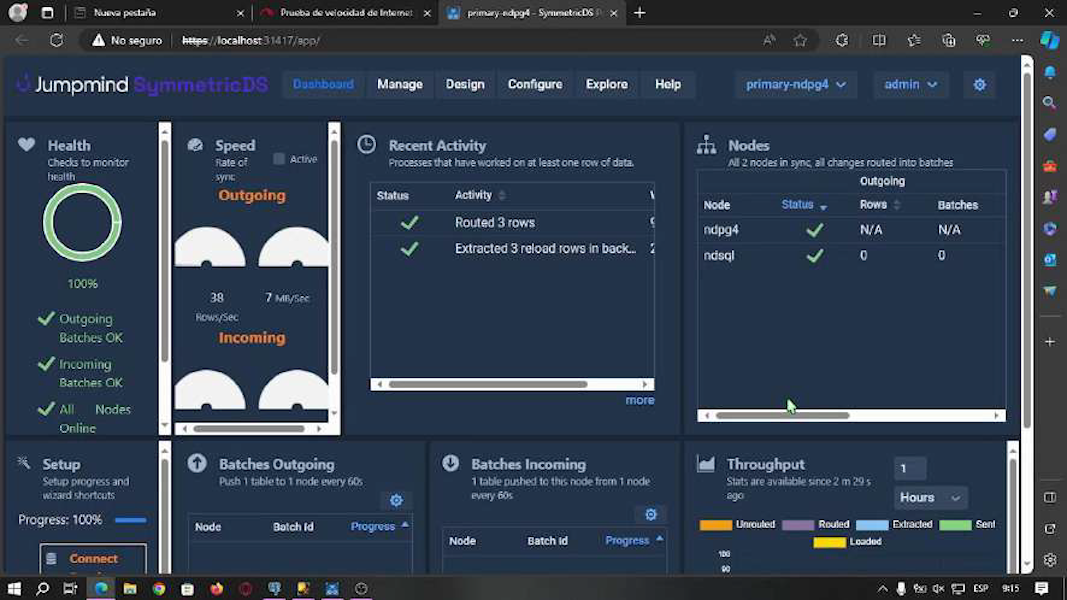
\includegraphics[width=\textwidth]{SymmetricDS16.png}
	\caption{Dashboard con la información de las estadísticas sobre la ejecución de los procesos}
	\label{fig:SymmetricDS16}
\end{figure}

Estos datos por ser replicación bidireccional, los mismos estarán en la base de datos de PostgreSQL, y si actualizamos la tabla, los datos que se ingresaron en SQL Server se ven reflejados como se muestra en la figura \ref{fig:SymmetricDS17}

\begin{figure}[htb!]
	\centering
	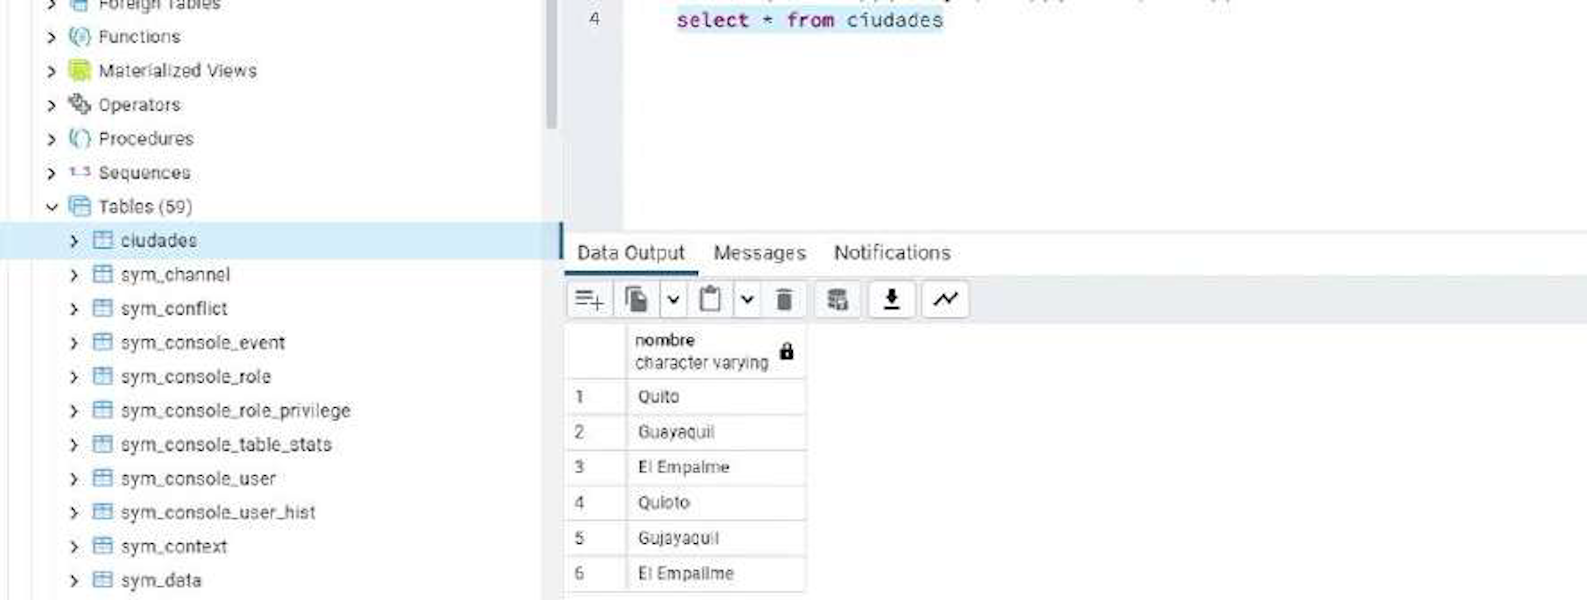
\includegraphics[width=\textwidth]{SymmetricDS17.png}
	\caption{Datos en la tabla}
	\label{fig:SymmetricDS17}
\end{figure}

Ahora se procede a realizar las inserciones desde PostGreSQL, para comprobar la bidireccionalidad.

\begin{lstlisting}[language=SQL, caption={Insertar ciudades con nombres que contienen números}]
INSERT INTO ciudades (nombre)
	VALUES ('11Quito'),
	('1Guayaquil'),
	('E1l Empalme');
\end{lstlisting}

Ahora al abrir el Dashboard en la consola web se puede observar en la figura \ref{fig:SymmetricDS18} como esta cargando.

\begin{figure}[htb!]
	\centering
	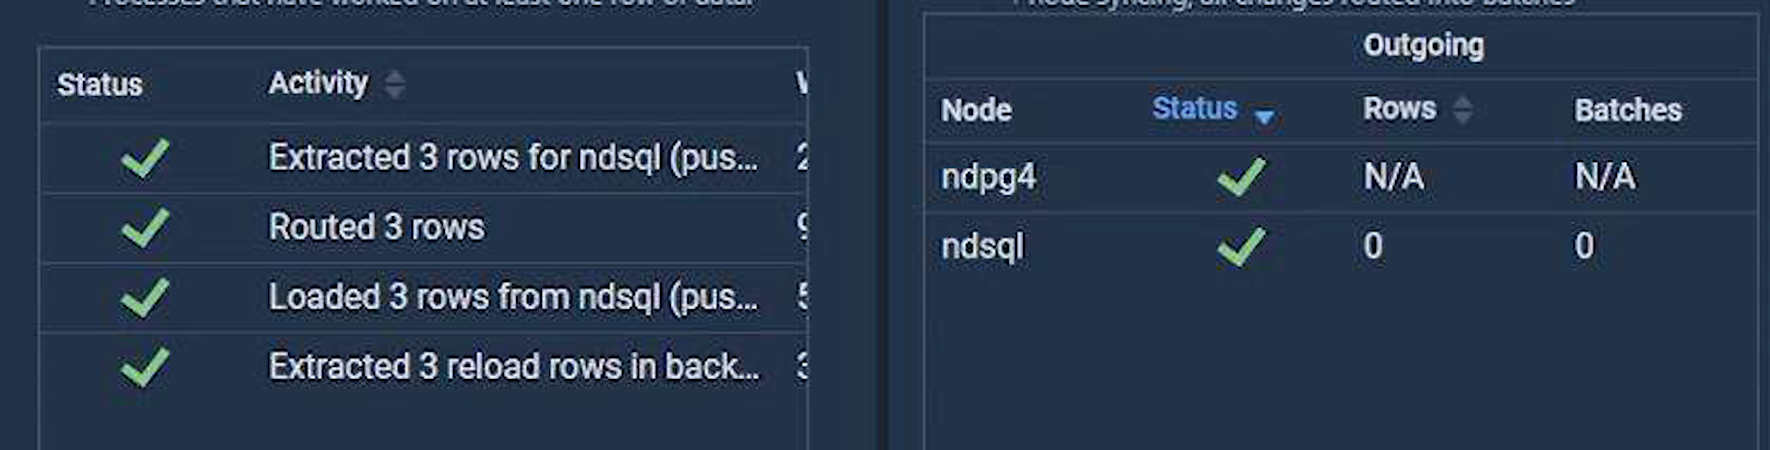
\includegraphics[width=\textwidth]{SymmetricDS18.png}
	\caption{Dashboard visualizando él éxito de las transacciones.}
	\label{fig:SymmetricDS18}
\end{figure}

Y en la captura de pantalla de la figura \ref{fig:SymmetricDS19} se muestran los datos en la tabla de la base de datos de SQL Server.

\begin{figure}[htb!]
	\centering
	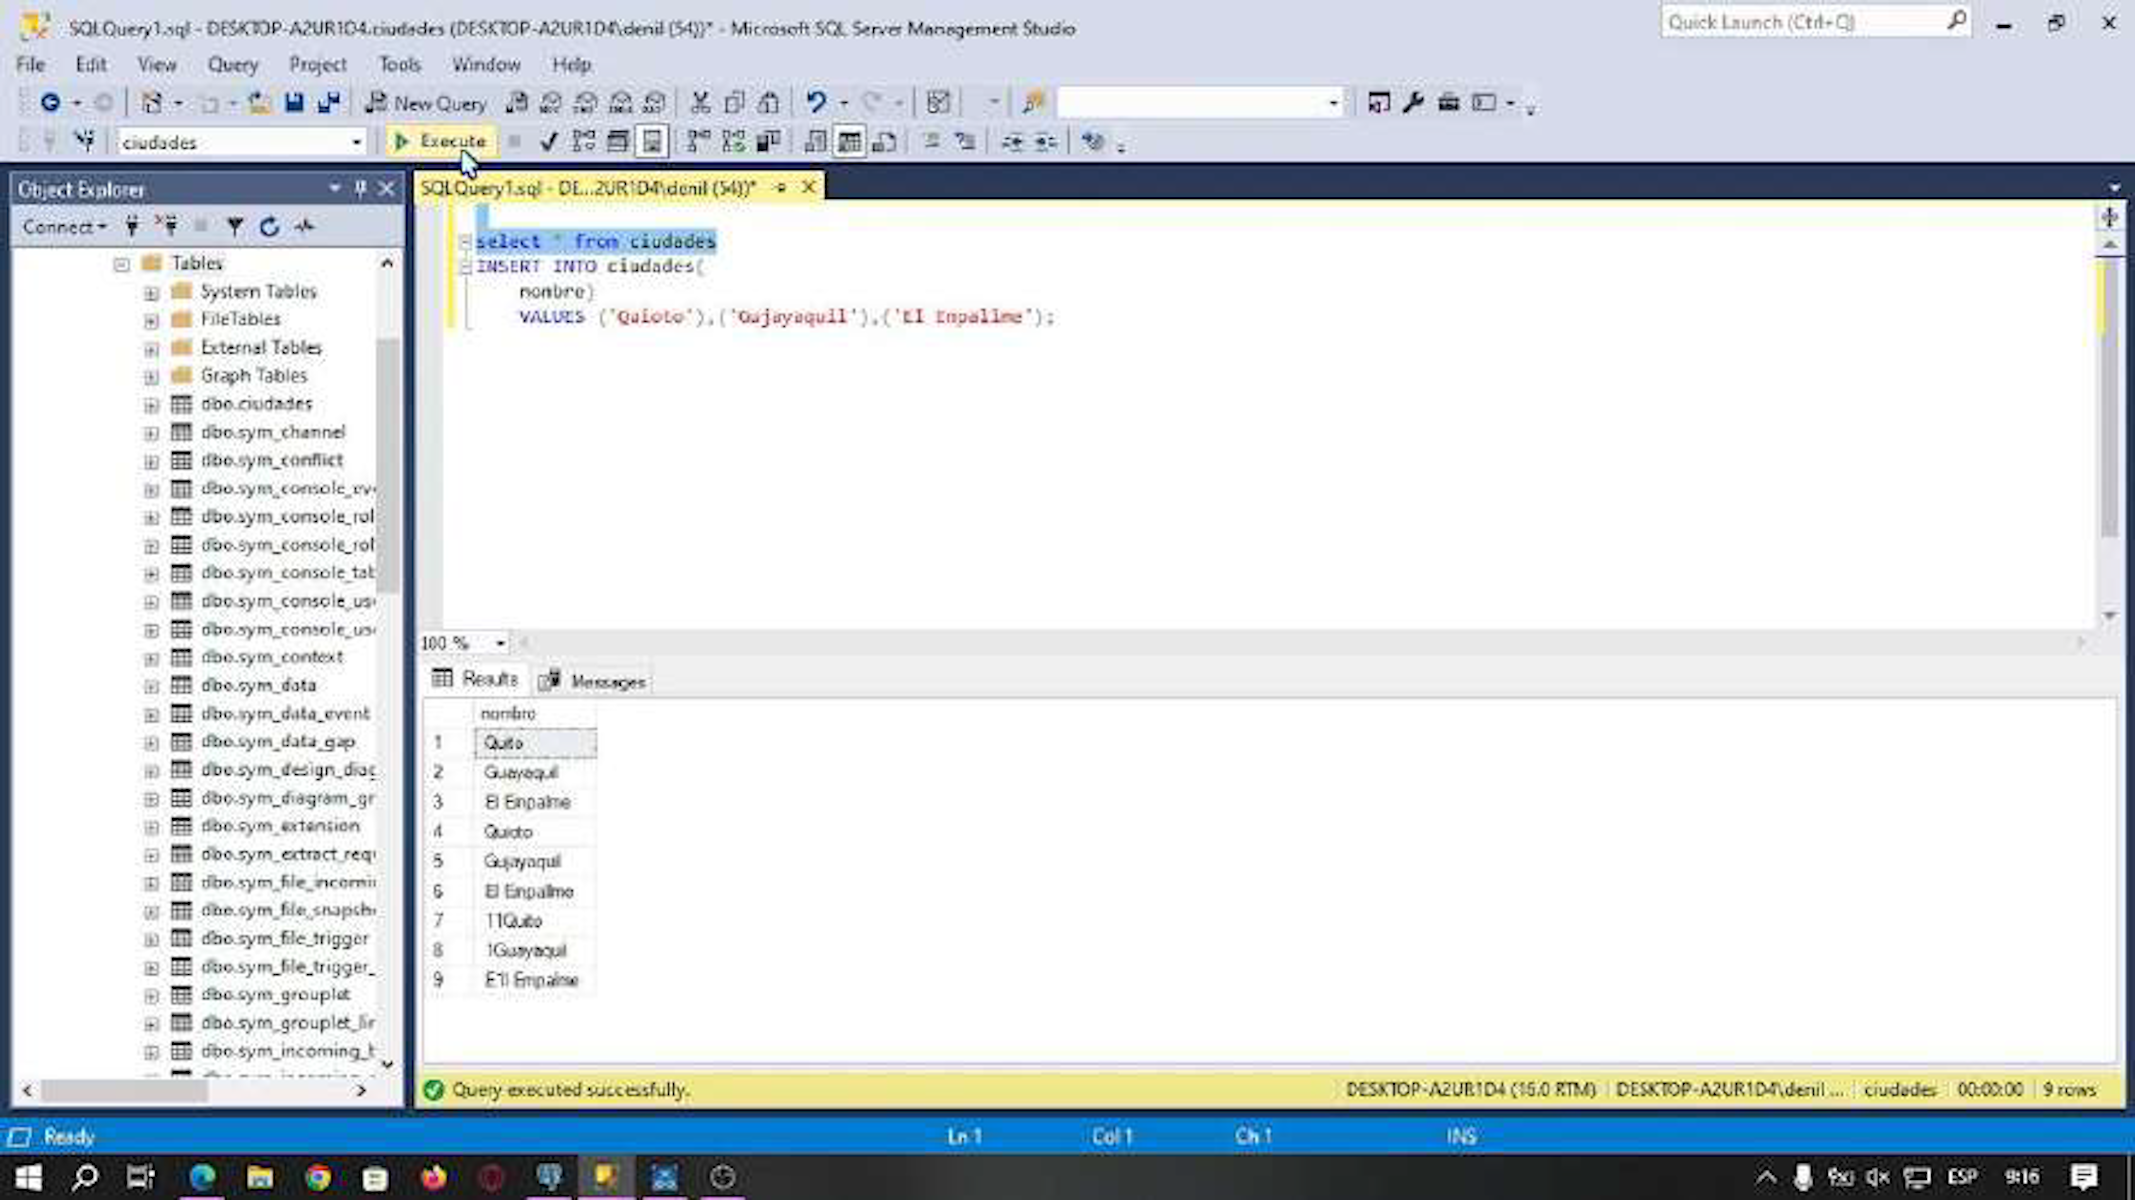
\includegraphics[width=\textwidth]{SymmetricDS19.png}
	\caption{Captura de pantalla de SQL Server con los datos actualizados.}
	\label{fig:SymmetricDS19}
\end{figure}


\subsubsection{Tolerancia a Fallos}
\noindent
En caso de un fallo en uno de los nodos de datos debido a un problema de hardware, una interrupción de red o cualquier otro motivo, el sistema sigue siendo operativo. Esto se debe a que los otros dos nodos de datos continúan funcionando y atendiendo las solicitudes de los usuarios. La tolerancia a fallos garantiza que el sistema no se vea afectado por un único punto de falla.

Además, se implementa un mecanismo de detección de fallos y conmutación por error. Si un nodo de datos se vuelve inaccesible, el sistema automáticamente redirige las solicitudes al nodo de datos más cercano disponible y actualiza la réplica del nodo fallido tan pronto como se restablezca la conectividad. Esto asegura la continuidad del servicio incluso en situaciones de fallos imprevistos.

Por lo tanto, la replicación de datos y la tolerancia a fallos en este ejemplo de base de datos distribuida garantizan que el sistema de reservas de vuelos en línea sea altamente disponible y resistente a problemas potenciales, brindando a los usuarios una experiencia confiable y sin interrupciones.

La tolerancia a fallos en los sistemas de gestión de bases de datos (DBMS) no es una propiedad intrínseca, sino más bien una característica que debe implementarse de manera consciente y específica en la arquitectura y configuración del sistema. La implementación de la tolerancia a fallos implica tomar medidas y adoptar estrategias para garantizar que el DBMS pueda continuar funcionando de manera efectiva incluso en presencia de fallos o errores inesperados.

Algunos DBMS ofrecen características y herramientas que facilitan la implementación de la tolerancia a fallos, pero aún así, es responsabilidad del administrador del sistema configurar y administrar estas características de manera adecuada. Algunas de las técnicas y características comunes utilizadas para lograr la tolerancia a fallos en sistemas de bases de datos incluyen:

\begin{enumerate}
	\item \textbf{Replicación de Datos:} Mantener copias redundantes de los datos en múltiples ubicaciones o nodos para que, en caso de fallo en un nodo, los datos estén disponibles en otros nodos.
	\item \textbf{Clustering y Alta Disponibilidad:} Utilizar configuraciones de clústeres y servidores redundantes para garantizar la disponibilidad continua del servicio en caso de fallo de hardware o software.
	\item \textbf{Copia de Seguridad y Recuperación:} Realizar copias de seguridad periódicas de los datos y tener procedimientos de recuperación en caso de pérdida de datos o fallo del sistema.
	\item \textbf{Detección de Fallos y Conmutación por Error:} Implementar sistemas de detección de fallos que alerten sobre problemas y permitan la conmutación automática a un sistema de respaldo en caso de fallo.
	\item \textbf{Tolerancia a Fallos de Red:} Considerar la redundancia de red y las rutas alternativas para garantizar la conectividad en caso de problemas de red.
	\item \textbf{Monitoreo Continuo:} Establecer sistemas de monitoreo y alerta para detectar y responder rápidamente a problemas antes de que afecten gravemente la operación.
	\item \textbf{Planificación de Capacidad:} Evitar la sobrecarga del sistema y garantizar que haya recursos suficientes disponibles para manejar situaciones de carga inesperadas.
\end{enumerate}
\begin{tcolorbox}[colback=yellow!10!white, colframe=blue!50!black, title=Resumiendo, coltitle=white]
	La tolerancia a fallos es una preocupación fundamental en la administración de bases de datos distribuidas y sistemas de gestión de bases de datos en general. Aunque algunos DBMS pueden ofrecer características específicas para facilitar la tolerancia a fallos, su implementación y gestión efectivas requieren la planificación y la adopción de estrategias adecuadas por parte de los administradores de sistemas y bases de datos.
\end{tcolorbox}

\subsection{Fragmentación}
\noindent
La fragmentación es el proceso de dividir una base de datos en fragmentos o particiones más pequeñas que se almacenan en diferentes nodos. Cada fragmento contiene un subconjunto de los datos totales y la fragmentación puede ser horizontal (por filas) o vertical (por columnas) dependiendo de cómo se dividan los datos.
\begin{itemize}
	\item \textbf{Fragmentación horizontal:} La fragmentación horizontal es un enfoque de fragmentación en el cual las filas de una tabla se dividen y distribuyen en diferentes nodos. Cada nodo contendrá un subconjunto de filas, lo que permite una distribución equilibrada de los datos.
	\item \textbf{Fragmentación vertical:} La fragmentación vertical es un enfoque de fragmentación en el cual las columnas de una tabla se dividen y distribuyen en diferentes nodos. Cada nodo contendrá un subconjunto de columnas, lo que permite una distribución eficiente de los datos según las necesidades de acceso y rendimiento.
\end{itemize}

\subsubsection{Fragmentación Vertical en PostgreSQL:}
\noindent
La fragmentación vertical implica dividir una tabla en columnas, de modo que cada fragmento contenga un subconjunto diferente de columnas. Esto es útil cuando se desea distribuir las columnas de una tabla en diferentes nodos o servidores según sus necesidades. Aquí hay un ejemplo:

Si se estuviese gestionando una base de datos distribuida para una empresa de comercio electrónico que vende productos en línea. Se tiene una tabla llamada "Productos" que contiene información sobre los productos, incluyendo detalles como el nombre, la descripción, el precio y la disponibilidad. Sin embargo, en algunos nodos de nuestra base de datos distribuida, sólo se necesita información sobre el nombre y la descripción de los productos, mientras que en otros nodos se necesita toda la información.

Se podría crear dos fragmentos de la tabla "Productos" de la siguiente manera:

Fragmento 1 (contiene solo el nombre y la descripción - listado \ref{lst:CreateSelect}). 

\begin{lstlisting}[language=SQL, caption={Crear una nueva tabla a partir de otra}\label{lst:CreateSelect}]
CREATE TABLE fragmento_productos_1 AS
	SELECT nombre, descripcion
	FROM productos;
\end{lstlisting}

Fragmento 2 (contiene todos los detalles del producto - listado \ref{lst:CreateCopyTable}).

\begin{lstlisting}[language=SQL, caption={Crear una tabla copia de productos} \label{lst:CreateCopyTable}]
CREATE TABLE fragmento_productos_2 AS
	SELECT *
	FROM productos;
\end{lstlisting}

De esta manera, los nodos que solo necesitan el nombre y la descripción de los productos pueden acceder al Fragmento 1, mientras que aquellos que requieren todos los detalles pueden acceder al Fragmento 2. Esto permite una distribución más eficiente de los datos según las necesidades de cada nodo.

\subsubsection{Fragmentación Horizontal en PostgreSQL}
\noindent
La fragmentación horizontal implica dividir una tabla en filas, de modo que cada fragmento contenga un subconjunto diferente de filas. Esto es útil cuando se desea distribuir datos de una tabla en función de un criterio específico. Aquí hay un ejemplo:

Como ejemplo se puede considerar que se está gestionando una base de datos distribuida para una cadena de tiendas minoristas en diferentes ubicaciones geográficas. Se tiene una tabla llamada "Ventas" que registra las ventas diarias en todas las tiendas. Para mejorar el rendimiento y facilitar el acceso a los datos, se decide fragmentar la tabla por ubicación geográfica.

Se podría crear fragmentos de la tabla "Ventas" de la siguiente manera:

Fragmento 1 (registros de ventas de Nueva York - listado \ref{lst:CreateTableNewYorkSales}).

\begin{lstlisting}[language=SQL, caption={Crear una tabla con ventas de Nueva York} \label{lst:CreateTableNewYorkSales}]
CREATE TABLE fragmento_ventas_ny AS
	SELECT *
	FROM ventas
	WHERE ubicacion = 'Nueva York';
\end{lstlisting}

\noindent
Fragmento 2 (registros de ventas de Los Ángeles - listado \ref{lst:CreateTableLosAngelesSales}).

\begin{lstlisting}[language=SQL, caption={Crear una tabla con ventas de Los Ángeles} \label{lst:CreateTableLosAngelesSales}]
CREATE TABLE fragmento_ventas_la AS
	SELECT *
	FROM ventas
	WHERE ubicacion = 'Los %Á%ngeles';
\end{lstlisting}

Fragmento 3 (registros de ventas de Chicago - listado \ref{lst:CreateTableChicagoSales}).

\begin{lstlisting}[language=SQL, caption={Crear una tabla con ventas de Chicago} \label{lst:CreateTableChicagoSales}]
CREATE TABLE fragmento_ventas_chicago AS
	SELECT *
	FROM ventas
	WHERE ubicacion = 'Chicago';
\end{lstlisting}

Cada fragmento contiene los registros de ventas correspondientes a una ubicación geográfica específica. Esto facilita la recuperación de datos de ventas para cada ubicación de manera eficiente y reduce la carga en los nodos de la base de datos distribuida.

\subsection{Consistencia y Coherencia de datos}
\noindent
La consistencia en una base de datos distribuida se refiere a la propiedad de que todos los nodos vean y operen con datos consistentes. Por su parte la coherencia en una base de datos distribuida se refiere a la propiedad de que todos los nodos vean una versión consistente de los datos en todo momento. Esto implica que los nodos reflejen las actualizaciones de manera ordenada y coherente para mantener la integridad de los datos.

\subsubsection{Consistencia y Coherencia de Datos en SQL Server}
\noindent
Se puede suponer que se está gestionando una base de datos distribuida para una cadena de tiendas minoristas en diferentes ubicaciones geográficas. Se tiene una tabla llamada "Inventario" que registra la cantidad de productos disponibles en cada tienda. Para garantizar la consistencia y la coherencia de datos, se requiere asegurar de que las siguientes condiciones se cumplan en todo momento:

\begin{itemize}
	\item La cantidad de productos en el inventario nunca sea negativa.
	\item Cuando se realiza una venta en una tienda, la cantidad de productos disponibles se actualice correctamente.
	\item Los cambios en el inventario se reflejen en todas las ubicaciones de manera consistente y en tiempo real.
\end{itemize}
Para lograr esto, puedes utilizar las siguientes estrategias y sentencias SQL en SQL Server:

\begin{enumerate}
	\item \textbf{Utilizar Restricciones de Integridad.} Se puede definir restricciones de integridad para garantizar que la cantidad de productos nunca sea negativa. Por ejemplo en el listado de código \ref{lst:CreateTable}:
	
	\begin{lstlisting}[language=SQL, caption={Crear tabla Inventario con restricción CHECK} \label{lst:CreateTable}]
CREATE TABLE Inventario (
	ProductoID INT PRIMARY KEY,
	Cantidad INT CHECK (Cantidad >= 0),
	Ubicacion VARCHAR(50)
);
	\end{lstlisting}
	
	La restricción CHECK (ver ejemplo \ref{lst:CreateTable}) asegura que la cantidad no sea negativa en ningún momento.
	\item \textbf{Transacciones para Actualizar el Inventario.} Cuando se realiza una venta en una tienda, se debe asegurar de que la cantidad de productos disponibles se actualice correctamente. Se puede hacer esto utilizando transacciones en SQL Server para garantizar que las operaciones sean atómicas y consistentes. Por ejemplo (\label{eje:ConCohe}):
	
	\texttt{\\BEGIN TRANSACTION;\\
		-- Restar la cantidad vendida del inventario\\
		UPDATE Inventario\\
		SET Cantidad = Cantidad - @CantidadVendida\\
		WHERE ProductoID = @ProductoID AND Ubicacion = @Ubicacion;\\ \\
		-- Registrar la venta en la tabla de ventas\\
		INSERT INTO Ventas (ProductoID, CantidadVendida, Fecha, Ubicacion) \\
		VALUES (@ProductoID, @CantidadVendida, GETDATE(), @Ubicacion);\\ \\
		COMMIT;
	}
	\item \textbf{Uso de Replicación o Distribución de Datos.} Para asegurarte de que los cambios en el inventario se reflejen en todas las ubicaciones de manera consistente y en tiempo real, puedes utilizar características de replicación o distribución de datos en SQL Server. Esto garantiza que los datos estén sincronizados en todas las ubicaciones, lo que mejora la coherencia de datos en todo el sistema.
\end{enumerate}
Estas estrategias y sentencias SQL en SQL Server son ejemplos de cómo puedes garantizar la consistencia y la coherencia de datos en una base de datos distribuida. Mantener un control estricto sobre las operaciones de actualización y utilizar restricciones de integridad son prácticas clave para mantener datos confiables y coherentes en entornos distribuidos.

\subsection{Atomicidad}
\noindent
La atomicidad se refiere a la propiedad de una operación en una base de datos distribuida de ser una unidad atómica e indivisible. Esto significa que una operación se realiza en su totalidad o no se realiza en absoluto, evitando así resultados parciales o inconsistentes (ver ejemplo \ref{eje:ConCohe}).

\subsection{Consenso}
\noindent
El consenso es un proceso en el cual los nodos de una base de datos distribuida llegan a un acuerdo sobre una decisión o valor común. Esto se logra mediante algoritmos de consenso, como el algoritmo de consenso de Paxos o el algoritmo de tolerancia a fallas bizantinas (BFT), que permiten a los nodos llegar a un consenso incluso si algunos nodos fallan o son maliciosos.

El "\textit{consenso}" en el contexto de las bases de datos distribuidas se refiere a la necesidad de garantizar que todas las réplicas de datos en diferentes nodos estén sincronizadas y reflejen la misma información, incluso en presencia de operaciones concurrentes y actualizaciones. Una técnica común para lograr el consenso es la utilización de transacciones distribuidas. A continuación, se presenta el ejemplo \ref{eje:consenso} de cómo se puede implementar el consenso con SQL Server mediante el uso de transacciones distribuidas.

Si se está gestionando una base de datos distribuida para una cadena de tiendas minoristas en diferentes ubicaciones geográficas, entonces, se desea garantizar que las ventas realizadas en cada tienda se registren de manera coherente y que los totales de ventas se actualicen correctamente en tiempo real en una base de datos centralizada. En este escenario, se puede utilizar transacciones distribuidas para lograr el consenso.

\subsubsection{Consenso con Transacciones Distribuidas en SQL Server}
\noindent
\begin{enumerate}
	\item Se tiene una base de datos centralizada llamada "VentasCentrales" que almacena los totales de ventas consolidados de todas las tiendas.
	\item Cada tienda tiene su propia base de datos local llamada "VentasTiendaX" donde registra las ventas realizadas en esa ubicación.
	\item Para garantizar el consenso y mantener los totales de ventas actualizados en la base de datos central, se puede utilizar transacciones distribuidas. Se debe asegurar que todas las bases de datos estén configuradas para admitir transacciones distribuidas.
	\item Cuando se realiza una venta en una tienda local, se inicia una transacción distribuida que abarca tanto la base de datos local como la base de datos central. Por ejemplo \label{eje:consenso}:
	
	\texttt{\\BEGIN DISTRIBUTED TRANSACTION;\\
		-- Actualizar la base de datos local de la tienda\\
		INSERT INTO VentasTiendaX (ProductoID, CantidadVendida, Fecha)\\
		VALUES (@ProductoID, @CantidadVendida, GETDATE());\\ \\
		-- Actualizar la base de datos centralizada\\
		UPDATE VentasCentrales\\
		SET TotalVentas = TotalVentas + @CantidadVendida\\
		WHERE Tienda = 'TiendaX';\\ \\
		COMMIT;\\
	}
	\item Si la transacción se completa con éxito en ambas bases de datos (local y central), se garantiza que los totales de ventas reflejen correctamente la última venta realizada en esa tienda y que haya coherencia entre todas las ubicaciones.
\end{enumerate}
Con este ejemplo se trata de ilustrar cómo se puede implementar el consenso utilizando transacciones distribuidas en SQL Server. Las transacciones distribuidas garantizan que todas las operaciones relacionadas con una venta se completen de manera exitosa o se reviertan de manera coherente en todas las bases de datos involucradas, asegurando así que los datos se mantengan consistentes en todo el sistema distribuido.

\subsection{Escalabilidad}
\noindent
La escalabilidad se refiere a la capacidad de una base de datos distribuida para manejar un aumento en la carga de trabajo y el tamaño de los datos. Una base de datos distribuida escalable puede agregar nuevos nodos y distribuir la carga de trabajo de manera eficiente para mantener un rendimiento óptimo.

En las bases de datos distribuidas, es común hablar de escalabilidad tanto horizontal como vertical. Ambos conceptos se refieren a diferentes enfoques para aumentar la capacidad de almacenamiento y procesamiento de datos en un entorno distribuido.

\begin{itemize}
	\item \textbf{Escalabilidad horizontal (también conocida como escalabilidad "scale-out"):} Se refiere a la capacidad de una base de datos distribuida para manejar un mayor volumen de datos y carga de trabajo al agregar más nodos al sistema. En este enfoque, se distribuyen los datos entre múltiples nodos, lo que permite un crecimiento horizontal del sistema. Cada nodo tiene una fracción de los datos y puede manejar parte de la carga de trabajo. La escalabilidad horizontal se logra agregando nuevos nodos al clúster y distribuyendo los datos y las tareas entre ellos. Este enfoque ofrece una mayor capacidad de procesamiento y almacenamiento a medida que se agregan más nodos al sistema.
	\item \textbf{Escalabilidad vertical (también conocida como escalabilidad "scale-up"):} Se refiere a la capacidad de una base de datos distribuida para manejar un mayor volumen de datos y carga de trabajo al aumentar los recursos de hardware en un nodo existente. En lugar de agregar más nodos, se mejoran las capacidades de procesamiento, almacenamiento y memoria de un único nodo. Esto implica la actualización de los componentes físicos del hardware, como el procesador, la memoria RAM o el disco duro. La escalabilidad vertical permite un aumento en la capacidad de procesamiento y almacenamiento en un solo nodo, pero tiene un límite físico en términos de cuántos recursos se pueden agregar.
\end{itemize}

\begin{tcolorbox}[colback=yellow!10!white, colframe=blue!50!black, title=Resumiendo, coltitle=white]
	La escalabilidad horizontal se basa en la adición de más nodos para distribuir la carga y los datos, mientras que la escalabilidad vertical se basa en mejorar los recursos de hardware en un nodo existente. Ambos enfoques tienen sus ventajas y limitaciones, y la elección depende de los requisitos y características específicas de la base de datos distribuida.
\end{tcolorbox}

\section{Definición de base de datos distribuida}
\noindent
Una base de datos distribuida es un sistema de gestión de bases de datos (SGBD) en el cual los datos se almacenan y se gestionan en múltiples nodos o servidores interconectados en una red. Cada nodo contiene una parte de los datos y puede procesar consultas y realizar operaciones en su propio conjunto de datos local. Los nodos se comunican entre sí para compartir y sincronizar datos, lo que permite la distribución y el acceso eficiente a los datos en entornos distribuidos.

\subsection{Características}
\noindent
las características de las bases de datos distribuidas destacan los aspectos fundamentales que hacen que las bases de datos distribuidas sean una solución eficiente y confiable para satisfacer las necesidades de almacenamiento y gestión de datos en entornos complejos. Estas características clave incluyen:

\begin{itemize}
	\item \textbf{Distribución:} Los datos se almacenan y se distribuyen en múltiples nodos, lo que mejora la disponibilidad, la escalabilidad y la tolerancia a fallos.
	\item \textbf{Replicación:} Los datos se pueden replicar en varios nodos para mejorar la disponibilidad y la redundancia.
	\item \textbf{Coordinación y sincronización:} Los nodos se comunican y se sincronizan para garantizar la coherencia y la integridad de los datos distribuidos.
	\item \textbf{Transparencia:} Los usuarios y las aplicaciones pueden interactuar con la base de datos distribuida como si fuera una base de datos centralizada, sin conocer los detalles de la distribución física de los datos.
\end{itemize}
Estas características combinadas forman la columna vertebral de nuestra solución de base de datos distribuida, brindando un rendimiento excepcional, confiabilidad y facilidad de uso para satisfacer las demandas de los entornos modernos de gestión de datos.

\subsection{Especificaciones de uso}
\noindent
\begin{itemize}
	\item \textbf{Arquitectura cliente-servidor:} Los clientes se conectan a los nodos servidores para realizar operaciones y acceder a los datos distribuidos.
	\item \textbf{Protocolos de comunicación:} Se utilizan protocolos como TCP/IP, HTTP o mensajes en cola para facilitar la comunicación entre los nodos.
	\item \textbf{Optimización de consultas:} Se emplean técnicas de optimización para mejorar el rendimiento y la eficiencia en la ejecución de consultas distribuidas.
	\item \textbf{Seguridad y control de acceso:} Se implementan mecanismos de seguridad para proteger los datos y controlar el acceso a ellos en un entorno distribuido.
\end{itemize}

\subsection{Aplicaciones}
\noindent
\begin{itemize}
	\item \textbf{Aplicaciones empresariales:} Las bases de datos distribuidas se utilizan en entornos empresariales para gestionar datos a gran escala en múltiples ubicaciones geográficas.
	\item \textbf{Sistemas de seguimiento y logística:} Permiten el seguimiento y la gestión de inventarios, envíos y rutas en tiempo real en entornos distribuidos.
	\item \textbf{Redes sociales y aplicaciones web:} Las bases de datos distribuidas son fundamentales para gestionar grandes volúmenes de datos generados por usuarios y proporcionar respuestas rápidas a las consultas.
	\item \textbf{Aplicaciones científicas y de investigación:} Permiten el procesamiento y análisis distribuido de grandes conjuntos de datos para investigaciones científicas, análisis de datos y simulaciones.
\end{itemize}

\subsection{Ejemplos}
\noindent
\begin{itemize}
	\item \textit{Google Spanner:} Un sistema de bases de datos distribuidas desarrollado por Google que ofrece una alta disponibilidad, escalabilidad y consistencia global de los datos.
	\item \textit{Apache Cassandra:} Una base de datos distribuida escalable y de alto rendimiento utilizada por grandes empresas como Facebook y Netflix para gestionar grandes cantidades de datos en múltiples ubicaciones.
	\item \textit{Amazon DynamoDB:} Un servicio de bases de datos distribuidas completamente administrado que ofrece almacenamiento escalable y rendimiento rápido para aplicaciones en la nube.
	\item \textit{MongoDB:} Una base de datos NoSQL distribuida que permite el almacenamiento y procesamiento distribuido de datos no estructurados en múltiples nodos.
\end{itemize}
Estos ejemplos ilustran cómo las bases de datos distribuidas se utilizan en diversos escenarios para satisfacer las necesidades de almacenamiento y procesamiento de datos en entornos distribuidos.

\section{Arquitecturas de Bases de Datos}
\noindent
Las bases de datos pueden tener diferentes arquitecturas según cómo se estructuran y almacenan los datos. Algunas arquitecturas comunes son:

\subsection{Arquitectura de Base de Datos Centralizada}
\noindent
En esta arquitectura, todos los datos se almacenan en un único servidor centralizado. Las aplicaciones y usuarios acceden a los datos a través de este servidor. Es una arquitectura sencilla pero puede tener limitaciones en términos de escalabilidad y disponibilidad. Un ejemplo podría ser una base de datos centralizada utilizada por una pequeña empresa para gestionar su inventario y registros de clientes en una sola ubicación.

Para implementar una base de datos centralizada, se puede utilizar sistemas de gestión de bases de datos tradicionales como MySQL, PostgreSQL o Microsoft SQL Server. Se debe asegurar de que el servidor sea escalable y pueda manejar las necesidades de almacenamiento y rendimiento de la empresa en cuestión.

\subsection{Arquitectura Cliente-Servidor}
\noindent
En esta arquitectura, los datos se almacenan en un servidor central, y los clientes se conectan a este servidor para acceder y manipular los datos. El servidor es responsable de gestionar las solicitudes de los clientes y realizar operaciones en la base de datos. Es una arquitectura comúnmente utilizada en entornos empresariales.

Un ejemplo podría ser una base de datos de comercio electrónico en la que los clientes (aplicaciones web o móviles) se conectan a servidores que almacenan información de productos, pedidos y usuarios.

Por ejemplo, en una base de datos distribuida de comercio electrónico cliente-servidor:
\begin{itemize}
	\item Los servidores de aplicaciones manejan la lógica de la aplicación y se conectan a los servidores de bases de datos para recuperar información de productos.
	\item Los servidores de bases de datos pueden estar distribuidos geográficamente para mejorar el rendimiento y la disponibilidad.
\end{itemize}

\subsection{Arquitectura de Base de Datos Distribuida}
\noindent
En esta arquitectura, los datos se distribuyen en múltiples servidores interconectados, también conocidos como nodos. Cada nodo puede contener una parte de los datos y tiene la capacidad de procesar consultas y realizar operaciones en su propio conjunto de datos local. Los nodos se comunican entre sí para compartir y sincronizar datos. Esta arquitectura ofrece ventajas como escalabilidad, disponibilidad y tolerancia a fallos.

En las bases de datos distribuidas, se puede hablar tanto de bases de datos homogéneas como de bases de datos heterogéneas, dependiendo de la uniformidad o diversidad de los sistemas de gestión de bases de datos (SGBD) utilizados en el entorno distribuido.

\begin{itemize}
	\item \textbf{Bases de datos homogéneas:} En una base de datos distribuida homogénea, todos los nodos o sistemas que componen la infraestructura utilizan el mismo sistema de gestión de bases de datos (SGBD) y siguen un modelo de datos coherente. Esto significa que todos los nodos almacenan y gestionan los datos de la misma manera, utilizando las mismas reglas de integridad, esquemas de almacenamiento y lenguajes de consulta. La ventaja de las bases de datos homogéneas es la simplicidad en el diseño y mantenimiento, ya que todos los nodos son interoperables y comparten una arquitectura común. Esto facilita la distribución de datos y consultas entre los nodos, así como la realización de operaciones de transacciones y mantenimiento de la consistencia global.
	\item \textbf{Bases de datos heterogéneas:} En una base de datos distribuida heterogénea, los nodos o sistemas que conforman la infraestructura utilizan diferentes sistemas de gestión de bases de datos (SGBD) y pueden seguir modelos de datos diferentes. Cada nodo puede tener su propio SGBD con su propio conjunto de reglas de integridad, esquemas de almacenamiento y lenguajes de consulta. Esto puede generar desafíos en términos de interoperabilidad y consistencia de datos, ya que los diferentes sistemas pueden tener diferentes formas de gestionar y representar la información. Para abordar la heterogeneidad, se pueden utilizar mecanismos de mediación y traducción de datos para permitir la comunicación y la integración de los diferentes sistemas. Las bases de datos heterogéneas ofrecen flexibilidad en términos de elección de sistemas y modelos de datos, pero también pueden requerir más esfuerzo en términos de diseño, implementación y mantenimiento debido a la diversidad de tecnologías involucradas.
\end{itemize}
Para implementar una base de datos distribuida homogénea, se puede configurar clusteres de bases de datos como \textit{Galera Cluster} para \textit{MySQL} o usar bases de datos en la nube como \textit{Amazon RDS}. Para una base de datos distribuida heterogénea, se debe utilizar herramientas de federación y replicación de datos que sean compatibles con los diferentes sistemas de gestión de bases de datos que se esté utilizando.

\begin{tcolorbox}[colback=yellow!10!white, colframe=blue!50!black, title=Resumiendo, coltitle=white]
	Las bases de datos distribuidas homogéneas utilizan un único sistema de gestión de bases de datos y un modelo de datos coherente en todos los nodos, mientras que las bases de datos distribuidas heterogéneas pueden tener diferentes sistemas de gestión de bases de datos y modelos de datos en cada nodo, lo que requiere mecanismos adicionales para garantizar la interoperabilidad y la consistencia de los datos.
\end{tcolorbox}

\subsection{Bases de Datos Distribuidas Federadas}
\noindent
En este tipo de arquitectura, múltiples bases de datos autónomas se unen y se presentan como una única base de datos lógica para los usuarios. Cada base de datos federada conserva su autonomía y se comunica con otras bases de datos según sea necesario.

Por ejemplo, en una base de datos federada de una empresa multinacional:
\begin{itemize}
	\item Cada sucursal de la empresa tiene su propia base de datos local con datos de empleados y operaciones locales.
	\item Una base de datos federada centraliza la información de todas las sucursales y permite a los usuarios acceder a los datos de todas las sucursales como si fueran una sola base de datos.
\end{itemize}

\subsection{Arquitectura de Base de Datos en Memoria (In-Memory)}
\noindent
En esta arquitectura, la base de datos almacena y gestiona los datos completamente en la memoria principal del servidor en lugar de en el almacenamiento en disco tradicional. Esto acelera significativamente el rendimiento de las consultas y transacciones. Un ejemplo podría ser una base de datos en memoria utilizada en una aplicación de comercio electrónico para gestionar el catálogo de productos y el carrito de compras en tiempo real.

Para implementar una base de datos en memoria, puedes utilizar sistemas como Redis, Memcached o SQL Server con tablas en memoria. Debes diseñar cuidadosamente la estructura de datos y asegurarte de que haya suficiente RAM disponible en el servidor para contener todos los datos necesarios.

\subsection{Arquitectura de Base de Datos Orientada a Columnas}
\noindent
En esta arquitectura, los datos se almacenan y se gestionan en columnas en lugar de filas, lo que es especialmente eficiente para operaciones analíticas y consultas que involucran solo un subconjunto de columnas. Un ejemplo podría ser una base de datos orientada a columnas utilizada en una empresa de análisis de datos para almacenar registros de registros de clics en un sitio web.

Su implementación se Puede llevar a cabo en  una base de datos orientada a columnas utilizando sistemas como \textit{Apache Cassandra} o \textit{Amazon Redshift}. Se debe diseñar el esquema de la base de datos de manera que las columnas sean optimizadas para tipos específicos de consultas y análisis.

Un ejemplo real de una base de datos orientada a columnas podría ser una base de datos utilizada por una empresa de análisis de datos para almacenar y analizar registros de clics de un sitio web. En este escenario, la empresa necesita gestionar grandes cantidades de datos de registro de clics de usuarios para comprender el comportamiento en el sitio web y tomar decisiones comerciales basadas en análisis.

\subsubsection{Implementación con Apache Cassandra}
\noindent
Al suponer que la empresa decide utilizar Apache Cassandra para implementar esta base de datos orientada a columnas. Cassandra es una base de datos distribuida y escalable que se adapta bien a cargas de trabajo de escritura intensiva y consultas de lectura de datos a gran escala. Aquí está cómo podría ser la implementación:

\begin{enumerate}
	\item \textbf{Diseño del Esquema de la Base de Datos.} En Cassandra, el diseño del esquema se basa en cómo se realizarán las consultas. Dado que la empresa desea realizar análisis sobre los registros de clics, el esquema se optimizará para tipos específicos de consultas. Por ejemplo, podría haber columnas para registrar el identificador de usuario, la URL visitada, la marca de tiempo del clic y otros atributos relevantes.
	\item \textbf{Modelo de Datos de Columnas.} En lugar de tener una fila por cada registro de clic, se crearán columnas para cada atributo de interés. Esto significa que cada fila en la base de datos tendrá múltiples columnas, cada una con un valor específico. Por ejemplo, podría haber una columna para el ID de usuario, otra para la URL y otra para la marca de tiempo.
	\item \textbf{Distribución de Datos.} Cassandra es una base de datos distribuida, por lo que los datos se distribuirán en múltiples nodos. Esto permite una escalabilidad horizontal y un alto rendimiento. Los registros de clics se distribuirán en función de alguna clave de partición, como el identificador de usuario o la URL visitada, para que los datos estén distribuidos de manera uniforme entre los nodos.
	\item \textbf{Almacenamiento y Consultas.} Cassandra almacena datos de manera eficiente en columnas y es capaz de manejar consultas analíticas a gran escala. La empresa puede ejecutar consultas para realizar análisis, como calcular estadísticas de clics, identificar patrones de comportamiento de usuarios o generar informes personalizados.
\end{enumerate}
En este ejemplo, una base de datos orientada a columnas como Apache Cassandra permite a la empresa de análisis de datos almacenar y consultar grandes volúmenes de registros de clics de manera eficiente, lo que les ayuda a obtener información valiosa sobre el comportamiento de los usuarios en el sitio web y a tomar decisiones informadas para mejorar la experiencia del usuario y el rendimiento del sitio.

\subsection{Arquitectura de bases de Datos Distribuidas Peer-to-Peer}
\noindent
En esta arquitectura, los nodos (peers) de la red son iguales y se comunican entre sí para compartir datos. Un ejemplo podría ser una red peer-to-peer de intercambio de archivos donde cada nodo almacena una parte de los archivos y los usuarios pueden descargar desde varios nodos al mismo tiempo.

Por ejemplo, en una red peer-to-peer de intercambio de archivos:

\begin{itemize}
	\item Cada usuario que comparte archivos tiene una copia local de los archivos y actúa como un nodo en la red.
	\item Cuando un usuario busca un archivo, su solicitud se propaga a través de la red y se descarga desde múltiples nodos que tienen el archivo.
\end{itemize}

\section{Tipos de Almacenamiento de bases de datos distribuidas}
\noindent
En las bases de datos distribuidas, existen diferentes tipos de almacenamiento que se utilizan para gestionar y almacenar los datos distribuidos de manera eficiente. A continuación, se describen los tipos de almacenamiento más comunes:

\subsection{Almacenamiento local}
\noindent
Cada nodo en una base de datos distribuida tiene su propio almacenamiento local donde almacena una parte de los datos. Cada nodo es responsable de administrar y mantener sus propios datos. Este enfoque permite una mayor independencia y autonomía en cada nodo, pero puede resultar en una mayor complejidad para mantener la coherencia y la sincronización de los datos entre los nodos.

\subsubsection{Características:}
\noindent
\begin{itemize}
	\item Cada nodo en la red tiene su propio almacenamiento local.
	\item Cada nodo es responsable de administrar y mantener sus propios datos.
	\item Permite una mayor independencia y autonomía en cada nodo.
\end{itemize}

\subsubsection{Ventajas:}
\noindent
\begin{itemize}
	\item Mayor control sobre los datos en cada nodo.
	\item Menor dependencia de la red y otros nodos.
\end{itemize}

\subsubsection{Desventajas:}
\noindent
\begin{itemize}
	\item Mayor complejidad para mantener la coherencia y la sincronización de los datos entre los nodos.
	\item Puede generar duplicación de datos si se necesita acceso a los mismos datos en múltiples nodos.
\end{itemize}

\subsubsection{Ejemplos de servidores de bases de datos habilitados para el almacenamiento local:}
\noindent
\begin{itemize}
	\item \textbf{SQLite:} Un servidor de base de datos ligero y sin servidor que permite el almacenamiento local y es ampliamente utilizado en aplicaciones móviles y embebidas.
	\item \textbf{MySQL:} Un popular servidor de bases de datos relacional que se puede configurar para operar en modo local.
\end{itemize}

\subsection{Almacenamiento distribuido}
\noindent
Los datos se distribuyen entre múltiples nodos en la red. Cada nodo almacena una parte de los datos, y los nodos se comunican y se sincronizan entre sí para compartir y acceder a los datos distribuidos. Este enfoque permite una mayor escalabilidad y rendimiento, ya que la carga de trabajo se distribuye entre varios nodos. Sin embargo, también puede requerir una mayor gestión y coordinación para garantizar la coherencia de los datos.

\subsubsection{Características:}
\noindent
\begin{itemize}
	\item Los datos se distribuyen entre múltiples nodos en la red.
	\item Cada nodo almacena una parte de los datos y se comunica con otros nodos para compartir y acceder a los datos.
\end{itemize}
\subsubsection{Ventajas:}
\begin{itemize}
	\item Mayor escalabilidad y rendimiento, ya que la carga de trabajo se distribuye entre varios nodos.
	\item Mayor tolerancia a fallos, ya que la pérdida de un nodo no afecta la disponibilidad de los datos.
\end{itemize}

\subsubsection{Desventajas:}
\noindent
\begin{itemize}
	\item Mayor complejidad para mantener la coherencia de los datos distribuidos.
	\item Requiere una gestión y coordinación efectivas para garantizar la sincronización de los datos entre los nodos.
\end{itemize}

\subsubsection{Ejemplos de servidores de bases de datos habilitados para el almacenamiento distribuido:}
\noindent
\begin{itemize}
	\item \textbf{Apache Cassandra:} Una base de datos distribuida y altamente escalable que proporciona replicación y particionamiento automático de datos.
	\item \textbf{Amazon DynamoDB:} Un servicio de base de datos NoSQL completamente administrado que ofrece almacenamiento y consulta distribuidos.
\end{itemize}

\subsection{Almacenamiento replicado}
\noindent
Los datos se replican en varios nodos en la red. Cada réplica contiene una copia idéntica de los datos y se mantiene actualizada mediante mecanismos de sincronización. La replicación mejora la disponibilidad y la tolerancia a fallos, ya que, si un nodo falla, los datos aún están disponibles en otras réplicas. Sin embargo, la replicación también puede aumentar la complejidad y el costo de almacenamiento.

\subsubsection{Características:}
\noindent
\begin{itemize}
	\item Los datos se replican en múltiples nodos en la red.
	\item Cada réplica contiene una copia idéntica de los datos y se mantiene actualizada mediante mecanismos de sincronización.
\end{itemize}

\subsubsection{Ventajas:}
\noindent
\begin{itemize}
	\item Mayor disponibilidad y tolerancia a fallos, ya que si un nodo falla, los datos aún están disponibles en otras réplicas.
	\item Mejor rendimiento y latencia, ya que los datos están distribuidos en ubicaciones geográficas cercanas.
\end{itemize}

\subsubsection{Desventajas:}
\noindent
\begin{itemize}
	\item Mayor complejidad y costo de almacenamiento debido a la duplicación de datos.
	\item Mayor sobrecarga en términos de sincronización y gestión de réplicas.
\end{itemize}

\subsubsection{Ejemplos de servidores de bases de datos habilitados para el almacenamiento replicado:}
\noindent
\begin{itemize}
	\item \textbf{MongoDB:} Una base de datos NoSQL distribuida que permite la replicación y el escalado horizontal.
	\item \textbf{Couchbase:} Un servidor de base de datos NoSQL distribuido y en memoria con capacidades de replicación y particionamiento.
\end{itemize}
Estos son solo algunos ejemplos de servidores de bases de datos que permiten diferentes tipos de almacenamiento en bases de datos distribuidas. Es importante considerar los requisitos específicos del proyecto y las características de cada servidor de bases de datos al seleccionar la solución adecuada para una aplicación distribuida.

\subsection{Almacenamiento particionado}
\noindent
Los datos se dividen en particiones o fragmentos y se distribuyen entre los nodos. Cada nodo es responsable de almacenar y gestionar una partición específica de los datos. Esto permite una distribución equilibrada de la carga de trabajo y facilita el procesamiento paralelo. Sin embargo, también puede requerir estrategias eficientes de particionamiento y consulta para garantizar un acceso rápido y eficiente a los datos distribuidos.

\subsubsection{Características:}
\noindent
\begin{itemize}
	\item El almacenamiento particionado divide los datos de una base de datos en particiones más pequeñas y las distribuye en diferentes nodos o servidores.
	\item Cada partición contiene una porción específica de los datos y se almacena en un nodo determinado.
	\item Las particiones pueden estar basadas en un criterio como la ubicación geográfica, el valor de una columna específica o cualquier otro criterio definido.
\end{itemize}

\subsubsection{Ventajas:}
\noindent
\begin{itemize}
	\item \textbf{Mejora el rendimiento:} Al distribuir los datos en múltiples nodos, se puede lograr un mejor rendimiento y una mayor capacidad de procesamiento, ya que cada nodo puede manejar una parte del conjunto de datos.
	\item \textbf{Escalabilidad:} El almacenamiento particionado permite una fácil escalabilidad horizontal, ya que es posible agregar más nodos a medida que la cantidad de datos y la carga de trabajo aumentan.
	\item \textbf{Mayor disponibilidad:} Al tener los datos distribuidos en diferentes nodos, si uno de los nodos falla, los demás pueden seguir operando, lo que garantiza una mayor disponibilidad de los datos.
\end{itemize}

\subsubsection{Desventajas:}
\noindent
\begin{itemize}
	\item \textbf{Mayor complejidad:} La implementación y el mantenimiento de un sistema de almacenamiento particionado pueden ser más complejos, ya que se requiere un enfoque cuidadoso para el diseño de particiones y la gestión de la distribución de datos.
	\item \textbf{Posible inconsistencia de datos:} Si no se gestionan adecuadamente, las actualizaciones o modificaciones de datos pueden generar inconsistencias entre las particiones, lo que requiere un cuidadoso control y sincronización de las operaciones de escritura.
\end{itemize}

\subsubsection{Ejemplos de servidores de bases de datos habilitados para almacenamiento particionado:}
\noindent
\begin{itemize}
	\item \textbf{Apache Cassandra:} Es un sistema de gestión de bases de datos distribuidas diseñado específicamente para el almacenamiento particionado y la escalabilidad horizontal.
	\item \textbf{MongoDB:} Aunque MongoDB es conocido por ser una base de datos NoSQL, también permite el almacenamiento particionado a través de su función de sharding, que distribuye los datos en múltiples servidores.
\end{itemize}

\subsection{Almacenamiento híbrido}
\noindent
En algunos casos, se utilizan combinaciones de los enfoques anteriores para optimizar el almacenamiento en una base de datos distribuida. Por ejemplo, se pueden utilizar técnicas de almacenamiento local y replicación para garantizar un acceso rápido a los datos locales y una mayor disponibilidad en caso de fallos. También se pueden utilizar técnicas de particionamiento para distribuir eficientemente los datos en la red.

El almacenamiento híbrido en bases de datos distribuidas combina elementos de almacenamiento local y almacenamiento remoto en una única solución. Permite aprovechar las ventajas de ambos enfoques, utilizando almacenamiento local para datos frecuentemente accedidos y almacenamiento remoto para datos menos utilizados. A continuación, se presentan las características, ventajas y desventajas, y algunos servidores de bases de datos actuales que admiten el almacenamiento híbrido.

\subsubsection{Características:}
\noindent
\begin{itemize}
	\item \textbf{Combinación de almacenamiento local y remoto:} Los datos se dividen y almacenan en diferentes ubicaciones, utilizando almacenamiento local para datos críticos y acceso frecuente, y almacenamiento remoto para datos menos utilizados.
	\item \textbf{Movimiento transparente de datos:} Los datos se mueven automáticamente entre el almacenamiento local y remoto según su frecuencia de acceso y otros criterios establecidos.
	\item \textbf{ptimización del rendimiento y la capacidad:} Los datos más críticos y accesados con mayor frecuencia se almacenan localmente para un acceso rápido, mientras que los datos menos utilizados se almacenan de manera más económica y eficiente en el almacenamiento remoto.
\end{itemize}

\subsubsection{Ventajas:}
\noindent
\begin{itemize}
	\item \textbf{Mayor rendimiento:} Los datos más críticos y accesados con mayor frecuencia están disponibles localmente, lo que permite un acceso más rápido y eficiente.
	\item \textbf{Ahorro de costos:} El almacenamiento remoto puede ser más económico y escalable, lo que permite reducir los costos asociados con el almacenamiento de grandes volúmenes de datos.
	\item \textbf{Escalabilidad flexible:} Se puede ajustar la cantidad de almacenamiento local y remoto según las necesidades y requisitos cambiantes de los datos.
	\item \textbf{Tolerancia a fallos:} La redundancia en el almacenamiento local y remoto mejora la disponibilidad y confiabilidad de los datos.
\end{itemize}

\subsubsection{Desventajas:}
\noindent
\begin{itemize}
	\item \textbf{Mayor complejidad:} La implementación y administración de un sistema de almacenamiento híbrido puede ser más compleja en comparación con un sistema de almacenamiento único.
	\item \textbf{Posible latencia:} El acceso a los datos almacenados de forma remota puede tener cierta latencia en comparación con el acceso a los datos locales.
\end{itemize}

\subsubsection{Ejemplos:}
\noindent
Algunos servidores de bases de datos actuales que admiten el almacenamiento híbrido son:
\begin{itemize}
	\item \textbf{Microsoft Azure Cosmos DB:} Una base de datos distribuida y multimodelo que ofrece opciones de almacenamiento local y remoto.
	\item \textbf{Google Cloud Spanner:} Una base de datos distribuida y escalable que permite el almacenamiento híbrido para un rendimiento optimizado.
	\item \textbf{Amazon Aurora:} Un servicio de base de datos relacional que combina almacenamiento local y remoto para un rendimiento y escalabilidad mejorados.
\end{itemize}
Cabe destacar que la elección del tipo de almacenamiento en una base de datos distribuida depende de varios factores, como los requisitos de rendimiento, disponibilidad, escalabilidad y coherencia de los datos. Es importante tener en cuenta estos factores al diseñar y configurar una base de datos distribuida para garantizar un almacenamiento eficiente y una gestión adecuada de los datos distribuidos.

\subsection{Almacenamiento distribuido y almacenamiento particionado}
\noindent
Tanto el almacenamiento distribuido como el almacenamiento particionado son técnicas utilizadas en bases de datos distribuidas para mejorar el rendimiento, la escalabilidad y la disponibilidad de los datos. Sin embargo, existen algunas diferencias clave entre ellos.

\subsubsection{Semejanzas:}
\noindent
\begin{itemize}
	\item \textbf{Distribución de datos:} Tanto el almacenamiento distribuido como el particionado implican la distribución de datos en múltiples nodos o servidores en lugar de almacenarlos en un solo sistema centralizado.
	\item \textbf{Escalabilidad:} Ambas técnicas permiten escalar horizontalmente agregando nuevos nodos o servidores a la infraestructura para manejar mayores volúmenes de datos y aumentar el rendimiento.
	\item \textbf{Tolerancia a fallos:} Tanto el almacenamiento distribuido como el particionado ofrecen redundancia y tolerancia a fallos. Si un nodo o servidor falla, los datos aún están disponibles a través de otros nodos o particiones.
\end{itemize}

\subsubsection{Diferencias:}
\noindent
\begin{itemize}
	\item \textbf{Estructura de datos:} En el almacenamiento distribuido, los datos se distribuyen de manera más generalizada, sin seguir una estructura específica. Los datos pueden estar replicados en múltiples nodos o estar divididos en fragmentos independientes. En cambio, el almacenamiento particionado divide la base de datos en particiones más pequeñas, donde cada partición contiene una porción específica de los datos.
	\item \textbf{Enfoque de procesamiento:} En el almacenamiento distribuido, las operaciones de procesamiento pueden llevarse a cabo de manera independiente en cada nodo, y los resultados se combinan posteriormente. En el almacenamiento particionado, las consultas y transacciones se dividen y se ejecutan en paralelo en cada partición, lo que permite un procesamiento más rápido.
	\item \textbf{Coordinación de datos:} En el almacenamiento distribuido, puede haber una mayor complejidad en la coordinación de los datos entre los nodos, especialmente cuando se trata de mantener la consistencia y la integridad. En el almacenamiento particionado, la coordinación es más simple, ya que las particiones son unidades independientes y se pueden mantener de manera más eficiente.
	\item \textbf{Flexibilidad y rendimiento:} El almacenamiento distribuido ofrece mayor flexibilidad en términos de agregar y eliminar nodos, lo que permite una mayor adaptabilidad a los cambios en la carga de trabajo. El almacenamiento particionado, por otro lado, puede ofrecer un rendimiento más rápido, ya que las consultas y transacciones se ejecutan de forma paralela en las particiones.
\end{itemize}

Por ello, tanto el almacenamiento distribuido como el almacenamiento particionado son enfoques para mejorar la escalabilidad y la disponibilidad en bases de datos distribuidas. La diferencia principal radica en cómo se estructuran los datos y cómo se procesan las operaciones, lo que afecta la coordinación y el rendimiento en cada caso.

\section{Niveles de transparencia en una base de datos distribuida}
\noindent
En una base de datos distribuida, los niveles de transparencia se refieren al grado en que se oculta la complejidad de la distribución de datos y la gestión de la base de datos a los usuarios y las aplicaciones. Estos niveles de transparencia facilitan el acceso y la manipulación de los datos distribuidos, permitiendo que los usuarios interactúen con la base de datos como si fuera una entidad centralizada, sin tener conocimiento de la distribución física de los datos. A continuación, se describen los diferentes niveles de transparencia en una base de datos distribuida:

\subsection{Transparencia de Distribución}
\noindent
La transparencia de distribución oculta la fragmentación y la ubicación física de los datos distribuidos a los usuarios y las aplicaciones. Los usuarios pueden realizar consultas y operaciones como si los datos estuvieran almacenados en una única ubicación, sin necesidad de preocuparse por la distribución física de los datos en múltiples nodos. Esto simplifica el acceso a los datos y permite la independencia de la distribución física.

\subsection{Transparencia de Replicación}
\noindent
La transparencia de replicación oculta la existencia de réplicas de datos a los usuarios y las aplicaciones. Los usuarios pueden acceder y manipular los datos sin tener conocimiento de si están trabajando con una copia replicada o el original. Esto mejora la disponibilidad y el rendimiento, ya que las réplicas pueden ser utilizadas para acceder a los datos más cercanos geográficamente o en caso de fallos.

\subsection{Transparencia de Transacciones}
\noindent
La transparencia de transacciones oculta la ejecución y el control de las transacciones distribuidas a los usuarios y las aplicaciones. Los usuarios pueden iniciar transacciones que afectan a múltiples nodos sin tener que gestionar la coordinación y la sincronización de las transacciones. El sistema se encarga de garantizar la atomicidad, consistencia, aislamiento y durabilidad (ACID) de las transacciones distribuidas de manera transparente para los usuarios.

\subsection{Transparencia de Fragmentación}
\noindent
La transparencia de fragmentación oculta la partición y la división de los datos en fragmentos distribuidos a los usuarios y las aplicaciones. Los usuarios pueden realizar consultas y operaciones en la base de datos sin necesidad de conocer cómo están distribuidos los datos en los nodos. Esto simplifica el acceso a los datos distribuidos y permite que los usuarios interactúen con la base de datos de manera transparente.

\subsection{Transparencia de Localización}
\noindent
La transparencia de localización oculta la ubicación física de los datos a los usuarios y las aplicaciones. Los usuarios pueden acceder a los datos sin necesidad de conocer en qué nodo específico se encuentran almacenados. Esto mejora la flexibilidad y la movilidad de los datos, ya que los datos pueden ser reubicados o migrados entre nodos sin afectar a las aplicaciones que acceden a ellos.

Es importante tener en cuenta que el nivel de transparencia puede variar dependiendo del sistema de gestión de bases de datos distribuidas utilizado y su configuración. Algunos sistemas pueden ofrecer un mayor grado de transparencia en comparación con otros, dependiendo de las características y capacidades específicas de cada sistema.

\section{Procesamiento distribuido de consultas}
\noindent
El procesamiento distribuido de consultas es una técnica utilizada en bases de datos distribuidas para ejecutar consultas de manera eficiente en entornos distribuidos. Consiste en dividir y distribuir la carga de trabajo de una consulta entre varios nodos de la red, permitiendo que cada nodo procese su parte correspondiente de los datos y luego combine los resultados para formar el resultado final de la consulta. A continuación, se detalla el proceso y las características del procesamiento distribuido de consultas:

\subsection{Planificación de consultas}
\noindent
La planificación de consultas es el proceso de determinar cómo se ejecutará una consulta distribuida. Involucra analizar la consulta, identificar las tablas y los datos necesarios, y decidir cómo dividir y distribuir la consulta entre los nodos de la red. La planificación de consultas tiene como objetivo optimizar el rendimiento y minimizar la transferencia de datos entre los nodos.

\subsection{Fragmentación de datos}
\noindent
La fragmentación de datos es el proceso de dividir los datos de una base de datos en fragmentos que se almacenan en diferentes nodos. Puede haber diferentes estrategias de fragmentación, como la fragmentación horizontal (dividir las filas de una tabla), la fragmentación vertical (dividir las columnas de una tabla) o la fragmentación híbrida (combinación de fragmentación horizontal y vertical).

\subsection{Distribución de datos}
\noindent
Una vez que los datos se han fragmentado, es necesario distribuirlos entre los nodos correspondientes. La distribución de datos implica determinar qué fragmentos de datos se almacenan en cada nodo. La distribución puede basarse en criterios como la ubicación geográfica, la carga de trabajo o la disponibilidad de recursos en cada nodo.

\subsection{Procesamiento paralelo}
\noindent
En el procesamiento distribuido de consultas, cada nodo procesa su fragmento de datos localmente utilizando técnicas de procesamiento paralelo. Cada nodo ejecuta su parte de la consulta de manera simultánea, aprovechando los recursos disponibles en cada nodo. Esto permite una ejecución más rápida de la consulta en comparación con un enfoque centralizado.

\subsection{Coordinación y combinación de resultados}
\noindent
Una vez que cada nodo ha procesado su parte de la consulta, es necesario coordinar y combinar los resultados para obtener el resultado final de la consulta. Esto implica la transferencia de datos entre los nodos y la combinación de los resultados parciales en un único resultado final. La coordinación y la combinación de resultados pueden ser realizadas por un nodo coordinador o mediante técnicas de combinación distribuida.

El procesamiento distribuido de consultas presenta varias ventajas, como una mayor capacidad de procesamiento y una mejor utilización de los recursos distribuidos. También permite una mayor escalabilidad y tolerancia a fallos, ya que, si un nodo falla, otros nodos pueden continuar procesando la consulta. Sin embargo, también presenta desafíos, como la necesidad de optimizar la transferencia de datos entre los nodos y garantizar la consistencia de los resultados.

Algunos sistemas de bases de datos distribuidas populares que admiten el procesamiento distribuido de consultas incluyen Apache Hadoop, Apache Spark, Google BigQuery y Amazon Redshift. Estos sistemas ofrecen funcionalidades y capacidades específicas para el procesamiento distribuido de consultas en grandes volúmenes de datos distribuidos.

\section{Recuperación de bases de datos distribuidas}
\noindent
La recuperación en bases de datos distribuidas es el proceso de restaurar un sistema de bases de datos a un estado consistente y válido después de un fallo o interrupción. La recuperación es esencial para garantizar la integridad y la disponibilidad de los datos distribuidos en caso de errores o eventos inesperados. A continuación, se describen los aspectos clave de la recuperación en bases de datos distribuidas:

\subsection{Conceptos de recuperación}
\noindent
En la gestión de bases de datos distribuidas, se encuentran diversos conceptos cruciales relacionados con el proceso de recuperación de datos y la integridad transaccional. Estos conceptos se diseñan y aplican meticulosamente para garantizar la confiabilidad y la consistencia de los datos en un entorno distribuido. Se explorará de manera detallada los conceptos fundamentales que rigen la recuperación de datos en bases de datos distribuidas. Cada concepto es un aspecto específico, incluyendo el punto de recuperación, el registro de transacciones, las transacciones atómicas y el registro de recuperación. Comprender estos conceptos es esencial para asegurar la integridad de los datos y la capacidad de recuperación ante fallos en sistemas distribuidos, lo que resulta crítico para mantener la consistencia y la disponibilidad de la información en entornos altamente dinámicos.

\subsubsection{Punto de recuperación}
\noindent
En el contexto de las bases de datos, un punto de recuperación se refiere a un estado consistente y guardado de los datos en un momento determinado en el tiempo. Es una marca o punto de referencia utilizado para realizar la recuperación de la base de datos en caso de un fallo o error.

El objetivo principal de establecer puntos de recuperación es permitir la restauración de una base de datos a un estado anterior conocido y consistente. Esto ayuda a garantizar la integridad y la consistencia de los datos, evitando la pérdida de información y posibilitando la recuperación de transacciones o cambios realizados después del punto de recuperación.

Para establecer un punto de recuperación, se realiza una copia de seguridad de la base de datos en un estado determinado y se registra esa información en un archivo de registro o en el sistema de administración de la base de datos. El punto de recuperación puede ser creado de forma manual por un administrador de bases de datos o configurado automáticamente a través de políticas o parámetros predefinidos.

Los puntos de recuperación son útiles en escenarios donde se requiere la capacidad de volver a un estado anterior de la base de datos, como en casos de errores de sistema, fallos de hardware, errores de software o errores humanos. Al tener puntos de recuperación adecuados, se puede minimizar la pérdida de datos y restaurar la base de datos a un estado coherente y funcional.

Es importante tener en cuenta que los puntos de recuperación no deben confundirse con los puntos de guardado (savepoints) utilizados en el contexto de las transacciones. Los puntos de guardado permiten marcar un punto específico dentro de una transacción para poder deshacer solo una parte de la misma, mientras que los puntos de recuperación se refieren al estado completo y guardado de la base de datos en su totalidad.

\subsubsection{Registro de transacciones}
\noindent
El registro de transacciones, también conocido como log de transacciones, es una estructura de datos utilizada en las bases de datos para registrar todas las operaciones de modificación realizadas en la base de datos. Cada vez que se ejecuta una transacción que afecta a los datos, se registra una entrada en el registro de transacciones para garantizar la durabilidad y la consistencia de la base de datos.

El registro de transacciones es esencial para asegurar la integridad de los datos en caso de fallos o errores. Proporciona una forma de recuperar y restaurar la base de datos a un estado consistente en caso de que ocurra un fallo del sistema, un error de hardware o una interrupción imprevista.

Las principales funciones del registro de transacciones son las siguientes:

\begin{itemize}
	\item \textbf{Recuperación:} El registro de transacciones se utiliza para realizar la recuperación de la base de datos después de un fallo. Permite deshacer las operaciones incompletas y rehacer las operaciones confirmadas, asegurando que la base de datos se restaure a un estado válido y consistente.
	\item \textbf{Durabilidad:} El registro de transacciones garantiza la durabilidad de las transacciones. Las modificaciones realizadas por las transacciones se registran en el log antes de aplicarse a los datos físicos. Esto asegura que incluso en caso de fallo del sistema, las transacciones confirmadas puedan ser recuperadas y los cambios se hagan permanentes en la base de datos.
	\item \textbf{Atomicidad:} El registro de transacciones juega un papel clave en la atomicidad de las transacciones. Registra las operaciones de una transacción de forma secuencial, lo que permite deshacer todas las operaciones si una transacción se aborta o si ocurre un fallo durante su ejecución.
\end{itemize}

\subsubsection{Transacciones atómicas}
\noindent
Las transacciones atómicas son un concepto clave en el ámbito de las bases de datos y se refieren a la propiedad de una transacción de ser una unidad indivisible e indivisible de trabajo. Una transacción atómica se ejecuta en su totalidad o no se ejecuta en absoluto, lo que significa que todas las operaciones dentro de la transacción se consideran exitosas o ninguna de ellas se considera exitosa. Esta propiedad garantiza que una transacción se lleve a cabo de manera coherente y sin dejar un estado de base de datos en un estado intermedio o incoherente.

La atomicidad de las transacciones se logra a través de dos operaciones fundamentales: confirmar (commit) y deshacer (rollback). Cuando una transacción se confirma, todos los cambios realizados dentro de la transacción se aplican permanentemente a la base de datos. Si una transacción no puede completarse correctamente debido a un error o una condición de fallo, se deshace y se revierten todos los cambios realizados dentro de la transacción.

La propiedad de atomicidad garantiza que la base de datos se mantenga en un estado coherente y que se preserve la integridad de los datos, incluso en caso de errores o fallos durante la ejecución de la transacción. Si una transacción no puede completarse correctamente, se deshace y se restaura la base de datos a su estado anterior, lo que evita que se realicen cambios parciales o incorrectos.

\subsubsection{Registro de recuperación}
\noindent
El registro de recuperación, también conocido como log de recuperación, es una técnica utilizada en las bases de datos para garantizar la integridad y la consistencia de los datos en caso de fallos o interrupciones. Consiste en mantener un registro secuencial de todas las operaciones de modificación realizadas en la base de datos, incluyendo inserciones, actualizaciones y eliminaciones.

El registro de recuperación registra las operaciones en un orden secuencial, junto con información adicional como el identificador de transacción, el identificador de página afectada y los valores antiguos y nuevos de los datos modificados. Estos registros de recuperación se escriben de manera síncrona en un dispositivo de almacenamiento persistente, como un disco duro, para garantizar la durabilidad de los cambios realizados.

El propósito principal del registro de recuperación es permitir la recuperación de la base de datos en caso de fallos. Cuando ocurre un fallo, como un corte de energía o un error del sistema, el sistema de gestión de bases de datos utiliza el registro de recuperación para reconstruir el estado de la base de datos antes del fallo.

Para la recuperación, se utilizan técnicas como el deshacer (undo) y el rehacer (redo) utilizando la información registrada en el registro de recuperación. El deshacer deshace las operaciones que no se completaron correctamente antes del fallo, mientras que el rehacer vuelve a aplicar las operaciones que se completaron correctamente pero que no se habían escrito físicamente en la base de datos.

\subsection{Proceso de recuperación}
\noindent
La recuperación de bases de datos distribuidas es un aspecto crítico en el diseño y gestión de sistemas distribuidos. Se refiere a la capacidad de restaurar un sistema a un estado válido y consistente después de una falla o interrupción. La recuperación es esencial para garantizar la integridad de los datos y mantener la disponibilidad de los servicios en entornos distribuidos.

El proceso de recuperación en bases de datos distribuidas involucra varias etapas, que incluyen la detección de fallas, el registro de información de recuperación, la coordinación de la recuperación y la restauración de los datos.

\subsubsection{Detección de fallas}
\noindent
Se utilizan mecanismos de detección de fallas para identificar problemas en el sistema distribuido, como errores de hardware, fallos de comunicación o caídas de nodos. La detección temprana de fallas es crucial para iniciar el proceso de recuperación lo antes posible.

\subsubsection{Registro de información de recuperación}
\noindent
Durante el funcionamiento normal del sistema, se registra información de recuperación para cada operación realizada. Esto incluye el registro de transacciones, registros de cambios y puntos de verificación. Estos registros son fundamentales para realizar un seguimiento de las operaciones realizadas y garantizar la coherencia de los datos durante el proceso de recuperación.

\subsubsection{Coordinación de la recuperación}
\noindent
Una vez que se detecta una falla, se inicia la coordinación de la recuperación. Esto implica identificar los recursos afectados, determinar qué operaciones deben deshacerse o rehacerse y establecer un plan de recuperación. La coordinación de la recuperación puede involucrar a múltiples nodos o servidores distribuidos, por lo que se requiere una comunicación efectiva y un acuerdo sobre las acciones a tomar.

\subsubsection{Restauración de los datos}
\noindent
Durante la recuperación, se restauran los datos a un estado consistente y válido. Esto implica deshacer o rehacer las operaciones registradas y restablecer la integridad de los datos en todos los nodos afectados. La restauración se realiza siguiendo las reglas de recuperación establecidas y asegurando que los datos se mantengan en un estado coherente.

Las bases de datos distribuidas pueden implementar diferentes técnicas o estrategias de recuperación, como la replicación de datos, la recuperación basada en registros y los protocolos de consenso. Estas técnicas se utilizan para garantizar que los datos estén disponibles incluso en caso de fallas y para permitir la continuidad del servicio.

\subsection{Otros procesos de recuperación}
\noindent
Clave para la integridad y la confiabilidad de un sistema de gestión de bases de datos distribuidas, la recuperación de datos después de transacciones y fallos del sistema es un proceso crucial. A continuación, se presentan otros procedimientos esenciales relacionados con la recuperación en bases de datos distribuidas.

\begin{itemize}
	\item \textbf{Reversión de transacciones incompletas.} Las transacciones no confirmadas se deshacen, revirtiendo los cambios realizados por ellas.
	\item \textbf{Redo y undo.} Se aplican las operaciones de redo para repetir las operaciones confirmadas y se aplican las operaciones de undo para deshacer los cambios de las transacciones no confirmadas.
	\item \textbf{Compromiso.} Las transacciones completadas se confirman y se registran los cambios permanentemente.
	\item \textbf{Recuperación de fallos del sistema.} Se realizan acciones para restaurar el sistema a un estado consistente después de un fallo, como la recuperación de copias de seguridad y la aplicación de registros de recuperación.
\end{itemize}

\subsection{Estrategias de recuperación}
\noindent
En el ámbito de las bases de datos distribuidas, la implementación de sólidas estrategias de recuperación es un componente esencial para garantizar la integridad y la disponibilidad de los datos en todo momento. Además, las estrategias de recuperación desempeñan un papel fundamental en la gestión de transacciones, la preservación de datos críticos y la recuperación de sistemas tras posibles fallos. En esta subsección, se explorarán detalladamente cuatro estrategias fundamentales de recuperación utilizadas en bases de datos distribuidas. Cada una de estas estrategias, que incluye la recuperación basada en registro, la recuperación por copia de seguridad, la recuperación de réplicas y los puntos de verificación, desempeña un papel específico en la preservación de la integridad y la continuidad de los datos en entornos distribuidos. Comprender y aplicar estas estrategias adecuadamente es esencial para garantizar la fiabilidad y la recuperación efectiva en sistemas de bases de datos distribuidas en constante evolución. A continuación, se describen en detalle estas estrategias clave de recuperación.

\subsubsection{Recuperación basada en registro}
\noindent
Se utiliza el registro de transacciones para recuperar el sistema a un estado consistente aplicando operaciones de redo y undo según sea necesario. Esta estrategia implica el registro de todas las operaciones realizadas en la base de datos. Los registros se utilizan para realizar un seguimiento de las transacciones y los cambios realizados en los datos. En caso de falla, los registros se utilizan para deshacer o rehacer las operaciones necesarias y restaurar los datos a un estado consistente.

\subsubsection{Recuperación por copia de seguridad}
\noindent
Se utilizan copias de seguridad de la base de datos para restaurar el sistema a un estado previo al fallo. Las copias de seguridad son una medida de seguridad crítica para proteger los datos en bases de datos distribuidas. Proporcionan una forma de recuperar los datos en caso de pérdida o daño, ya sea debido a un fallo del sistema, un error humano, un ataque cibernético o cualquier otro evento adverso. Al implementar una estrategia sólida de copias de seguridad, las organizaciones pueden minimizar el riesgo de pérdida de datos y garantizar la continuidad del negocio.

Es importante destacar que las copias de seguridad son solo una parte de una estrategia completa de recuperación de bases de datos distribuidas. Otros aspectos, como la replicación de datos, los protocolos de recuperación y las políticas de gestión de datos, también son fundamentales para garantizar la disponibilidad y la integridad de los datos en un entorno distribuido.

\subsubsection{Recuperación de réplicas}
\noindent
Si se utilizan réplicas en la base de datos distribuida, se puede recuperar un nodo a partir de una réplica actualizada. La replicación implica mantener copias idénticas de los datos en múltiples nodos o servidores distribuidos. Esto permite que los datos estén disponibles incluso si un nodo falla. En caso de fallo, se puede acceder a las copias replicadas de los datos para garantizar la continuidad del servicio. La replicación puede ser síncrona o asíncrona, lo que determina la consistencia de los datos entre los nodos.

\subsubsection{Puntos de verificación}
\noindent
Los puntos de verificación se utilizan para tomar instantáneas de los datos en un momento determinado. Estas instantáneas se utilizan como puntos de referencia para la recuperación en caso de falla. Los puntos de verificación permiten restaurar los datos a un estado anterior conocido y garantizar la consistencia de estos. Los puntos de verificación también se utilizan para realizar copias de seguridad y restaurar el sistema a un estado anterior en caso de necesidad.

Es importante tener en cuenta que la elección de la estrategia de recuperación adecuada dependerá de diversos factores, como los requisitos de disponibilidad, el tiempo de recuperación permitido, el costo asociado y la cantidad de datos involucrados. Cada estrategia tiene sus ventajas y desventajas, y es necesario considerar cuidadosamente el contexto y las necesidades específicas del sistema distribuido.

Algunos sistemas de bases de datos distribuidas populares, como Apache Cassandra, MongoDB y Google Spanner, implementan diferentes estrategias de recuperación para garantizar la confiabilidad y la consistencia de los datos en entornos distribuidos. Estos sistemas ofrecen mecanismos avanzados de replicación, registros transaccionales y coordinación distribuida para gestionar la recuperación de datos de manera eficiente y confiable.

\subsection{Protocolos de recuperación}
\noindent
Los protocolos de consenso, como el algoritmo de consenso de dos fases (2PC) o el algoritmo de consenso de tres fases (3PC), se utilizan para garantizar que todas las réplicas de la base de datos lleguen a un acuerdo sobre el estado de los datos. Estos protocolos aseguran que las operaciones sean confirmadas o anuladas en todos los nodos de manera coordinada, evitando la inconsistencia de los datos.

\subsubsection{Two-Phase Commit (2PC)}
\noindent
Protocolo utilizado para garantizar la atomicidad de las transacciones distribuidas, asegurando que todas las réplicas confirmen o deshagan los cambios de manera coordinada.

El protocolo Two-Phase Commit (2PC), también conocido como "Compromiso en Dos Fases," es un protocolo utilizado en bases de datos distribuidas para garantizar la consistencia de las transacciones entre múltiples nodos o servidores. Este protocolo se utiliza para coordinar la ejecución de transacciones distribuidas, asegurando que todas las partes involucradas confirmen o deshagan una transacción de manera coherente.

El protocolo 2PC opera en \textit{dos fases} distintas, como su nombre lo indica:

\begin{enumerate}
	\item \textbf{Fase de Preparación (Preparation Phase):} En esta primera fase, el coordinador (también conocido como el "nodo de coordinación") solicita a todos los nodos participantes (también conocidos como "nodos de participación") que preparen la transacción. Cada nodo de participación realiza todas las acciones necesarias para llevar a cabo la transacción hasta el punto en que está listo para confirmarla o deshacerla. Después de preparar la transacción, cada nodo de participación responde al coordinador indicando su estado de preparación.
	
	El coordinador recopila las respuestas de todos los nodos de participación y toma una decisión basada en esta información. Si todos los nodos de participación informan que están preparados para confirmar la transacción, el coordinador procede a la siguiente fase. Sin embargo, si al menos un nodo de participación informa que no está listo o si ocurre un fallo en la comunicación con algún nodo, el coordinador puede decidir deshacer la transacción.
	
	\item \textbf{Fase de Confirmación (Commit Phase):} En esta segunda fase, si el coordinador determina que todos los nodos de participación están preparados, envía un mensaje de confirmación a todos los nodos. Una vez que los nodos de participación reciben el mensaje de confirmación, confirman la transacción y la ejecutan de manera permanente. Esto significa que los cambios realizados por la transacción se vuelven irreversibles.
\end{enumerate}
Si en la fase de preparación se detectó que al menos un nodo de participación no estaba listo o si ocurrió un fallo en la comunicación, el coordinador envía un mensaje de deshacer (abortar) a todos los nodos de participación. En este caso, los nodos de participación revierten cualquier cambio que hayan realizado durante la transacción y la deshacen por completo.

El protocolo 2PC garantiza que todas las partes involucradas en una transacción distribuida lleguen a un consenso sobre si confirmar o deshacer la transacción. Esto asegura la consistencia de los datos en todo el sistema, incluso en situaciones de fallos de red o de nodos individuales.

Es importante tener en cuenta que el protocolo 2PC no está exento de limitaciones, como el bloqueo potencial de recursos y la necesidad de mantener una comunicación constante entre el coordinador y los nodos de participación durante todo el proceso, lo que puede generar problemas de rendimiento en sistemas distribuidos muy grandes. Por esta razón, en algunos casos, se utilizan protocolos alternativos como el Three-Phase Commit (3PC) o se consideran enfoques más flexibles como el uso de bases de datos NoSQL que pueden manejar transacciones de manera diferente.

\subsubsection{Three-Phase Commit (3PC)}
\noindent
Mejora del protocolo 2PC que agrega una fase adicional para manejar escenarios de fallo en el coordinador.
El protocolo Three-Phase Commit (3PC), también conocido como "Compromiso en Tres Fases," es una mejora del protocolo Two-Phase Commit (2PC) utilizado en bases de datos distribuidas. Al igual que el 2PC, el 3PC se utiliza para coordinar y garantizar la consistencia de las transacciones distribuidas entre múltiples nodos o servidores. Sin embargo, el 3PC aborda algunas de las limitaciones del 2PC, especialmente en lo que respecta a la recuperación de fallos y la mitigación de bloqueos.

El protocolo 3PC opera en \textit{tres fases} distintas:

\begin{enumerate}
	\item \textbf{Fase de Preparación (Preparation Phase):} Al igual que en el 2PC, en esta fase inicial, el coordinador (nodo de coordinación) solicita a todos los nodos participantes (nodos de participación) que preparen la transacción. Cada nodo de participación realiza todas las acciones necesarias para llevar a cabo la transacción hasta el punto en que está listo para confirmarla o deshacerla. Después de preparar la transacción, cada nodo de participación responde al coordinador indicando su estado de preparación.
	\item \textbf{Fase de Confirmación (Commit Phase):} En esta fase, el coordinador verifica que todos los nodos de participación están listos para confirmar la transacción. Si todos los nodos de participación informan que están preparados, el coordinador procede a la siguiente fase sin confirmar de inmediato. Sin embargo, si al menos un nodo de participación no está listo o si ocurre un fallo en la comunicación con algún nodo, el coordinador no confirma la transacción de inmediato, como lo haría en el 2PC.
	\item \textbf{Fase de Decisión (Decision Phase):} En esta fase, el coordinador toma una decisión final sobre si confirmar o deshacer la transacción. El coordinador envía un mensaje de "commit" o "abort" a todos los nodos de participación en función de la información recopilada en la fase de preparación y la fase de confirmación. Esta decisión es definitiva y obliga a todos los nodos de participación a seguir la instrucción del coordinador.
\end{enumerate}
El protocolo 3PC mejora la recuperación de fallos en comparación con el 2PC. En el 2PC, si el coordinador falla después de recibir confirmaciones de preparación pero antes de enviar una confirmación final, se puede producir una situación de bloqueo donde los nodos de participación no saben si deben confirmar o deshacer la transacción. El 3PC evita esta situación al introducir una tercera fase de decisión, lo que garantiza que el coordinador siempre emita una instrucción final, incluso en caso de fallos.

A pesar de sus ventajas, el 3PC todavía puede experimentar bloqueos temporales en situaciones de fallos extremos o particiones de red prolongadas. Además, la comunicación constante entre el coordinador y los nodos de participación sigue siendo un factor importante a considerar en términos de rendimiento.

\begin{tcolorbox}[colback=yellow!10!white, colframe=blue!50!black, title=Resumiendo, coltitle=white]
	El protocolo Three-Phase Commit (3PC) es una mejora sobre el protocolo Two-Phase Commit (2PC) en términos de recuperación de fallos y mitigación de bloqueos en transacciones distribuidas. Sin embargo, todavía presenta desafíos en términos de rendimiento y no es una solución sin bloqueos en todas las situaciones. Su elección depende de las necesidades específicas y las características del sistema distribuido en cuestión.
\end{tcolorbox}

\subsubsection{2PC (Two-Phase Commit) y 3PC (Three-Phase Commit)}
\noindent
Tanto el protocolo Two-Phase Commit (2PC) como el protocolo Three-Phase Commit (3PC) son mecanismos utilizados en bases de datos distribuidas para coordinar transacciones entre nodos y garantizar la consistencia de los datos. Aquí se presentan las semejanzas y diferencias clave entre estos dos protocolos:

\begin{itemize}
	\item \textbf{Semejanzas:}
	\begin{itemize}
		\item \textit{Coordinación de Transacciones:} Ambos protocolos están diseñados para coordinar y gestionar transacciones distribuidas que involucran múltiples nodos o servidores. Su objetivo principal es garantizar que todas las partes involucradas lleguen a un consenso sobre si confirmar o deshacer una transacción.
		\item \textit{Fases de Preparación y Confirmación:} Tanto el 2PC como el 3PC operan en fases, que incluyen una fase de preparación y una fase de confirmación. En la fase de preparación, los nodos de participación se preparan para ejecutar la transacción. En la fase de confirmación, se determina si todos los nodos están listos para confirmar.
	\end{itemize}
	
	\item \textbf{Diferencias:}
	\begin{itemize}
		\item \textit{Tercera Fase en 3PC:} La diferencia más notable entre los dos protocolos es que el 3PC introduce una tercera fase, conocida como "Fase de Decisión." En esta fase, el coordinador emite una decisión final de confirmar o deshacer la transacción, independientemente de la información recopilada en la fase de confirmación. Esto evita la posibilidad de bloqueos que pueden ocurrir en el 2PC si el coordinador falla después de recibir confirmaciones de preparación.
		\item \textit{Mitigación de Bloqueos en 3PC:} El 3PC aborda de manera más efectiva el problema de bloqueo temporal que puede surgir en el 2PC. En el 2PC, si el coordinador falla antes de enviar una confirmación final, los nodos de participación pueden quedar en un estado de incertidumbre. El 3PC garantiza que el coordinador siempre emita una decisión final, lo que evita bloqueos en este escenario.
		\item \textit{Comunicación Adicional en 3PC:} El 3PC requiere una comunicación adicional en comparación con el 2PC debido a la introducción de la tercera fase de decisión. Esto puede generar un mayor tráfico de red y requerir más interacciones entre los nodos de participación y el coordinador.
		\item \textit{Complejidad en 3PC:} El 3PC es conceptualmente más complejo que el 2PC debido a la introducción de la fase de decisión. Esto puede hacer que su implementación y mantenimiento sean más desafiantes.
	\end{itemize}
\end{itemize}

\begin{tcolorbox}[colback=yellow!10!white, colframe=blue!50!black, title=Resumiendo, coltitle=white]
	El protocolo Three-Phase Commit (3PC) se ha desarrollado para abordar las limitaciones del Two-Phase Commit (2PC), particularmente en términos de mitigación de bloqueos y recuperación de fallos. Si bien el 3PC ofrece ventajas en situaciones críticas de bloqueo y fallas de coordinación, también puede ser más complejo y requerir una mayor cantidad de comunicación en comparación con el 2PC. La elección entre estos dos protocolos dependerá de las necesidades específicas del sistema distribuido y las consideraciones de rendimiento.
\end{tcolorbox}

\subsubsection{Ventajas y desventajas de las bases de datos distribuidas}
\noindent
Las bases de datos distribuidas presentan una serie de ventajas y desventajas en comparación con las bases de datos centralizadas. A continuación, se detallan ampliamente las ventajas y desventajas más significativas:

\subsubsection{Ventajas:}
\noindent
\begin{itemize}
	\item \textbf{Alta disponibilidad:} Al distribuir los datos en múltiples nodos, las bases de datos distribuidas pueden ofrecer una mayor disponibilidad. Si un nodo falla, los datos aún están disponibles en otros nodos, lo que garantiza la continuidad del servicio.
	\item \textbf{Escalabilidad:} Las bases de datos distribuidas pueden escalar horizontalmente agregando más nodos a la red. Esto permite manejar grandes volúmenes de datos y una mayor carga de trabajo, mejorando el rendimiento y la capacidad de respuesta del sistema.
	\item \textbf{Rendimiento mejorado:} Al distribuir la carga de trabajo entre varios nodos, las bases de datos distribuidas pueden procesar consultas y transacciones de manera paralela, lo que mejora el rendimiento general del sistema.
	\item \textbf{Tolerancia a fallos:} Debido a su arquitectura distribuida, las bases de datos distribuidas son más resistentes a los fallos. Si un nodo falla, otros nodos pueden continuar operando y garantizar la continuidad del servicio.
	\item \textbf{Mayor capacidad de almacenamiento:} Al distribuir los datos en varios nodos, las bases de datos distribuidas tienen una mayor capacidad de almacenamiento en comparación con las bases de datos centralizadas, lo que permite gestionar conjuntos de datos más grandes.
\end{itemize}

\subsubsection{Desventajas:}
\noindent
\begin{itemize}
	\item \textbf{Complejidad de diseño y administración:} La distribución de datos y la gestión de una base de datos distribuida son tareas complejas. Requieren una planificación cuidadosa, configuración adecuada y mantenimiento constante para garantizar la integridad y la consistencia de los datos.
	\item \textbf{Mayor complejidad en el desarrollo de aplicaciones:} El desarrollo de aplicaciones que interactúan con bases de datos distribuidas puede ser más complejo que en bases de datos centralizadas. Se requiere tener en cuenta la distribución de datos, la coordinación de transacciones y la tolerancia a fallos.
	\item \textbf{Mayor costo:} La implementación y el mantenimiento de una base de datos distribuida pueden ser costosos. Requiere infraestructura de red adecuada, hardware y software especializado, así como recursos humanos capacitados para su administración.
	\item \textbf{Rendimiento potencialmente variable:} Si la red de comunicación entre los nodos presenta latencia o ancho de banda limitados, puede afectar el rendimiento de las consultas y transacciones distribuidas. Además, la necesidad de transferir datos entre nodos puede generar un mayor tiempo de respuesta.
	\item \textbf{Consistencia y sincronización de datos:} Mantener la consistencia y sincronización de los datos en una base de datos distribuida puede ser un desafío. Se requieren protocolos y mecanismos de coordinación para garantizar que los datos estén actualizados y coherentes en todos los nodos.
\end{itemize}

\begin{tcolorbox}[colback=yellow!10!white, colframe=blue!50!black, title=Concluyendo, coltitle=white]
	Las bases de datos distribuidas ofrecen ventajas significativas en términos de disponibilidad, escalabilidad, rendimiento y tolerancia a fallos. Sin embargo, también presentan desafíos en términos de complejidad, costo y gestión de la consistencia de los datos. La elección de utilizar una base de datos distribuida debe basarse en las necesidades específicas de la aplicación y la capacidad de administración de los recursos disponibles.
\end{tcolorbox}

	%\include{chapters/storeAppDist}
	%\include{chapters/DevAppDist}
	%\include{chapters/CaseStudyAppDist}
	%\include{chapters/FutureAppDist}
	%\include{chapters/conclusions}
	%\include{chapters/references}
	%\include{chapters/appendice}
	
	\clearpage
	% =========================
% Glosario — Sistemas y Aplicaciones Distribuidas
% =========================
\newglossaryentry{adaptacion}{
	name={Adaptación},
	text={adaptación},
	first={adaptación},
	plural={adaptaciones},
	firstplural={adaptaciones},
	sort={adaptacion},
	description={Capacidad de un sistema o componente para ajustarse a cambios en el entorno, requisitos o condiciones operativas sin perder funcionalidad esencial.},
	symbol={🔄},
	see={reconfiguracion,estabilidad},
	type={general}
}

\newglossaryentry{adaptacioncontrolada}{
	name={Adaptación Controlada},
	text={adaptación controlada},
	first={adaptación controlada},
	plural={adaptaciones controladas},
	firstplural={adaptaciones controladas},
	sort={adaptacioncontrolada},
	description={Proceso de adaptación gobernado por reglas, políticas o mecanismos definidos que limitan y supervisan los cambios realizados en un sistema.},
	symbol={🎛},
	see={adaptacion,reconfiguracion},
	type={general}
}

\newglossaryentry{aplicacion}{
	name={Aplicación},
	text={aplicación},
	first={aplicación},
	plural={aplicaciones},
	firstplural={aplicaciones},
	sort={aplicacion},
	description={Programa informático diseñado para realizar una o varias tareas específicas para el usuario, ejecutándose sobre un sistema computacional determinado.},
	symbol={🧩},
	type=main
}

\newglossaryentry{aplicaciondistribuida}{
	name={Aplicación Distribuida},
	text={aplicación distribuida},
	first={aplicación distribuida},
	plural={aplicaciones distribuidas},
	firstplural={aplicaciones distribuidas},
	sort={aplicaciondistribuida},
	description={Aplicación cuyo procesamiento se reparte entre múltiples nodos interconectados que cooperan mediante mecanismos de comunicación para ofrecer un servicio unificado.},
	symbol={🌐},
	type=main
}

\newglossaryentry{arquitectonico}{
	name={Arquitectónico},
	text={arquitectónico},
	first={arquitectónico},
	plural={arquitectónicos},
	firstplural={arquitectónicos},
	sort={arquitectonico},
	description={Relativo a la arquitectura de un sistema, incluyendo su estructura, componentes, relaciones y principios de diseño.},
	symbol={🏗},
	see={arquitectura,enfoquearquitectonico},
	type={general}
}

\newglossaryentry{arquitectura}{
	name={Arquitectura},
	text={arquitectura},
	first={arquitectura},
	plural={arquitecturas},
	firstplural={arquitecturas},
	sort={arquitectura},
	description={Estructura fundamental de un sistema que define componentes, relaciones, principios de diseño y restricciones técnicas.},
	symbol={🏗},
	type=main
}

\newglossaryentry{arquitecturadistribuida}{
	name={Arquitectura Distribuida},
	text={arquitectura distribuida},
	first={arquitectura distribuida},
	plural={arquitecturas distribuidas},
	firstplural={arquitecturas distribuidas},
	sort={arquitecturadistribuida},
	description={Arquitectura en la que los componentes del sistema se encuentran desplegados en distintos nodos y coordinados mediante redes de comunicación.},
	symbol={🗺},
	type=main
}

\newglossaryentry{asincrona}{
	name={Asíncrona},
	text={asíncrona},
	first={asíncrona},
	plural={asíncronas},
	firstplural={asíncronas},
	sort={asincrona},
	description={Característica de un proceso o mecanismo de comunicación en el que las operaciones no requieren sincronización temporal estricta entre emisor y receptor, permitiendo la ejecución independiente y no bloqueante.},
	symbol={⏳},
	type=main
}

\newglossaryentry{coherencia}{
	name={Coherencia},
	text={coherencia},
	first={coherencia},
	plural={coherencias},
	firstplural={coherencias},
	sort={coherencia},
	description={Grado de consistencia lógica y alineación entre los elementos que conforman un sistema o modelo conceptual.},
	symbol={🧩},
	see={coherenciainterna,arquitectura},
	type={general}
}

\newglossaryentry{coherenciainterna}{
	name={Coherencia Interna},
	text={coherencia interna},
	first={coherencia interna},
	plural={coherencias internas},
	firstplural={coherencias internas},
	sort={coherenciainterna},
	description={Propiedad que asegura que los componentes y decisiones internas de un sistema no presenten contradicciones entre sí.},
	symbol={✔},
	see={coherencia,arquitectura},
	type={general}
}

\newglossaryentry{componente}{
	name={Componente},
	text={componente},
	first={componente},
	plural={componentes},
	firstplural={componentes},
	sort={componente},
	description={Unidad modular de software con responsabilidades bien definidas, capaz de interactuar con otros componentes a través de interfaces.},
	symbol={🔩},
	type=main
}

\newglossaryentry{comunicacion}{
	name={Comunicación},
	text={comunicación},
	first={comunicación},
	plural={comunicaciones},
	firstplural={comunicaciones},
	sort={comunicacion},
	description={Proceso mediante el cual dos o más entidades intercambian información a través de un medio o protocolo definido.},
	symbol={📡},
	type=main
}

\newglossaryentry{comunicacionasincrona}{
	name={Comunicación Asíncrona},
	text={comunicación asíncrona},
	first={comunicación asíncrona},
	plural={comunicaciones asíncronas},
	firstplural={comunicaciones asíncronas},
	sort={comunicacionasincrona},
	description={Modelo de comunicación en el que el emisor no espera una respuesta inmediata del receptor.},
	symbol={⏳},
	type=main
}

\newglossaryentry{comunicacionprocesos}{
	name={Comunicación entre Procesos},
	text={comunicación entre procesos},
	first={comunicación entre procesos},
	plural={comunicaciones entre procesos},
	firstplural={comunicaciones entre procesos},
	sort={comunicacionprocesos},
	description={Mecanismo que permite el intercambio de datos y sincronización entre procesos que se ejecutan de manera concurrente.},
	symbol={🔄},
	type=main
}

\newglossaryentry{comunicacionsincrona}{
	name={Comunicación Síncrona},
	text={comunicación síncrona},
	first={comunicación síncrona},
	plural={comunicaciones síncronas},
	firstplural={comunicaciones síncronas},
	sort={comunicacionsincrona},
	description={Modelo de comunicación en el que el emisor espera la respuesta del receptor antes de continuar su ejecución.},
	symbol={⏱},
	type=main
}

\newglossaryentry{consistenciadatos}{
	name={Consistencia de Datos},
	text={consistencia de datos},
	first={consistencia de datos},
	plural={consistencias de datos},
	firstplural={consistencias de datos},
	sort={consistenciadatos},
	description={Propiedad que garantiza que todos los nodos de un sistema distribuido observan el mismo estado lógico de los datos.},
	symbol={✔},
	type=main
}

\newglossaryentry{disponibilidad}{
	name={Disponibilidad},
	text={disponibilidad},
	first={disponibilidad},
	plural={disponibilidades},
	firstplural={disponibilidades},
	sort={disponibilidad},
	description={Capacidad de un sistema para permanecer operativo y accesible durante un periodo determinado.},
	symbol={🟢},
	type=main
}

\newglossaryentry{enfoque}{
	name={Enfoque},
	text={enfoque},
	first={enfoque},
	plural={enfoques},
	firstplural={enfoques},
	sort={enfoque},
	description={Perspectiva conceptual o metodológica adoptada para analizar, diseñar o resolver un problema determinado.},
	symbol={🔍},
	see={enfoquearquitectonico},
	type={general}
}

\newglossaryentry{enfoquearquitectonico}{
	name={Enfoque Arquitectónico},
	text={enfoque arquitectónico},
	first={enfoque arquitectónico},
	plural={enfoques arquitectónicos},
	firstplural={enfoques arquitectónicos},
	sort={enfoquearquitectonico},
	description={Orientación de diseño que prioriza decisiones estructurales, patrones y estilos arquitectónicos para satisfacer atributos de calidad del sistema.},
	symbol={🗺},
	see={arquitectura,arquitectonico},
	type={general}
}

\newglossaryentry{escalabilidad}{
	name={Escalabilidad},
	text={escalabilidad},
	first={escalabilidad},
	plural={escalabilidades},
	firstplural={escalabilidades},
	sort={escalabilidad},
	description={Capacidad de un sistema para aumentar su rendimiento al incrementar recursos computacionales.},
	symbol={📈},
	type=main
}

\newglossaryentry{escalable}{
	name={Escalable},
	text={escalable},
	first={escalable},
	plural={escalables},
	firstplural={escalables},
	sort={escalable},
	description={Propiedad de un sistema que puede adaptarse eficientemente al crecimiento de la carga de trabajo.},
	symbol={➕},
	type=main
}


\newglossaryentry{estabilidad}{
	name={Estabilidad},
	text={estabilidad},
	first={estabilidad},
	plural={estabilidades},
	firstplural={estabilidades},
	sort={estabilidad},
	description={Capacidad de un sistema para mantener un comportamiento predecible y controlado ante cambios internos o externos.},
	symbol={⚖},
	see={adaptacion,operatividad},
	type={general}
}

\newglossaryentry{interaccion}{
	name={Interacción},
	text={interacción},
	first={interacción},
	plural={interacciones},
	firstplural={interacciones},
	sort={interaccion},
	description={Proceso mediante el cual dos o más entidades intercambian información o coordinan acciones dentro de un sistema.},
	symbol={🤝},
	see={comunicacion,componente},
	type={general}
}

\newglossaryentry{interconectado}{
	name={Interconectado},
	text={interconectado},
	first={interconectado},
	plural={interconectados},
	firstplural={interconectados},
	sort={interconectado},
	description={Estado en el que múltiples nodos o sistemas se encuentran enlazados mediante una red de comunicación.},
	symbol={🔗},
	type=main
}

\newglossaryentry{mecanismo}{
	name={Mecanismo},
	text={mecanismo},
	first={mecanismo},
	plural={mecanismos},
	firstplural={mecanismos},
	sort={mecanismo},
	description={Conjunto de técnicas o procedimientos utilizados para implementar una funcionalidad específica.},
	symbol={⚙},
	type=main
}

\newglossaryentry{mecanismorecuperacion}{
	name={Mecanismo de Recuperación},
	text={mecanismo de recuperación},
	first={mecanismo de recuperación},
	plural={mecanismos de recuperación},
	firstplural={mecanismos de recuperación},
	sort={mecanismorecuperacion},
	description={Estrategia que permite restaurar el funcionamiento normal de un sistema tras una falla.},
	symbol={♻},
	type=main
}

\newglossaryentry{nodo}{
	name={Nodo},
	text={nodo},
	first={nodo},
	plural={nodos},
	firstplural={nodos},
	sort={nodo},
	description={Unidad computacional individual dentro de un sistema distribuido.},
	symbol={🖥},
	type=main
}

\newglossaryentry{operatividad}{
	name={Operatividad},
	text={operatividad},
	first={operatividad},
	plural={operatividades},
	firstplural={operatividades},
	sort={operatividad},
	description={Grado en que un sistema se encuentra en condiciones de funcionamiento efectivo y continuo.},
	symbol={⚙},
	see={disponibilidad,estabilidad},
	type={general}
}

\newglossaryentry{operatividadsistema}{
	name={Operatividad del Sistema},
	text={operatividad del sistema},
	first={operatividad del sistema},
	plural={operatividades del sistema},
	firstplural={operatividades del sistema},
	sort={operatividadsistema},
	description={Estado global que refleja la capacidad del sistema para ejecutar correctamente sus funciones bajo condiciones reales de operación.},
	symbol={🟢},
	see={operatividad,disponibilidad,sistemadistribuido},
	type={general}
}

\newglossaryentry{protocolo}{
	name={Protocolo},
	text={protocolo},
	first={protocolo},
	plural={protocolos},
	firstplural={protocolos},
	sort={protocolo},
	description={Conjunto de reglas que gobiernan la comunicación entre entidades de un sistema.},
	symbol={📜},
	type=main
}

\newglossaryentry{protocoloestandarizado}{
	name={Protocolo Estandarizado},
	text={protocolo estandarizado},
	first={protocolo estandarizado},
	plural={protocolos estandarizados},
	firstplural={protocolos estandarizados},
	sort={protocoloestandarizado},
	description={Protocolo definido y aceptado por organismos de estandarización para asegurar interoperabilidad.},
	symbol={🏛},
	type=main
}

\newglossaryentry{reconfiguracion}{
	name={Reconfiguración},
	text={reconfiguración},
	first={reconfiguración},
	plural={reconfiguraciones},
	firstplural={reconfiguraciones},
	sort={reconfiguracion},
	description={Modificación dinámica de la estructura, configuración o comportamiento de un sistema para responder a cambios operativos.},
	symbol={🔧},
	see={adaptacion,adaptacioncontrolada},
	type={general}
}

\newglossaryentry{recuperacion}{
	name={Recuperación},
	text={recuperación},
	first={recuperación},
	plural={recuperaciones},
	firstplural={recuperaciones},
	sort={recuperacion},
	description={Proceso mediante el cual un sistema vuelve a un estado operativo tras una interrupción.},
	symbol={🔁},
	type=main
}

\newglossaryentry{recursocomputacional}{
	name={Recurso Computacional},
	text={recurso computacional},
	first={recurso computacional},
	plural={recursos computacionales},
	firstplural={recursos computacionales},
	sort={recursocomputacional},
	description={Elemento físico o lógico utilizado para el procesamiento, almacenamiento o comunicación de información.},
	symbol={💾},
	type=main
}

\newglossaryentry{redundancia}{
	name={Redundancia},
	text={redundancia},
	first={redundancia},
	plural={redundancias},
	firstplural={redundancias},
	sort={redundancia},
	description={Duplicación de componentes o datos para aumentar la confiabilidad del sistema.},
	symbol={📦},
	type=main
}

\newglossaryentry{rendimiento}{
	name={Rendimiento},
	text={rendimiento},
	first={rendimiento},
	plural={rendimientos},
	firstplural={rendimientos},
	sort={rendimiento},
	description={Medida de la eficiencia con la que un sistema ejecuta sus operaciones.},
	symbol={🚀},
	type=main
}

\newglossaryentry{seguridad}{
	name={Seguridad},
	text={seguridad},
	first={seguridad},
	plural={seguridades},
	firstplural={seguridades},
	sort={seguridad},
	description={Propiedad de un sistema informático orientada a proteger datos, recursos y servicios frente a accesos no autorizados, alteraciones, interrupciones o divulgación indebida, garantizando confidencialidad, integridad y disponibilidad.},
	symbol={🔐},
	type={general}
}

\newglossaryentry{seguridadistribuida}{
	name={Seguridad Distribuida},
	text={seguridad distribuida},
	first={seguridad distribuida},
	plural={seguridades distribuidas},
	firstplural={seguridades distribuidas},
	sort={seguridaddistribuida},
	description={Enfoque de seguridad aplicado a sistemas distribuidos que protege nodos, comunicaciones y servicios mediante mecanismos coordinados de autenticación, autorización, cifrado, control de acceso y tolerancia a fallos en entornos descentralizados.},
	symbol={🛡},
	type={general}
}

\newglossaryentry{servicio}{
	name={Servicio},
	text={servicio},
	first={servicio},
	plural={servicios},
	firstplural={servicios},
	sort={servicio},
	description={Funcionalidad ofrecida por un componente o sistema a través de una interfaz definida.},
	symbol={🛎},
	type=main
}

\newglossaryentry{sincrona}{
	name={Síncrona},
	text={síncrona},
	first={síncrona},
	plural={síncronas},
	firstplural={síncronas},
	sort={sincrona},
	description={Característica de un proceso que requiere coordinación temporal estricta entre participantes.},
	symbol={⏲},
	type=main
}

\newglossaryentry{sistema}{
	name={Sistema},
	text={sistema},
	first={sistema},
	plural={sistemas},
	firstplural={sistemas},
	sort={sistema},
	description={Conjunto organizado de componentes que interactúan para cumplir un objetivo común.},
	symbol={🧠},
	type=main
}

\newglossaryentry{sistemadistribuido}{
	name={Sistema Distribuido},
	text={sistema distribuido},
	first={sistema distribuido},
	plural={sistemas distribuidos},
	firstplural={sistemas distribuidos},
	sort={sistemadistribuido},
	description={Sistema compuesto por múltiples nodos autónomos que cooperan mediante comunicación para ofrecer servicios.},
	symbol={🌍},
	type=main
}

\newglossaryentry{subyacente}{
	name={Subyacente},
	text={subyacente},
	first={subyacente},
	plural={subyacentes},
	firstplural={subyacentes},
	sort={subyacente},
	description={Característica que describe aquello que se encuentra implícito, oculto o que sirve de base fundamental para el funcionamiento de un sistema, proceso o tecnología.},
	symbol={⬇},
	type={general}
}

\newglossaryentry{tecnologia}{
	name={Tecnología},
	text={tecnología},
	first={tecnología},
	plural={tecnologías},
	firstplural={tecnologías},
	sort={tecnologia},
	description={Conjunto de conocimientos, técnicas, herramientas y métodos aplicados de forma sistemática para el diseño, desarrollo y operación de sistemas informáticos.},
	symbol={🧪},
	type={general}
}

\newglossaryentry{tecnologiasubyacente}{
	name={Tecnología Subyacente},
	text={tecnología subyacente},
	first={tecnología subyacente},
	plural={tecnologías subyacentes},
	firstplural={tecnologías subyacentes},
	sort={tecnologiasubyacente},
	description={Tecnología fundamental que soporta y habilita el funcionamiento de un sistema o aplicación, incluyendo plataformas, protocolos, infraestructuras y mecanismos sobre los cuales se construyen servicios de mayor nivel.},
	symbol={🧱},
	type={general}
}

\newglossaryentry{toleranciafallos}{
	name={Tolerancia a Fallos},
	text={tolerancia a fallos},
	first={tolerancia a fallos},
	plural={tolerancias a fallos},
	firstplural={tolerancias a fallos},
	sort={toleranciafallos},
	description={Capacidad de un sistema para continuar operando correctamente ante fallas parciales.},
	symbol={🛡},
	type=main
}

\newglossaryentry{tolerantefallos}{
	name={Tolerante a Fallos},
	text={tolerante a fallos},
	first={tolerante a fallos},
	plural={tolerantes a fallos},
	firstplural={tolerantes a fallos},
	sort={tolerantefallos},
	description={Propiedad de un sistema diseñado para resistir fallas sin interrumpir su funcionamiento.},
	symbol={🧱},
	type=main
}

	\printglossary[type=\acronymtype]
	%\printglossaries
	
	\bibliographystyle{ieeetr}
	\bibliography{bibliografia}
\end{document}